\chapter{Learning World Models with Persistent Environment Representations}

\section{Preamble}

The intervention developed in Chapter~3 remains conditional on access to an existing simulator capable of executing the generated environment parameters. DRED reduces the burden of populating a simulator with diverse training scenarios, but does not remove the need to construct the simulator itself or ensure that its observations and dynamics correspond to those of the deployment environment. This remaining limitation motivates the transition from learning a distribution over simulator inputs to learning an interactable simulator directly from recorded experience.

The discrepancy between simulated and deployment experience is commonly described as the \emph{sim-to-real gap} \citep{jakobi1995noise,tobin2017domain}. Conventional approaches seek to narrow this gap through techniques such as system identification, simulator calibration, domain randomisation, and adaptation. These methods can substantially improve transfer, but remain dependent on decisions about which aspects of the target environment should be modelled explicitly and which sources of variation should be represented during training. For sufficiently complex environments, accurately specifying their visual appearance, dynamics, and uncertainty may be prohibitively expensive or practically infeasible. The first condition of the simulation bottleneck is therefore not satisfied merely by the existence of a simulator: that simulator must also preserve the aspects of the target environment on which successful behaviour depends.

World models offer a complementary route. Rather than specifying the simulator entirely by hand, an action-conditioned model can be learned from trajectories collected in the target environment, grounding its generated experience in observed interactions. Such a model can potentially generate trajectories beyond those contained in the original dataset, allowing agents to plan or learn through imagined interaction without repeatedly incurring the cost and risk of physical data collection. Training within a world model is particularly compelling because it could combine the scalability and controllability of simulation with the grounding provided by real interaction data. In principle, this would enable large-scale generation of agent--environment interactions, fully bridge the sim-to-real gap and eliminate the need to engineer every aspect of the simulator manually. However, an effective world model must do more than produce realistic individual observations. It must preserve the consequences of actions, maintain a coherent environment state, and remain stable over horizons long enough to support meaningful control. Errors that accumulate during generation may otherwise create implausible experience or be exploited by an agent trained within the model.

This chapter investigates these requirements through \hbox{PERSIST}, a world-modelling framework for generating interactive and coherent experience within a learned simulator. Existing autoregressive world models typically condition generation on a bounded history of pixel observations. Their spatial memory is therefore constrained by the temporal context window, making it difficult to preserve the geometry and state of occluded or previously visited regions over extended interactions. PERSIST instead decomposes simulation into four coupled components: a world-frame model that predicts the evolution of a latent 3D state, a camera model that tracks the agent's viewpoint within that state, a world-to-pixel operator that projects the 3D representation into screen space, and a video generator that conditions on this projection to render the next RGB frame.

This decomposition makes the persistent 3D state, rather than the recent pixel history, the primary carrier of memory. The camera acts as a spatial query into this state, retrieving the information relevant to the agent's current position and viewpoint. The resulting model exhibits improved spatial memory, geometric consistency, and long-horizon stability relative to approaches based on sliding pixel windows or retrieved key frames. 

The explicit 3D representation also enables capabilities beyond interactive video prediction, including initialising generation from a specified 3D scene and editing the environment directly in 3D during an interaction. These capabilities illustrate how a structured internal state can provide both an inductive bias for coherent generation and an interface through which a learned simulator can be inspected and controlled.

Within the broader thesis narrative, this chapter addresses the first condition of the simulation bottleneck: the requirement that a sufficiently accurate and interactable simulator exist before RL agents can be trained. Whereas Chapter~2 intervened at the level of the agent and Chapter~3 at the level of the training distribution, PERSIST intervenes at the level of the simulator itself. It investigates how persistent, action-conditioned environments can be learned from recorded trajectories and establishes representational requirements for neural simulators intended to support extended interaction. 

The chapter does not yet demonstrate that an RL agent can be trained entirely within PERSIST and transferred successfully to the underlying environment. Rather, it addresses a prerequisite for that objective by improving the consistency, persistence, and controllability of the generated experience. It therefore represents the final step in the thesis's progression from improving learning within a fixed simulator, to augmenting its scenario distribution, and ultimately towards replacing manually engineered simulation with a learned world model. The publication presenting this contribution is reproduced without modification in the remainder of the chapter.

%% The published paper, integrated as native thesis source (see the plan).
%% paper/main_text.tex has been transformed to a thesis-includable body:
%% conference scaffolding stripped, abstract -> "Original Abstract" section,
%% appendix as lettered subappendices, references in the global thesis bib.
\clearpage
%% ======================================================================
%% Chapter 4 (PERSIST) -- ICML 2026 paper, integrated as native thesis source.
%% Transformed from the published paper: conference preamble, title/author
%% block, and bibliography removed; abstract -> "Original Abstract" section;
%% inline appendix wrapped in subappendices; cross-ref labels prefixed c4:;
%% full-width floats un-starred. See the plan and tools/integrate_paper.py.
%% ======================================================================
\graphicspath{{chapter4_persist/paper/}{chapter4_persist/paper/figs/}}

%% Paper-preamble leftovers used by the body: the tcolorbox image style and the
%% line-number-aware algorithmic layout. \Input/\Output are \def'd because
%% chapter 3 defines them with a different arity (reading order makes the last
%% definition the right one for each chapter). \algsetblock is omitted: \Init is
%% unused here and chapter 3 already defines that block globally.
\tcbset{
  myimg/.style={
    colback=white, colframe=black, boxrule=0.5pt, arc=2pt, boxsep=0pt,
    left=0pt, right=0pt, top=0pt, bottom=0pt, enhanced, clip upper
  }
}
\algrenewcommand\algorithmicindent{1.0em}
\algrenewcommand\algorithmicrequire{\textbf{Input:}}
\algrenewcommand\algorithmicensure{\textbf{Output:}}
\newcommand{\ColorState}[2]{\State {\color{#1}#2}}
\newlength{\algavail}
\newlength{\algleftcol}
\newlength{\algrightcol}
\newlength{\algcolsep}
\AtBeginEnvironment{algorithmic}{%
  \setlength{\algavail}{\dimexpr\linewidth-\labelwidth-\labelsep\relax}%
  \setlength{\algcolsep}{0.02\algavail}%
  \setlength{\algleftcol}{0.6\algavail}%
  \setlength{\algrightcol}{\dimexpr\algavail-\algleftcol-\algcolsep\relax}%
}
\newcommand{\AlgLeftBox}[1]{%
  \parbox[t]{\algleftcol}{\raggedright\strut\ignorespaces#1\unskip\strut}%
}
\newcommand{\AlgRightBox}[1]{%
  \parbox[t]{\algrightcol}{%
    \vspace{0pt}\raggedright\footnotesize\color{gray}\ignorespaces#1\unskip
  }%
}
\let\OldState\State
\renewcommand{\State}[1]{\OldState \AlgLeftBox{#1}}
\newlength{\algcommentlift}
\setlength{\algcommentlift}{\ht\strutbox}
\algrenewcommand{\algorithmiccomment}[1]{%
  \hspace{\algcolsep}\rlap{\smash{\raisebox{\algcommentlift}[0pt][0pt]{\AlgRightBox{#1}}}}%
}
\newcommand{\FullComment}[1]{%
  \Statex \AlgLeftBox{\footnotesize\color{gray}$\triangleright$\hspace{0.4em}#1}%
}
\def\Input#1{\Require \AlgLeftBox{#1}}
\def\Output#1{\Ensure \AlgLeftBox{#1}}

\section{Original Abstract}
Interactive world models continually generate video by responding to a user's actions, enabling open-ended generation capabilities.
However, existing models typically lack a 3D representation of the environment, meaning 3D consistency must be implicitly learned from data, and spatial memory is restricted to limited temporal context windows.
This results in an unrealistic user experience and presents significant obstacles to downstream tasks such as training agents.
To address this, we present PERSIST, a new paradigm of world model which simulates the evolution of a latent 3D scene: \textbf{environment}, \textbf{camera}, and \textbf{renderer}.
This allows us to synthesise new frames with persistent spatial memory and consistent geometry. Both quantitative metrics and a qualitative user study show substantial improvements in spatial memory, 3D consistency, and long-horizon stability over existing methods, enabling coherent, evolving 3D worlds. We further demonstrate novel capabilities, including synthesising diverse 3D environments from a single image, as well as enabling fine-grained, geometry-aware control over generated experiences by supporting environment editing and specification directly in 3D space. Project page: \href{https://francelico.github.io/persist.github.io}{francelico.github.io/persist.github.io}

% TODOS / missing things

% - website link
% - new capabilities
% - user study

% \todo[inline]{List here missing things we're delaying for rebuttal.

% 1. Expand baseline set: Mineworld, MemoryForcing, MemMamba

% 2. 3D consistency metrics.

% 3. Eval sets including pick and dig actions.
% }

\section{Introduction}


\begin{figure}[ht]
  \begin{center}
    \centerline{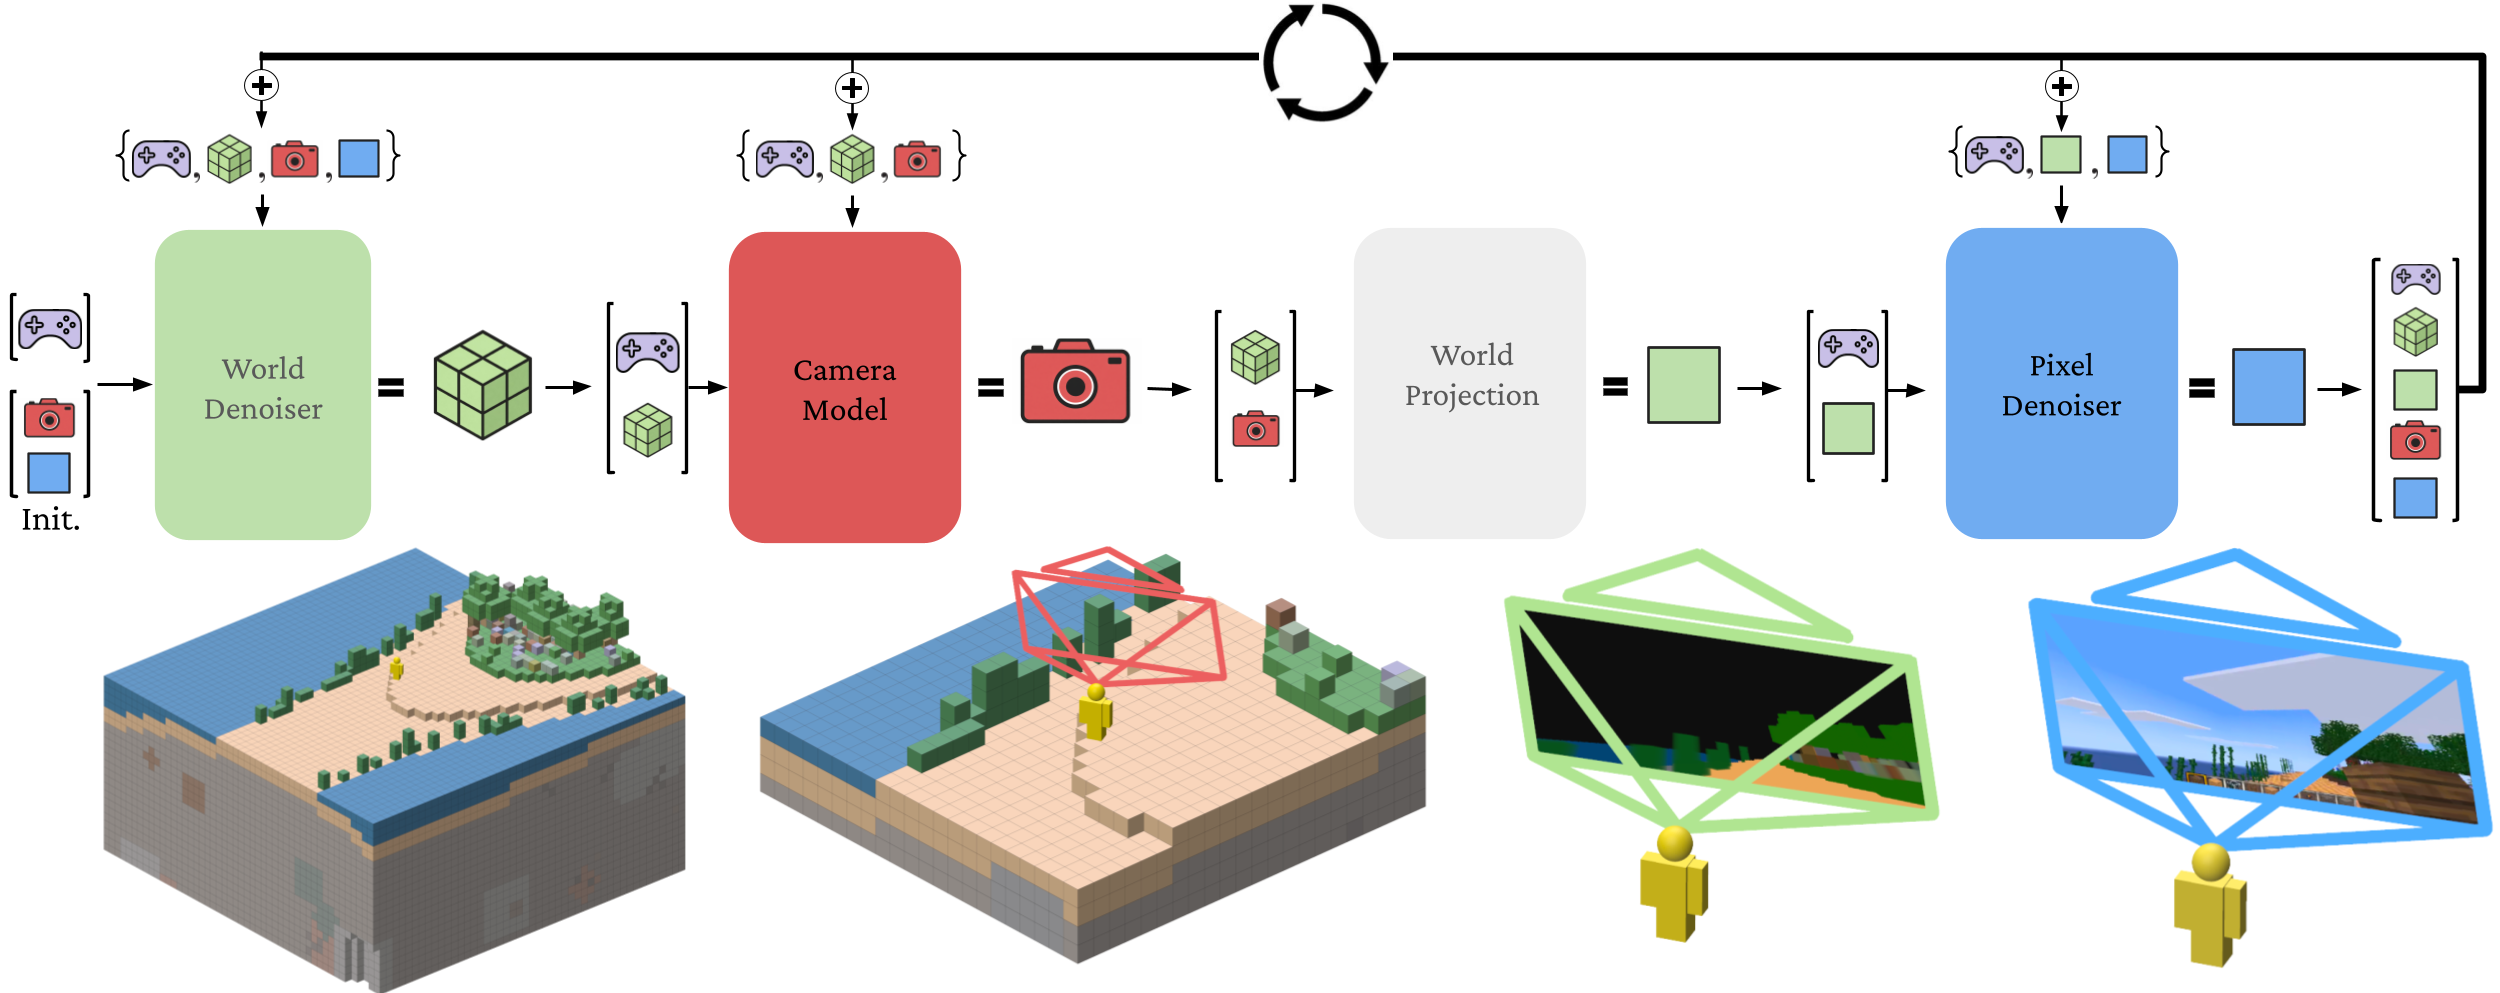
\includegraphics[width=\linewidth]{figs/Pipeline.png}}
    \caption{Initialized with a single pixel frame, PERSIST evolves in an autoregressive loop in response to user actions 
\includegraphics[height=1.5ex]{figs/action.png}. We first denoise the 3D environment centred on the agent in the form of a latent \textit{world-frame} 
\includegraphics[height=1.85ex]{figs/voxels.png}. Next, camera parameters 
\includegraphics[height=1.5ex]{figs/camera.png} are predicted with a feed-forward transformer. We then project the world to the camera plane to form a depth-ordered stack of world latents 
\includegraphics[height=1.5ex]{figs/voxel_frame.png}. Finally, pixel latents 
\includegraphics[height=1.5ex]{figs/pixel.png} are denoised, using pixel-aligned 3D information from the world latents stack 
\includegraphics[height=1.5ex]{figs/voxel_frame.png} as guidance.}
    \label{c4:fig:pipeline}
    \vspace{-0.7cm}
  \end{center}
\end{figure}



Interactive world models aim to generate experiences that unfold over time in response to user actions, enabling a new class of photo-realistic, personalised, and immersive interactive experiences for human users~\citep{kanervisto2025world, genie3, huang2025voyager}. At the same time, such models hold significant potential for safely training embodied agents within simulators learned directly from data~\citep{hafner2025training,micheli2023transformers,alonso2024diffusion,garcin2024dred}. Unlike passive video generation, interactive generation requires models to respond meaningfully to external interventions. In this setting, realism is not determined solely by per-frame visual quality, but by the degree to which the generated experience maintains persistent environments and stable dynamics throughout extended rollouts.

Most existing approaches to interactive video generation rely on autoregressive (AR) models that condition on the history of past observations and actions to generate the most recent frame, often using diffusion-based transformers with causal attention~\cite{peebles2023scalable}.
This formulation is attractive: it naturally supports real-time action conditioning, allows generation to proceed indefinitely, and integrates cleanly with recent advances in large-scale video modelling.
As a result, AR video diffusion models form the backbone of many recent neural game engines and interactive world models~\citep{chegamegen,he2025matrix,valevski2024diffusionmodelsrealtimegame,zhang2025matrix,yu2025gamefactory}.

However, conditioning on high-dimensional visual observations is computationally expensive, and the number of prior frames that AR models can ingest is tightly constrained by hardware.
In practice, this limits AR generation to condition on what amounts to only a few seconds of past footage, even when observations are compressed to lower spatial and/or temporal resolutions using learned autoencoders.
As a result, a growing body of work has explored how best to populate this limited contextual window, most commonly through heuristic strategies that retrieve individual key frames from a memory bank of past observations~\citep{xiao2025worldmem,huang2025memory}.

Yet, an inherent flaw of key-frame retrieval methods is that each pixel observation provides only partial, redundant, and viewpoint-dependent information about the world at a fixed point in time.
As the memory bank grows, identifying the relevant past evidence becomes increasingly difficult.
As a result, generating extended and coherent experiences within complex 3D environments remains an open challenge.% even for frontier models.\footnote{Closed-source frontier models report achieving up to one minute of visual memory, representing the current frontier of AR generation~\citep{genie3}.}

In this work, we propose to depart from pixel-based histories and substitute key frame retrieval with \textit{active key frame generation}.
We are inspired by traditional 3D simulators and game engines, which maintain coherence by directly rendering pixel frames from a persistent and dynamically evolving 3D state of the world. We introduce PERSIST, a framework that brings persistence to learned AR world models by tracking a dynamic 3D representation of the environment. We describe our framework in \Cref{c4:fig:pipeline}.
PERSIST decomposes world simulation into three coupled components: a \textit{world-frame model} that predicts how a learned representation of a 3D scene evolves over time, a \textit{camera model} that tracks the agent’s viewpoint within this scene, and a \textit{world-to-pixel generation module} that produces observations via differentiable projection and a learned rendering function.

Rather than treating pixels as the primary carrier of memory, PERSIST models the structure and dynamics of the environment in a latent 3D space.
This persistent world representation captures how the scene evolves over time, while the camera acts as a query mechanism that extracts the subset of 3D information relevant to guide the generation of the current frame.
This formulation enables long-horizon rollouts with fixed-cost memory, enforces geometric consistency by construction, and remains fully learned and compatible with modern diffusion and flow-based training objectives.

We evaluate PERSIST in a complex 3D environment and find that explicitly modelling persistent 3D dynamics leads to substantially improved long-horizon generation quality compared to rolling-window and memory-retrieval baselines.
Our approach exhibits stronger temporal stability, improved spatial memory when revisiting previously observed regions, and markedly better 3D consistency overall.
Beyond quantitative gains, persistent world representation enables new capabilities, including explicit 3D scene initialisation, mid-episode scene edits, 
and the emergence of off-screen dynamic processes that continue to evolve even when not directly observed.

\section{Related Work}


\begin{figure}[ht]
  \begin{center}
    \centerline{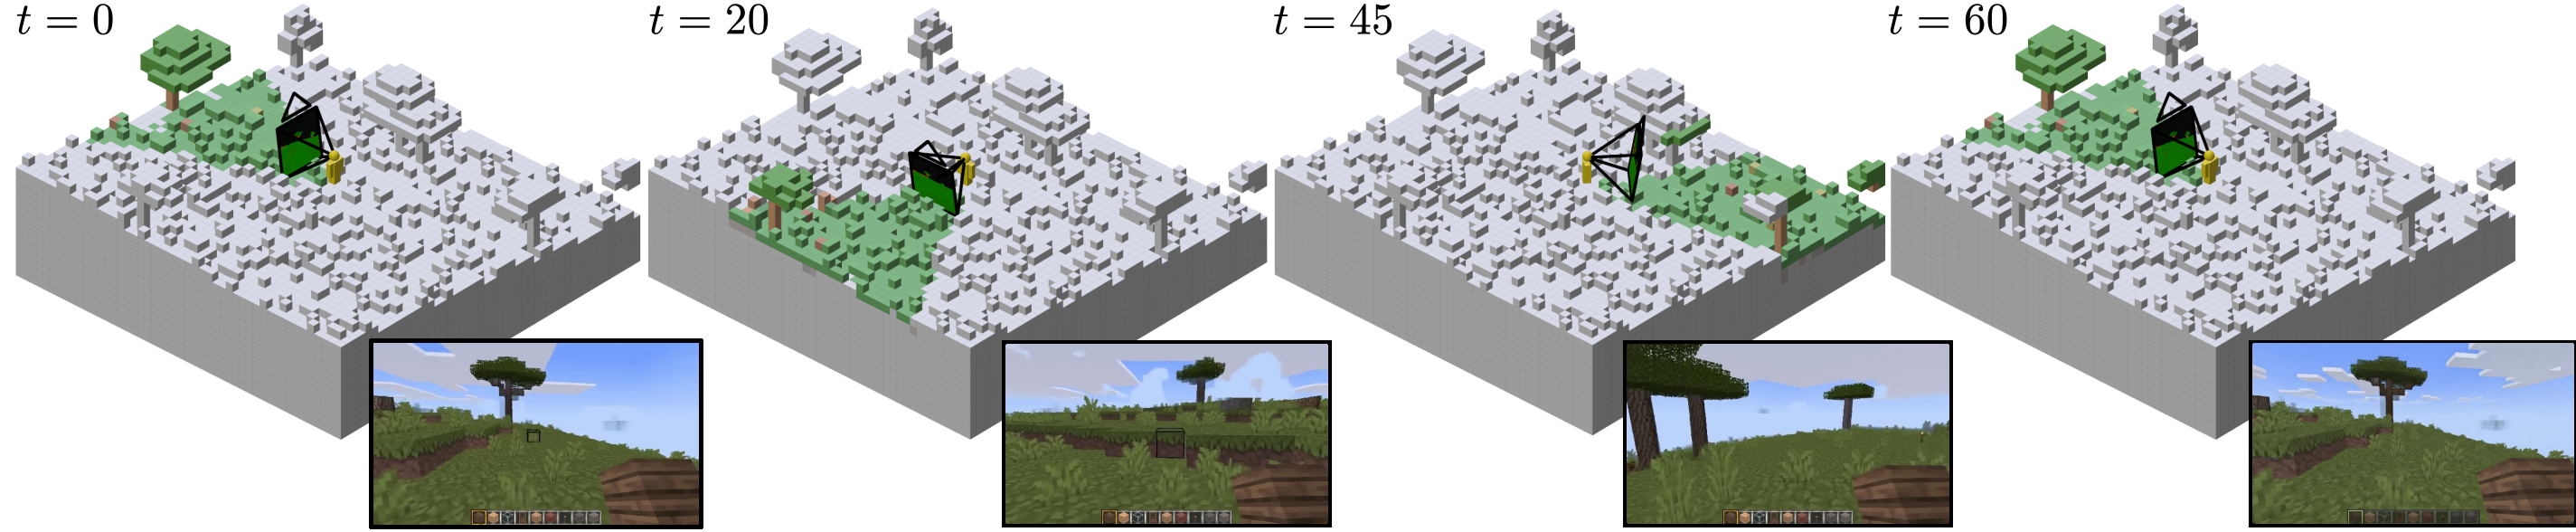
\includegraphics[width=0.95\linewidth]{figs/rotate_rgb.png}}
    \caption{PERSIST enables long-horizon spatial memory by modelling the dynamics of a 3D world-frame 
\includegraphics[height=2ex]{figs/voxels.png} around the agent. Camera parameters 
\includegraphics[height=1.5ex]{figs/camera.png} then act as memory look-up key, fetching relevant features from the world frame via a geometric projection (here visualized as the coloured voxels).} 
    \label{c4:fig:rollout-rotate}
    \vspace{-0.8cm}
  \end{center}
\end{figure}

%\textbf{Rectified flow models.}
%Rectified flow treats generation as learning a velocity field that transports noise to data with low-variance supervision and efficient sampling~\citep{lipman2022flow}. This objective has been shown to be compatible with transformer backbones and latent-space training, and integrates with DiT-style architectures~\citep{peebles2023scalable}. Leveraging this compatibility, we parameterise both world-frame and pixel-space denoisers as conditional rectified flow models, thereby enabling action-conditioned denoising given a fixed context. This formulation supports efficient per-step updates that preserve training stability while reducing inference cost, while also keeping a single objective across modules and horizons.

% \textbf{Video denoising models.}
% Recent advances in denoising models have led to substantial progress in video generation, extending image synthesis techniques to produce temporally coherent videos.
% Recent methods adopt transformer-based designs~\citep{peebles2023scalable}, but are limited to generating short video clips, due to the poor scaling of attention with video length. Auto-regressive video generation denoises frames sequentially, and has emerged as a promising direction for extending video sequences indefinitely~\citep{huang2025self}.

%mention key-frame retrieval in this sentence?
\textbf{World models.} World models~\citep{haworldmodels2018} aim to simulate environments by predicting future states conditioned on user actions. Recent progress in video generation models enables high-fidelity interactive simulation~\citep{genie3,alonso2024diffusion,decart2024oasis}. However, maintaining spatial and temporal consistency over extended rollouts remains challenging due to the finite number of past frames existing models can incorporate as context. Prior works propose to alleviate this limitation via spatio-temporal compression of input tokens ~\citep{hafner2025training}, memory-efficient attention mechanisms~\citep{po2025long} or by populating the model context window with frames sampled from the full generation history~\citep{song2025history}. Among this latter class of approaches, \cite{xiao2025worldmem,huang2025memory} propose sampling strategies that retrieve key-frames according to their spatial relevance. Nevertheless, such methods rely on retrieving relevant information from an ever-growing history of pixel observations, a task that becomes increasingly difficult and costly over extended rollouts. In contrast, PERSIST retrieves contextual information directly from a dynamically evolving 3D latent state, making its information retrieval mechanism independent of episode length.

\textbf{3D environment representations.} In parallel, a growing number of approaches incorporate explicit 3D representations into their generative architectures to produce explorable and spatially consistent environments~\citep{huang2025voyager,marble,zhou2025learning}. However, these environments remain static, restricting interaction to basic navigation within a frozen world. In contrast, PERSIST learns a 3D representation that evolves over time, enabling it to capture dynamic processes occurring within the environment, and richer agent–environment interactions.

\textbf{Neural rendering.} While neural radiance fields (NeRFs) have become a popular, compact, and resolution-free representation of 3D scenes~\citep{mildenhall2021nerf, muller2022instant, li2023neuralangelo}, they rely on costly ray marching with many neural network queries, making them prohibitively expensive for interactive use. PERSIST instead takes inspiration from neural deferred shading, which rasterizes explicit geometry into screen-space features and decodes them with learned neural shaders, enabling more efficient rendering~\citep{thies2019deferred, worchel2022multi, walker2023explicit, chen2023mobilenerf, deering1988triangle}.
% \textbf{Neural rendering.} In recent years, neural radiance fields have seen increasing usage in computer graphics as a compact and resolution-free parametrisation of 3D scenes~\citep{mildenhall2021nerf, muller2022instant, li2023neuralangelo}.
% Popularized by NeRF~\citep{mildenhall2021nerf}, these techniques rely on expensive ray-marching of an implicit function.
% We instead take inspiration from a real-time graphics technique known as \textit{deferred shading}~\citep{deering1988triangle}: a mesh is first rasterized into a screen-space map of geometric information, which is then decoded pixel-wise into RGB values using a screen-space shader. 
% Recently, learned neural deferred shaders~\citep{thies2019deferred, worchel2022multi, walker2023explicit, chen2023mobilenerf} have proved to be efficient alternatives to ray-marching based neural renderers.
%By leveraging highly-optimized polygon rasterization pipelines, they can achieve interactive frame rates across a wide range of compute platforms, including mobile devices~\citep{chen2023mobilenerf}.
%While these approaches have not seen much adoption due to their restriction to a fixed topology, we instead assume a fixed grid mesh of latent features, which are rasterized and processed by learned denoiser. %\todo[inline]{WIP}
\vspace{-0.25cm}
\section{Preliminaries}

\begin{figure}[ht]
  \begin{center}
    \centerline{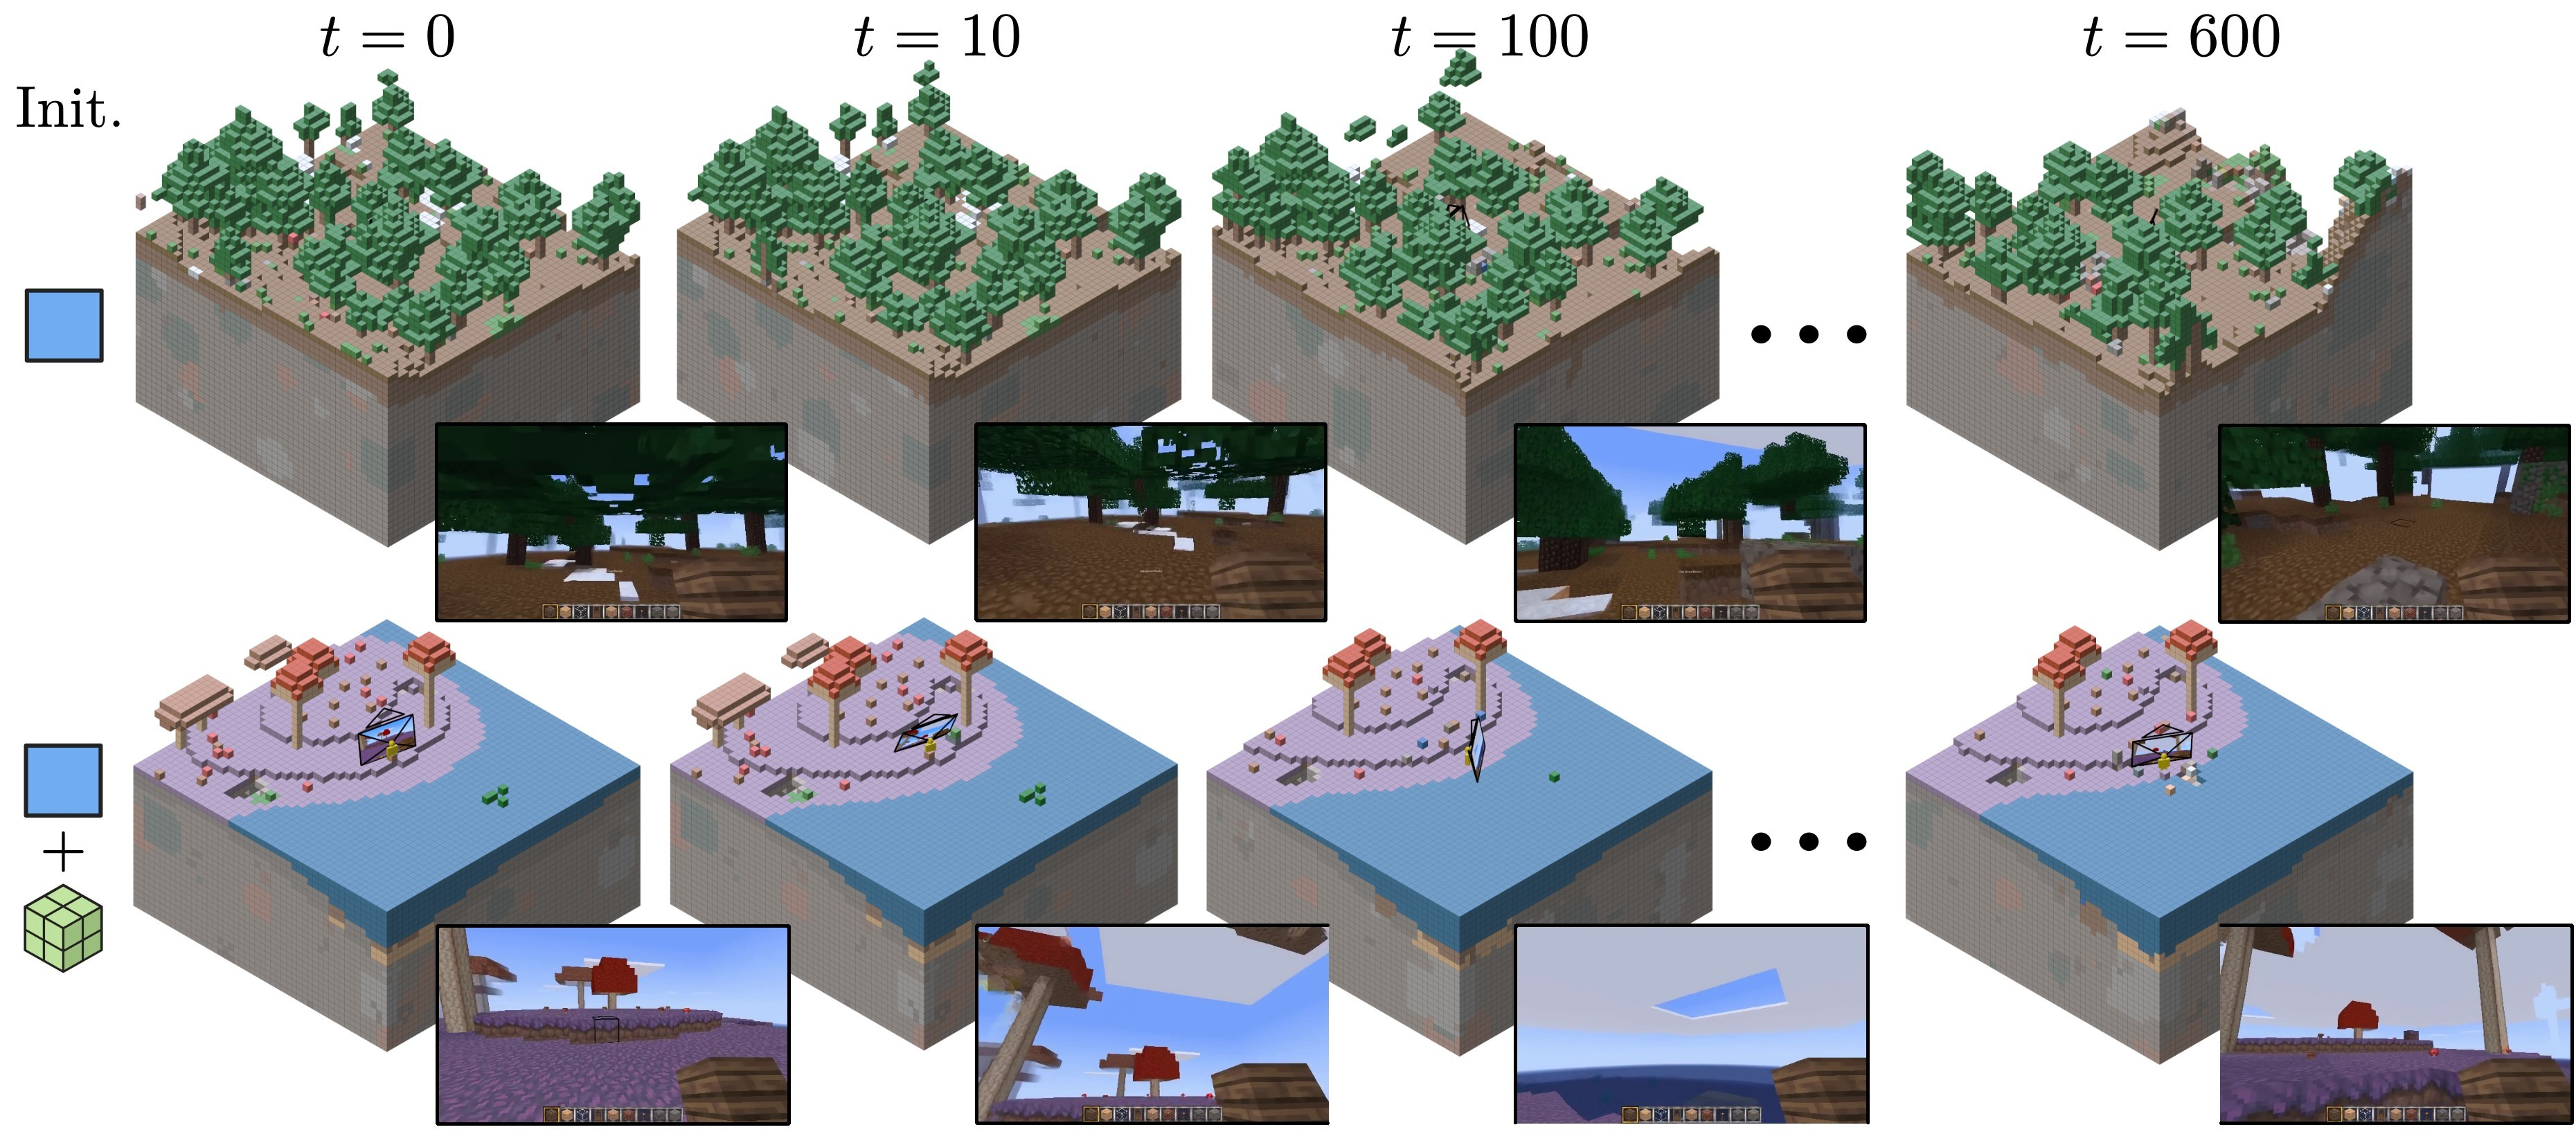
\includegraphics[width=\linewidth]{figs/qual.jpg}}
    \caption{PERSIST can be initialized with a single RGB frame (
\includegraphics[height=1.5ex]{figs/pixel.png}, row 1), or with a single RGB and world frame (
\includegraphics[height=1.5ex]{figs/pixel.png} + 
\includegraphics[height=2ex]{figs/voxels.png}, row 2). We visualize the world-frames and videos produced by an autoregressive rollout of 600 timesteps. Even with a single RGB frame for initialization, PERSIST can generate cohesive and evolving worlds.}
    \label{c4:fig:rollout-voxel}
     \vspace{-0.5cm}
  \end{center}
\end{figure}

\textbf{Rectified flow matching.} Our approach is based on the paradigm of flow matching and diffusion models~\citep{lipman2022flow}, where the task is to restore a clean data sample $x^0$ given a noised version $x^\tau$.
The noise level $\tau \in [0, 1]$ determines the degree of corruption of the data, where $\tau=0$ denotes clean data and $\tau=1$ indicates pure noise.
Rectified flow models~\citep{lipman2022flow,albergo2023building} employ a noising process $x^\tau = (1-\tau)x^0 + \tau x^1$ that linearly interpolates between sample $x^0$ and noise $x^1 \sim \mathcal{N}(0,\sI)$. 
Provided with a noised sample and corresponding noise level, the model $\gV_\theta$ is trained to predict the velocity vector $v = x^0 - x^1$ pointing towards the clean data via the conditional flow matching objective (CFM): 
\begin{equation}
    \mathcal{L}(\theta) = \norm{\gV_\theta (x^\tau, \tau) - (x^0 - x^1)}^2 \quad \tau \sim p(\tau),
\end{equation}
where $\tau$ is often sampled from a uniform or logit-normal distribution.
During inference, random noise $x^1$ is iteratively denoised into a clean sample $x^0$ over $K$ sampling steps, with uniform or variable step size $d^k$:
%
\begin{equation}
    x^{\tau - d^k} = x^\tau + \gV_\theta (x^\tau, \tau) d^k, \quad \tau \leftarrow \tau - d^k.
\end{equation}
\textbf{Autoregressive video generation.} While full-sequence video diffusion models treat videos as a single data sample to be denoised jointly at inference time, AR models treat videos as a sequence of individual frames $X^{n}_1 = x_1,x_2,\dots,x_n$ to be diffused sequentially.\footnote{Notation-wise, the noise level of an individual frame $x^\tau_t$ is indicated by superscript $\tau$, its position in the sequence by subscript $t$.
In the case of a truncated sequence $X_k^{t}$, we overload the notation to have $k$ and $t$ indicate its beginning and end.} AR models employ causal masking strategies during training to ensure no information travels from the future into the past. Diffusion forcing~\citep{chen2024diffusion}
improves the generation stability of AR video diffusion models at inference by introducing per-frame noise levels that are sampled independently during training.
At inference, AR generation becomes a special case of the training setup, where the current frame is iteratively denoised from random noise and past frames receive a small fixed noise level $\tau_\text{ctx}$.

\textbf{Interactive world simulation.} Because generation proceeds step-by-step, AR models can in principle be unrolled indefinitely and conditioned on external control signals provided at each timestep.
This enables a transition from passive video generation to interactive world simulation. We employ a similar formalism as~\citet{valevski2024diffusionmodelsrealtimegame} to characterize the problem of learning a \textit{world model}, which we define here as a learned simulator of some \textit{interactive environment} $\mathcal{E}$:
\begin{equation}
    \mathcal{E} = \langle \mathbb{S} , \mathbb{O}, \mathbb{A}, \Omega, p\rangle,
\end{equation}
 where $\mathbb{S}$ is the space of latent states, $\mathbb{O}$ the space of observations, $\mathbb{A}$ the set of actions that may be taken within the environment, $\Omega : \mathbb{S} \rightarrow \mathbb{O}$ a partial projection function mapping states to observations, and $p(s^\prime|a,s)$ is a transition probability function such that $s,s^\prime \in \mathbb{S}\times\mathbb{S}$ and $a \in \mathbb{A}$. 
Given a distribution of initial states $p_0$ and episode length $N_0$, a policy $\pi$ in charge of selecting actions in $\mathcal{E}$, and a distance metric between observation sequences $D : \mathbb{O}^n \times \mathbb{O}^n \rightarrow \mathbb{R}$, learning an interactive world simulation of $\mathcal{E}$ consists of minimising the objective $\mathbb{E}[D(O^n, \tilde{O}^n)]$. $O^n$ is a sequence of observations of length $n\sim N_0$ collected in $\mathcal{E}$ from starting state $s_0\sim p_0$ and by following $\pi$; and $\tilde{O}^n$ is obtained from an AR model $\gQ_\theta$ initialised at $\vo_0 = \Omega(s_0)$ and subjected to the same action sequence.

\vspace{-0.2cm}
\section{A Persistent Environment Representation}
Learning an autoregressive model $\gQ_\theta$ is often challenging when $\mathcal{E}$ is a complex 3D environment featuring high dimensional pixel observations.
First, memory constraints limit $\gQ_\theta$ to condition on a finite context window of past $K$ frames, which degrades temporal consistency once the generated episode exceeds this horizon. 
Second, pixel observations typically provide partial information about the environment's hidden state, making learning accurate transition dynamics challenging.
One might therefore attempt to have $\gQ_\theta$ condition on some approximation of the hidden state $s$; however $s$ can be arbitrarily complex or entirely unmeasurable. Even if $s$ were accessible, learning the observation function $\Omega : \sS \rightarrow \sO $ to recover observations can be a comparably challenging problem. For example, in the case of a video game, $s$ would be the program's dynamic memory contents, which may not be particularly helpful for easily recovering pixel observations. 

Instead, we define a proxy $\tilde{s} = \langle \vw, \vc \rangle$, where $\vw$ is a \textit{world-frame} representing a fixed region of space centred on the agent, and $\vc$ is a camera state encoding the agent's view within $\vw$.
Although not a perfect replacement for the true hidden state, $\tilde{s}$ is an effective modelling choice when $\mathcal{E}$ is a 3D environment, as it lets us:
%todo reduce spacing [noitemsep]
\begin{enumerate}[leftmargin=*,nosep]
    \item \textbf{Simplify information retrieval.} \Cref{c4:fig:rollout-rotate} demonstrates how the world-frame $\vw_t$ can function as a dynamic \textit{spatial memory} module throughout the episode, while the camera state $\vc_t$ acts as a \textit{spatial lookup key} to retrieve the spatial information in $\vw_t$ that is necessary to reconstruct $\vo_t$. $\vc_t$ encodes the information to project this information to screen-space, without requiring explicit knowledge of the true observation function.
    \item \textbf{Improve dynamics predictions.} Tracking $\vw$ and $\vc$ over time facilitates modelling dynamics that are difficult to infer from pixel observations alone, such as interactions or collisions with out-of-view objects, or tracking how occluded regions of the environment change over time.
\end{enumerate}



\vspace{-0.26cm}
\section{PERSIST}
We present PERSIST (Persistent Environment Representations for Simulating Interactive Space-Time), a world simulation framework for complex 3D environments.
PERSIST decomposes the world simulation objective into the tasks of \textit{world frame prediction}, \textit{camera prediction} and \textit{world-to-pixel generation}.

\textbf{Dataset construction and pre-processing.} The different components of PERSIST are trained from a dataset of trajectories collected from $\mathcal{E}$.
A trajectory consists of a sequence of pixel observations $O$, actions $A$, world-frames $W$ and camera views $C$.
In this work, we assume that $W$ and $C$ are directly obtainable from $\mathcal{E}$, the former as a 3D voxel grid within a cuboid centred on the agent, and the latter as a vector encoding the camera intrinsics and extrinsics.
Actions are embedded as a 23-dimensional multi-hot encoding of key presses and discretised mouse movements.
We train a 2D-VAE and a 3D-VAE to encode pixel- and world-frames into latent patches $\bar{\vo}$ and $\bar{\vw}$ of 10$\times$10 pixels and $4^3$ voxels respectively. 

\subsection{World-Frame and Camera Prediction}

\textbf{World frame prediction.} At each timestep, a new world-frame is generated by sampling 
\begin{equation}
  \bar{\vw}_t \sim \gW_\theta(\bar{\rvw_t} | \bar{W}^{t-1}_{t-K}, A^t_{t-K}, C^{t-1}_{t-K-1}, \bar{O}^{t-1}_{t-K-1}),  
\end{equation}
where $K$ is the model's temporal context window and latents $\bar{W}^{t-1}_{t-K}$ and $\bar{O}^{t-1}_{t-K-1}$ are encoded using the VAEs. 
$\gW_\theta$ is parametrised as a rectified flow model with a causal Diffusion Transformer (DiT) backbone~\citep{peebles2023scalable} employing interleaved spatial, temporal and cross-attention modules~\citep{decart2024oasis}.
We modify the spatial module to handle three spatial dimensions, and replace RoPE spatial embeddings~\citep{su2024roformer} with absolute position embeddings of the XYZ coordinates of the centroid of each voxel token.
We keep the temporal module as-is.
Actions and cameras are jointly embedded using a multi-layer perceptron (MLP).
The resulting embeddings are added to the denoising timestep embedding and injected into each module via Adaptive Layer Normalisation (AdaLN)~\citep{peebles2023scalable}. We concatenate pixel patches channel-wise with Pl\"ucker embeddings~\citep{xiao2025worldmem,sitzmann2021light} computed from $C^{t-1}_{t-K-1}$ to convey 3D projection information. The resulting patches are then injected into the model via the cross-attention module.
Finally, we employ the 3D-VAE to decode $\bar{\vw}_t$ to its native resolution.

Crucially, $\gW_\theta$ supports conditioning on $\bar{W}=\varnothing$, making it capable of generating the initial world frame $\vw_0$ from initial condition $\langle \vo_0, \vc_0 \rangle$ at inference time.
Thus, while we rely on $W$ to train $\gW_\theta$, we do not have to rely on ground truth 3D conditioning during inference. We provide examples for each inference configuration in \Cref{c4:fig:rollout-voxel}.


% \textbf{Dynamic loss.}

\textbf{Camera model.} At any given timestep, the cameras is represented as the 10-dimensional vector $\vc = \langle\textbf{pos}, \textbf{rot}, \text{fov}\rangle$, where $\textbf{pos}\in \sR^3$ encodes the camera's position in the world-frame, $\textbf{rot}\in \sR^6$ its orientation as a 6D continuous rotation~\citep{zhou2019continuity}, and $\text{fov}\in \sR$ its field-of-view. The camera model predicts $\vc_{t} = \gC_\theta (C^{t-1}_{t-1-K}, W^t_{t-K}, A^t_{t-K})$ using a 1D causal transformer backbone with RoPE temporal embeddings. Individual tokens are obtained by passing $\textbf{pos}$ and $\textbf{rot}$  through separate positional embedders, concatenating $\text{fov}$ and applying a linear projection. $W$ is cropped to its inner-most $4^3$ voxels and embedded alongside $A$ via a joint MLP prior to AdaLN injection. Given that the camera only rotates along its pitch and yaw axis, we re-parametrise the model's output layer to predict $\bar{\vc}=\langle \textbf{pos}, \Delta\text{pitch}, \Delta\text{yaw}, \Delta\text{fov}\rangle$, with residuals $\Delta\text{pitch} = \text{pitch}_t - \text{pitch}_{t-1}$,$\Delta\text{yaw} =\text{yaw}_t - \text{yaw}_{t-1}$ and $\Delta \text{fov}=\text{fov}_t - \text{fov}_{t-1}$.\footnote{$\vc_t$ is recovered from $\langle \bar{\vc}_t, \vc_{t-1}\rangle$ via an algebraic manipulation at inference time.} The camera model is trained via MSE losses applied to each component of $\bar{\vc}$.

\subsection{World-to-Pixel Generation}

In order to condition the pixel-space generation on 3D information we need to form world-to-pixel correspondence.

\textbf{World projection.} We project $\vw$ to screen-space via the projection operator \begin{equation}
    \mathcal{R}(\vc, \vw) = (\tilde{\vw}_{2D}, \vd), 
\end{equation}
where $\tilde{\vw}_{2D}  \in \mathbb{R}^{h \times w \times l \times m}$ is a per-pixel depth-ordered list of $l$ voxel features with $m$ channels, indexed according to their position in screen space $\langle h_i, w_j\rangle$. $\vd \in \mathbb{R}^{h \times w \times l}$ is the linear depth of each voxel feature measured in camera space. We provide a visualisation of how $\mathcal{R}$ constructs $\tilde{\vw}_{2D}$ and $\vd$ in \Cref{c4:fig:render}. $\mathcal{R}$ employs the same $h,w$ screen dimensions as the pixel latents, ensuring pixel-level alignment with $\bar{\vo}$. Finally, we combine $\tilde{\vw}_{2D}$ and $\vd$ into $\vw_{2D}\in \mathbb{R}^{h \times w \times z}$ via channel-wise concatenation, where $z = l \times (m+1)$. %We use the CUDA-accelerated differentiable rasterization provided by~\citep{Laine2020diffrast} to generate $(\vw_{2D}, \vd)$ via a fixed-cost, single feedforward operation.


% Since we model a camera $\vc$ and 3D world-frame $\vw$, we can provide $\mathcal{P}_\theta$ with pixel-level conditioning on the relevant 3D features $\vw$ via a differentiable projection $\mathcal{R}(\vc, \vw)$ to screen-space. We then leave the final rendering step as a learned process for the screen-spa3ce denoiser $\mathcal{P}_\theta$. This choice allows the pixel denoiser to learn arbitrary compositing functions, whilst still enforcing geometric consistency through analytic projections of the 3D world.
% We define the projection operator $\mathcal{R}$ as 
% \begin{equation}
%     \mathcal{R}(\vc, \vw) = (\vw_{2D}, \vd), 
% \end{equation}
% where $\vw_{2D}  \in \mathbb{R}^{h \times w \times l \times m}$ represents a per-pixel depth-ordered list of $l$ voxel features with $m$ channels, indexed according to their position in screen space $\langle h_i, w_j\rangle$. $\vd \in \mathbb{R}^{h \times w \times l}$ represents the linear depth of each voxel feature measured in camera space. To ensure pixel-level alignment between 2D and 3D latents, we rasterize $\vw$ using the same $h,w$ screen dimensions as the pixel latents. For projection, we use the CUDA-accelerated differentiable rasterization 
% provided by~\citep{Laine2020diffrast}. For details, please see the appendix.

\begin{figure}[ht]
    \centering
    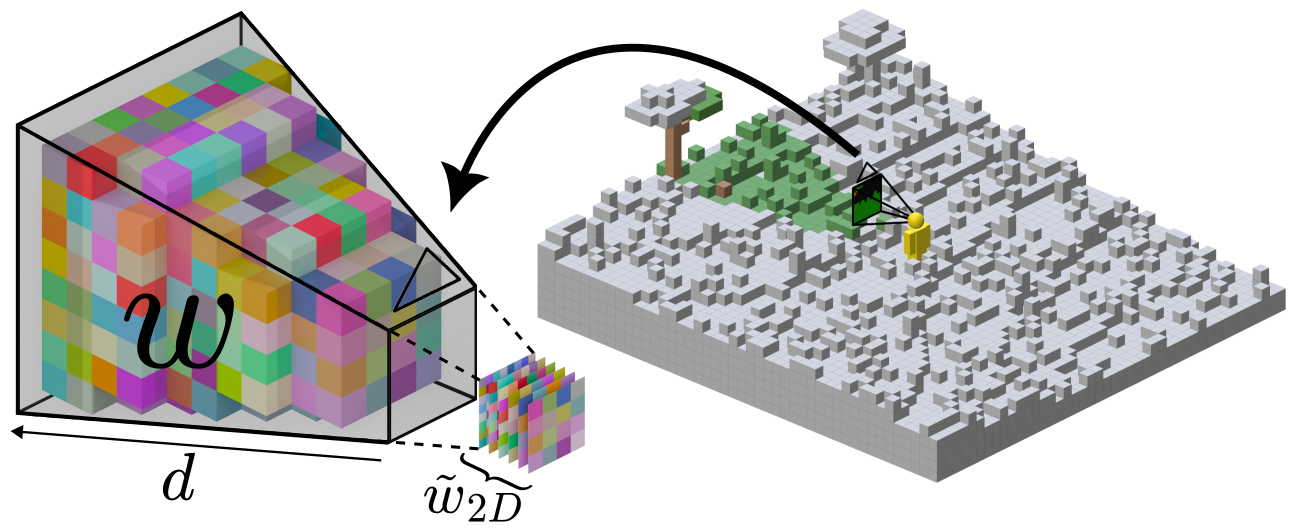
\includegraphics[width=0.9\linewidth]{figs/renderer.png}
    \vspace{-0.1cm}
    \caption{World frame $\vw$ features are projected to screen-space to obtain the depth-ordered stack of features $\tilde{\vw}_{2D}$ and linear depth information $\vd$.}
        \vspace{-0.2cm}
    \label{c4:fig:render}
\end{figure}



 

% While surrounding works~\cite{xiao2025worldmem,huang2025memory} employ camera tracking to retrieve a key frame from a memory bank of past pixel observations, $\mathcal{R}$ lets PERSIST \textit{generate} a new key frame from the current world-frame representation $\vw_t$ via a fixed-cost, single feedforward operation.

\textbf{Pixel frame prediction.}
Pixel frames are generated by sampling
\begin{equation}
    \bar{\vo}_t \sim \gP_\theta (\bar{\rvo}_t | {W_{2D}}_{t-K}^{t}, A^t_{t-K}, \bar{O}^{t-1}_{t-K}),
\end{equation}
where ${W_{2D}}_{t-K}^{t}$ is obtained from the projection $\gR(C_{t-K}^{t},W_{t-K}^{t})$. Here, $\gP_\theta$ acts as a learned deferred shader~\cite{thies2019deferred} which additionally predicts information not provided by 3D latents (e.g. texture, lighting, particle effects, screen-space overlays, \ldots). This choice allows $\gP_\theta$ to learn arbitrary rendering functions, whilst encouraging spatial consistency through its dependency on $\vw_{2D}$. $\gP_\theta$ is parametrised as a rectified flow model with a causal DiT backbone employing interleaved spatial and temporal modules~\citep{decart2024oasis}. Actions are embedded using a MLP and injected via AdaLN. $\vw_{2D}$ is projected to latent space via a channel-wise 1D-convolution and is incorporated to $\bar{\vo}$ via channel-wise concatenation. Crucially, we assign more latent channels to $\vw_{2D}$ than to $\bar{\vo}$, in order to bias the model to use the 3D latent frame as its primary source of information.

\vspace{-0.24cm}
\subsection{Mitigating Exposure Bias}

During training, the denoisers condition on latents encoded from the training data. However, they condition on autoregressive predictions at inference time, leading to exposure bias~\citep{ning2023elucidating}. We train each denoiser with diffusion forcing~\citep{chen2024diffusion} to make them robust to the exposure bias induced by their own predictions. In addition, at inference $\gW_\theta$ depends on latents predicted by $\gP_\theta$, and vice-versa. To alleviate the resulting distributional shift, we apply a flat 10\% random noise augmentation to $\bar{O}$ when training $\gW_\theta$, and to $\bar{W}$ when training $\gP_\theta$. This lets us train each component of PERSIST separately and combine them at inference time without any fine-tuning.

\vspace{-0.24cm}
\section{Experiments}

% More separation between methods and more levels
% Fig 2 = fig 3 + full rotation
% Fig 3 =  3 rows, pixel init, pixel + voxel init, voxel edit, 4th row dynamic?
% 

We conduct our experiments within Luanti~\citep{luanti2024}, an open-source voxel-based game engine inspired by Minecraft.\footnote{We prefer Luanti over Minecraft due to its open-source design and expressive Lua API, which facilitates data collection and experimentation.} Voxel environments discretise 3D space into individual voxels, each voxel taking on any of thousands of possible configurations (e.g. water, stone, air, etc.\ ). These environments constitute a valuable research platform~\citep{malagon2025craftium,fan2022minedojo,guss2019minerl,baker2022video}, as they instantiate interpretable, complex, diverse, and persistent 3D worlds with rich player–environment interactions. Unlike prior work that learns world models from data collected within a single game map~\citep{alonso2024diffusion,kanervisto2025world}, we learn a broad distribution of procedurally generated worlds. Training world models within procedural environments substantially increases the difficulty of achieving spatial and temporal consistency, as the model cannot overfit to a fixed environment layout.


\textbf{Dataset.} We use the Craftium platform~\citep{malagon2025craftium} to collect game data to train and evaluate our models. We collect $\sim$40M environment interactions consisting of player actions, camera states, pixel and 3D observations. Actions are represented as multi-hot vectors encoding individual key presses and discretised mouse movements. 3D observations are represented as a $48^3$ voxel grid centred on the agent. In Luanti, individual voxels contain semantic information about a specific spatial location, encoded as integer labels. In total, we collect $\sim$100K trajectories, amounting to 460 hours of gameplay recorded at 24Hz. 
To interact with the game, we employ a similar strategy as~\citep{yu2025gamefactory} and design a simple policy that randomly samples from a set of pre-defined action sequences. %\Cref{c4:app:data} provides further details on our data collection strategy.

\textbf{Training and Inference.} All models are trained using the AdamW~\citep{loshchilov2018decoupled} optimizer with a learning rate of $1e-4$. We first train the VAEs and pre-encode the 3D and pixel latents to accelerate the training of the dynamic models. The pixel and 3D VAEs take 4 and 12 days to train using 8 A100 GPUs. We train two versions of the 3D denoiser, ``3D-S'' and ``3D-XL'', which uses 8$\times$ more spatial tokens. 3D-S takes 3 days to train on 8 H100 GPUs, while 3D-XL and the pixel denoiser each take 10 days. The camera model trains on a single A100 in 16 hours with batch size 256. All other models use batch size 64. Each model is trained separately and assembled in the full pipeline with no further fine-tuning. At inference, we use 20 denoising steps per-frame and slightly noise past context frames to make the denoisers more resilient to imperfections in their own generations. We provide more implementation details in \Cref{c4:app:implt}.

\begin{figure}[ht]
  \begin{center}
    \centerline{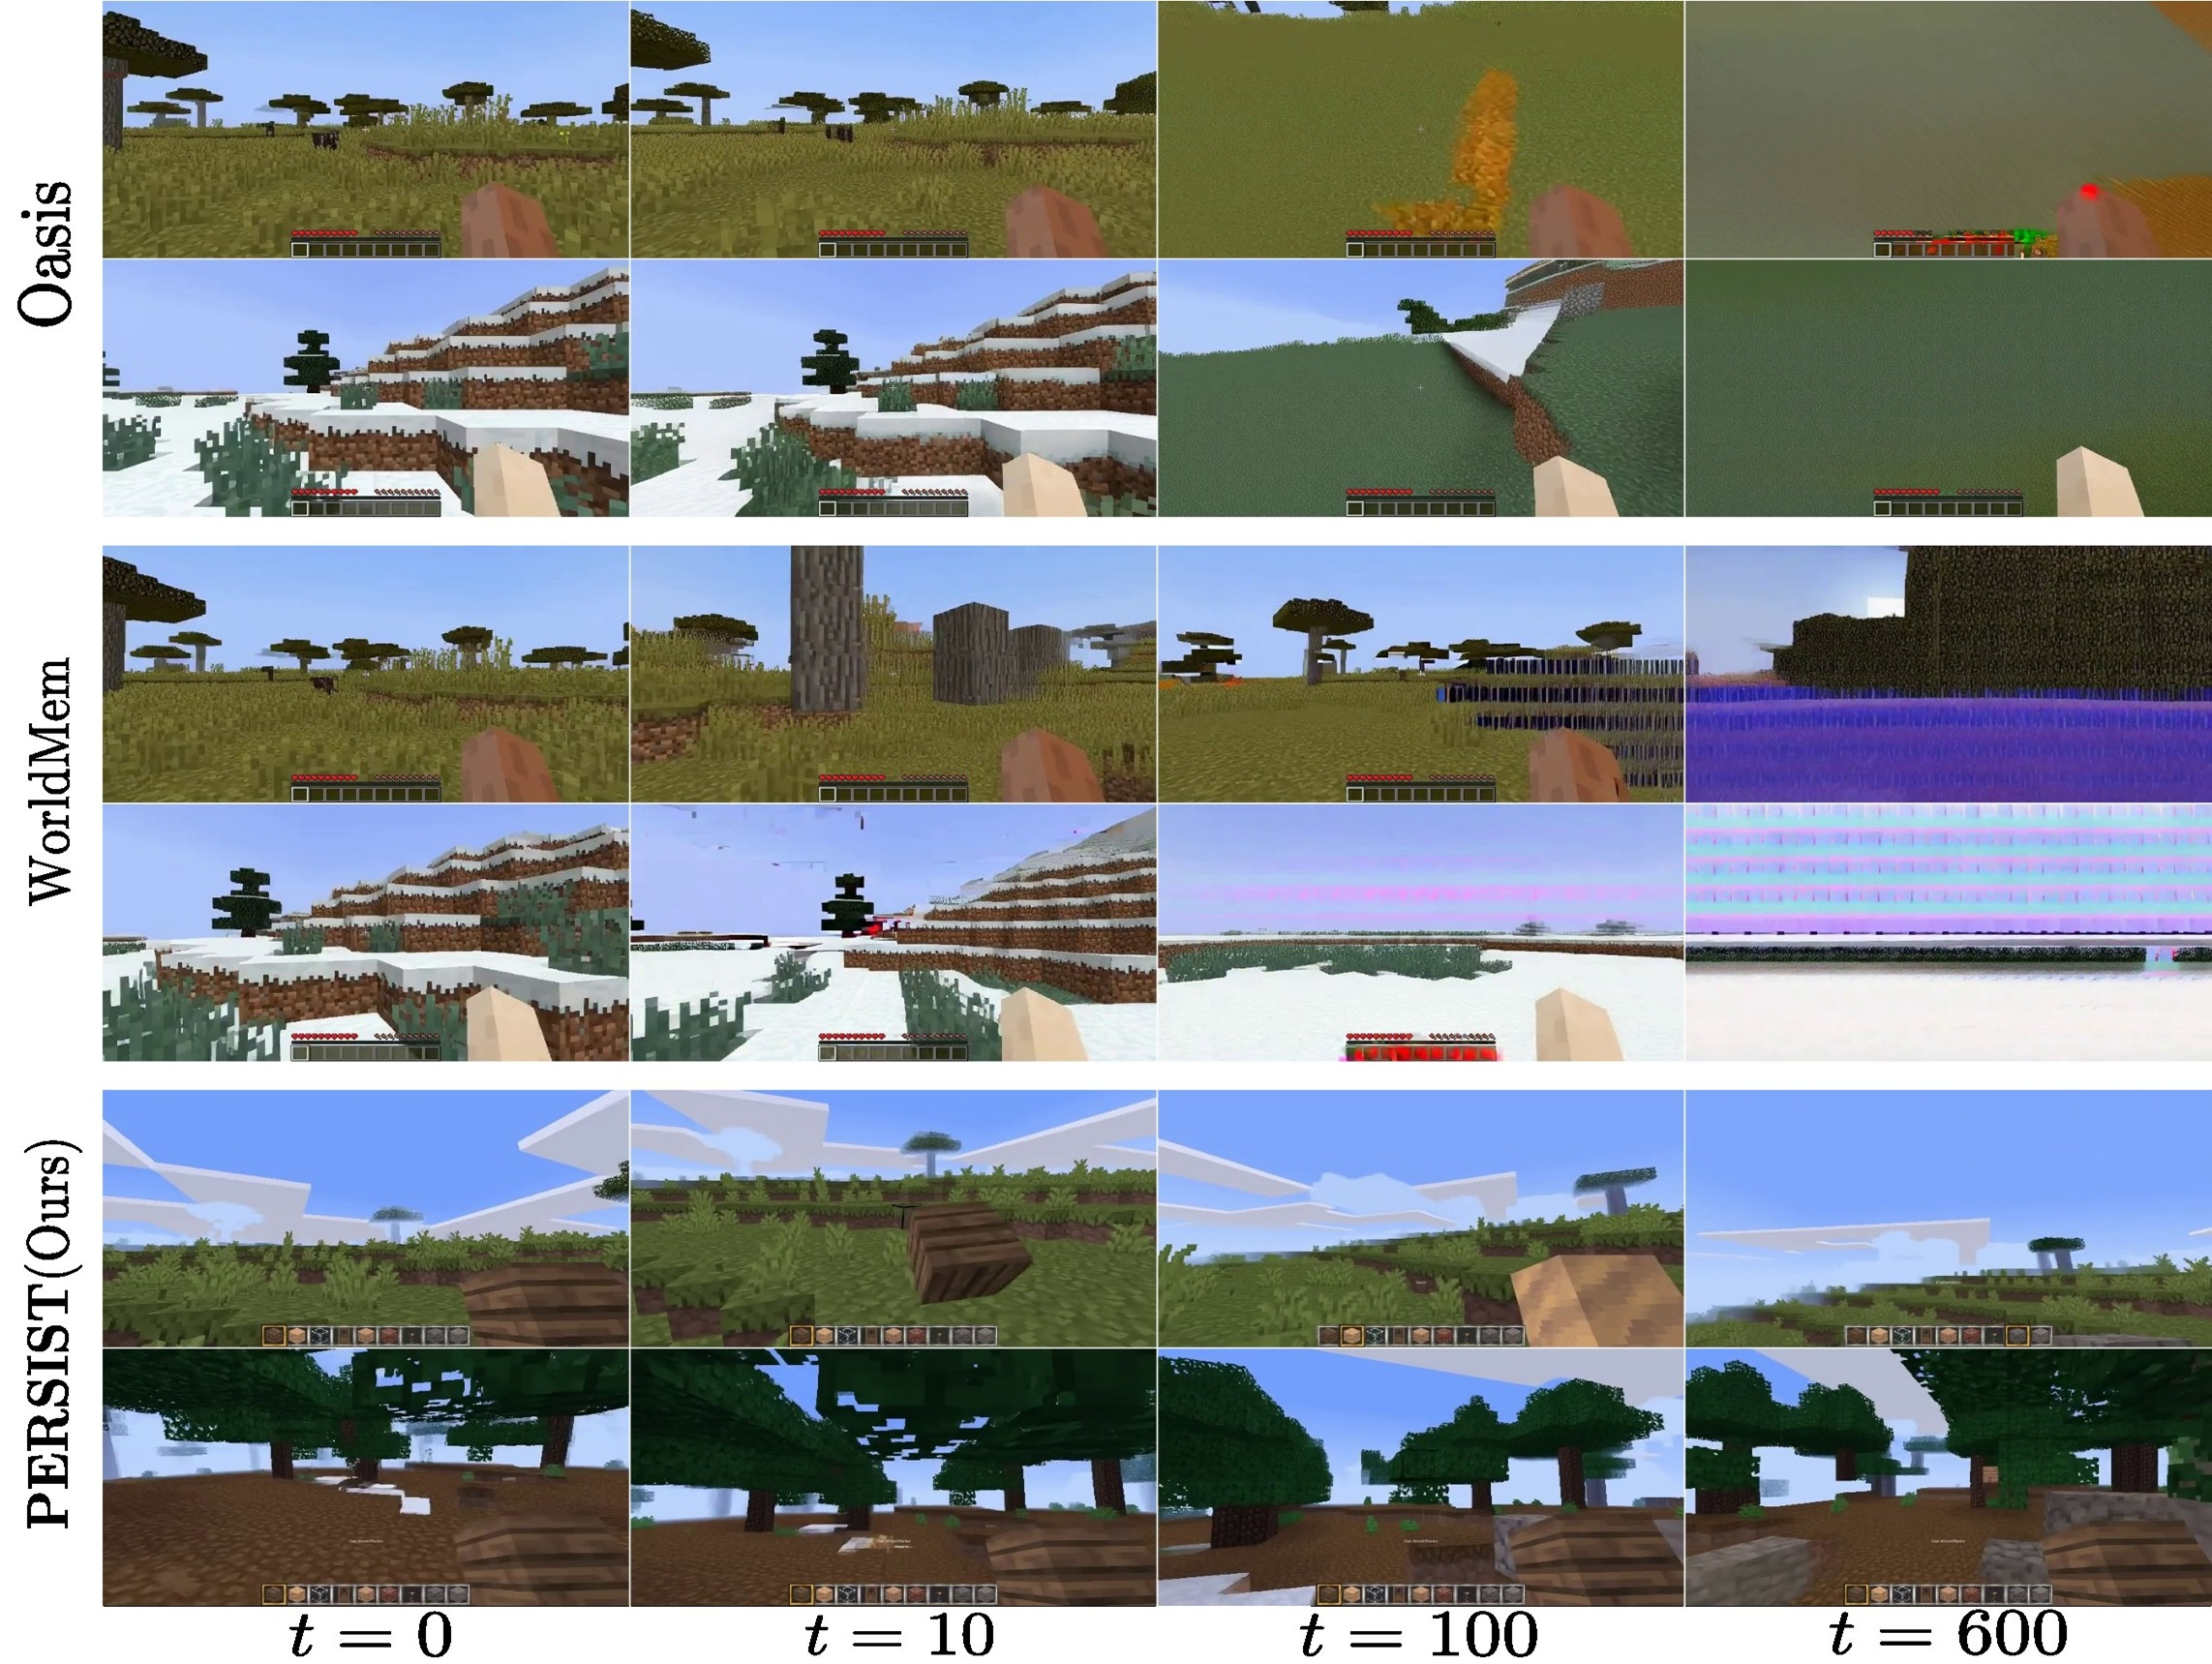
\includegraphics[width=0.87\linewidth]{figs/compare_87.jpg}}
    \caption{Video frames generated over 600 timestep episodes by PERSIST (Ours), Oasis~\citep{decart2024oasis} and WorldMem~\citep{xiao2025worldmem}.}
    \label{c4:fig:rollout}
    \vspace{-0.7cm}
  \end{center}
\end{figure}

\begin{figure}[ht]
  \begin{center}
    \centerline{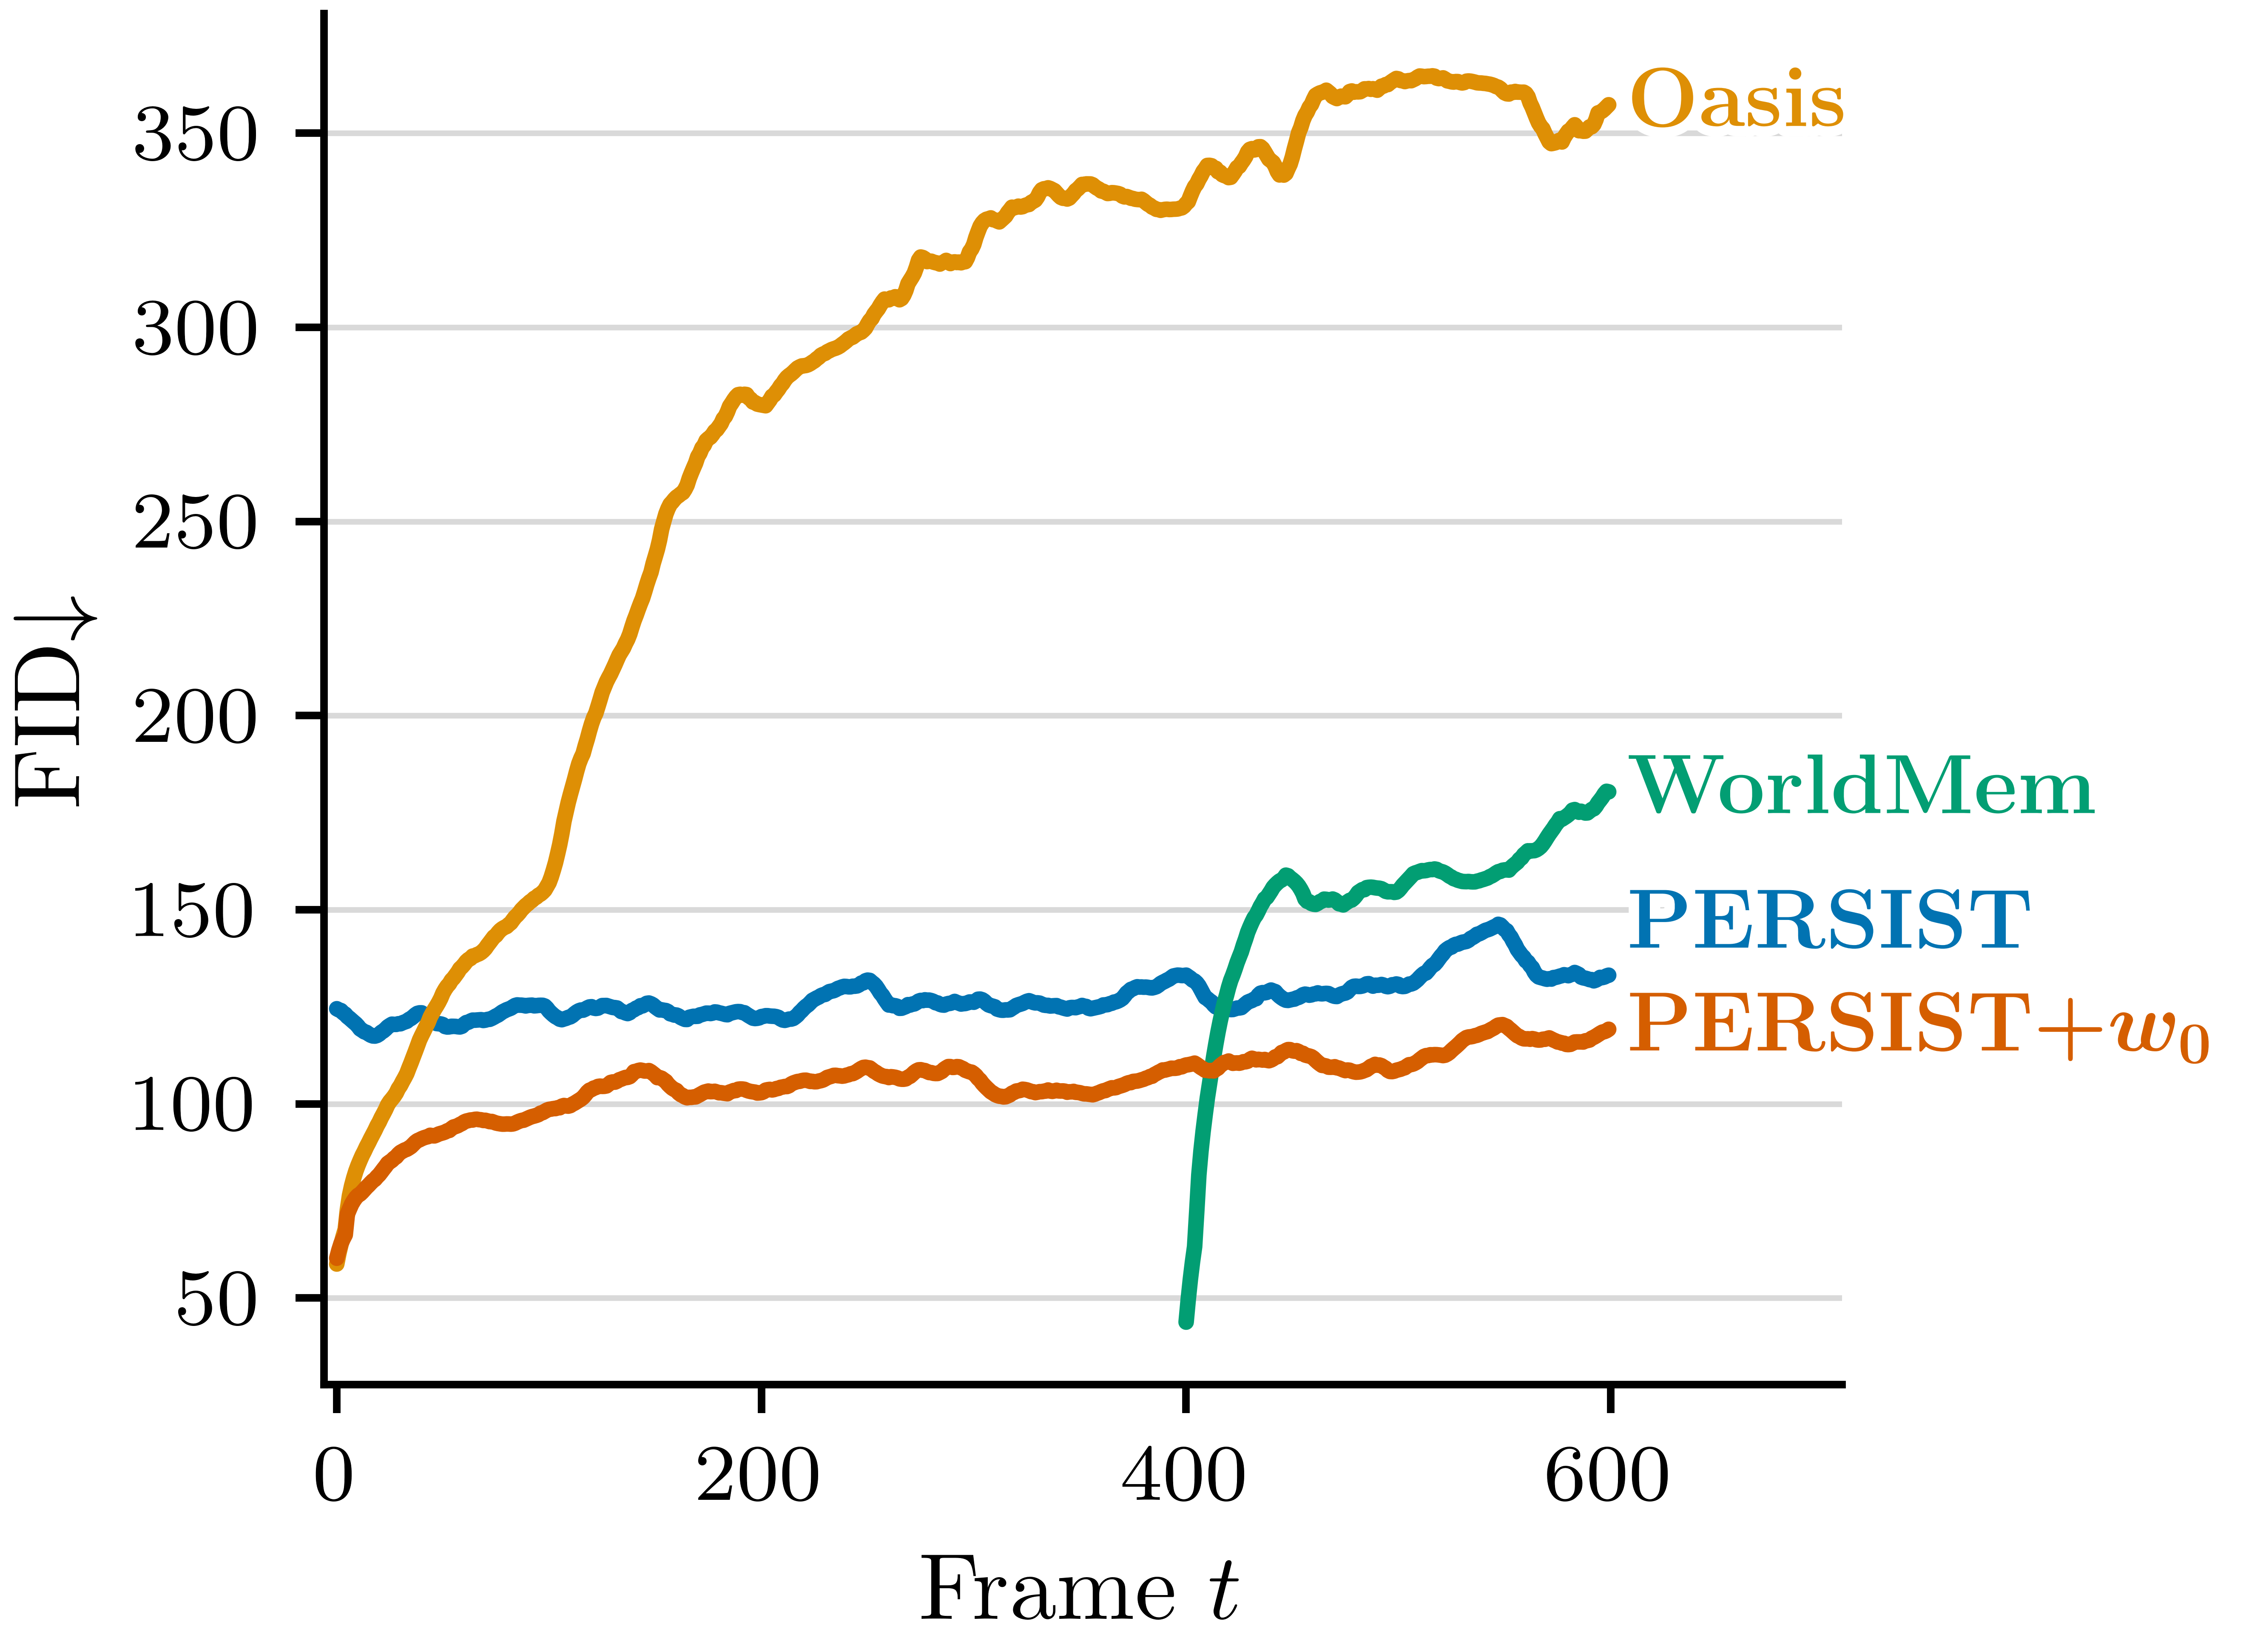
\includegraphics[width=0.69\linewidth]{figs/fid_vs_t_wmshift.png}}
    \caption{FID scores compared to ground truth over 600 frame episodes. PERSIST configurations remains stable, while baselines relying on pixel-histories degrade rapidly.}
    \label{c4:fig:fid_vs_t}
     %\vspace{-1cm}
  \end{center}
\end{figure}

\begin{table}[t]
  \centering
  \caption{FVD ($\downarrow$) evaluated across different episode lengths (200, 400, and 600 frames). We compare our base configuration (PERSIST) against pixel-history baselines and various model ablations. PERSIST$+\vw_0$ is discussed in \Cref{c4:sec:new_app}.}
  \small
  \setlength{\tabcolsep}{6pt}
  \begin{tabular}{lccc}
  \toprule
  Method & 200 Frames & 400 Frames & 600 Frames \\
  \midrule
  Oasis & 409 & 687 & 875 \\
  WorldMem & 358 & -- & -- \\
  \midrule
  No-3D-Upscale & 216 & 231 & 247 \\
  Camera-GT & 161 & 152 & 152 \\
  PERSIST-S & 159 & 170 & 179 \\
  PERSIST & \textbf{129} & \textbf{141} & \textbf{148} \\
  \midrule
  PERSIST$+\vw_0$ & 80 & 93 & 104 \\
  \bottomrule
  \end{tabular}
  \label{c4:tab:fvd}
  %\vspace{-0.095cm}
\end{table}

\begin{table}[t]
\centering
\caption{Mean user ratings (score range: 1-5) for videos generated from different PERSIST configurations and baselines. Bold numbers indicate the best performing methods. VF = Visual Fidelity, 3D = 3D Consistency, Temp = Temporal Consistency, Overall = Overall Score.}

\small
\setlength{\tabcolsep}{2.6pt}
\begin{tabular}{lcccc}
    \toprule
    Method & VF$\uparrow$ & 3D$\uparrow$ & Temp$\uparrow$ & Overall$\uparrow$ \\
    \midrule
    Oasis & 2.1 $\pm$ 0.1 & 1.9 $\pm$ 0.1 & 1.8 $\pm$ 0.1 & 1.9 $\pm$ 0.1 \\
    WorldMem & 1.7 $\pm$ 0.09 & 1.7 $\pm$ 0.09 & 1.5 $\pm$ 0.08 & 1.5 $\pm$ 0.07 \\
    PERSIST-S & \textbf{2.8 $\pm$ 0.1} & \textbf{2.7 $\pm$ 0.1} & \textbf{2.5 $\pm$ 0.1} & \textbf{2.6 $\pm$ 0.09} \\
    PERSIST & \textbf{2.8 $\pm$ 0.09} & 2.5 $\pm$ 0.09 & \textbf{2.5 $\pm$ 0.09} & \textbf{2.6 $\pm$ 0.08} \\
    \midrule
    PERSIST$+\vw_0$ & 3.2 $\pm$ 0.1 & 2.8 $\pm$ 0.1 & 2.8 $\pm$ 0.1 & 3.0 $\pm$ 0.1 \\
    \bottomrule
    \end{tabular}
    %\vspace{-0.45cm}
    \label{c4:tab:eval}
\end{table}

\begin{figure}[ht]
  \begin{center}
    \centerline{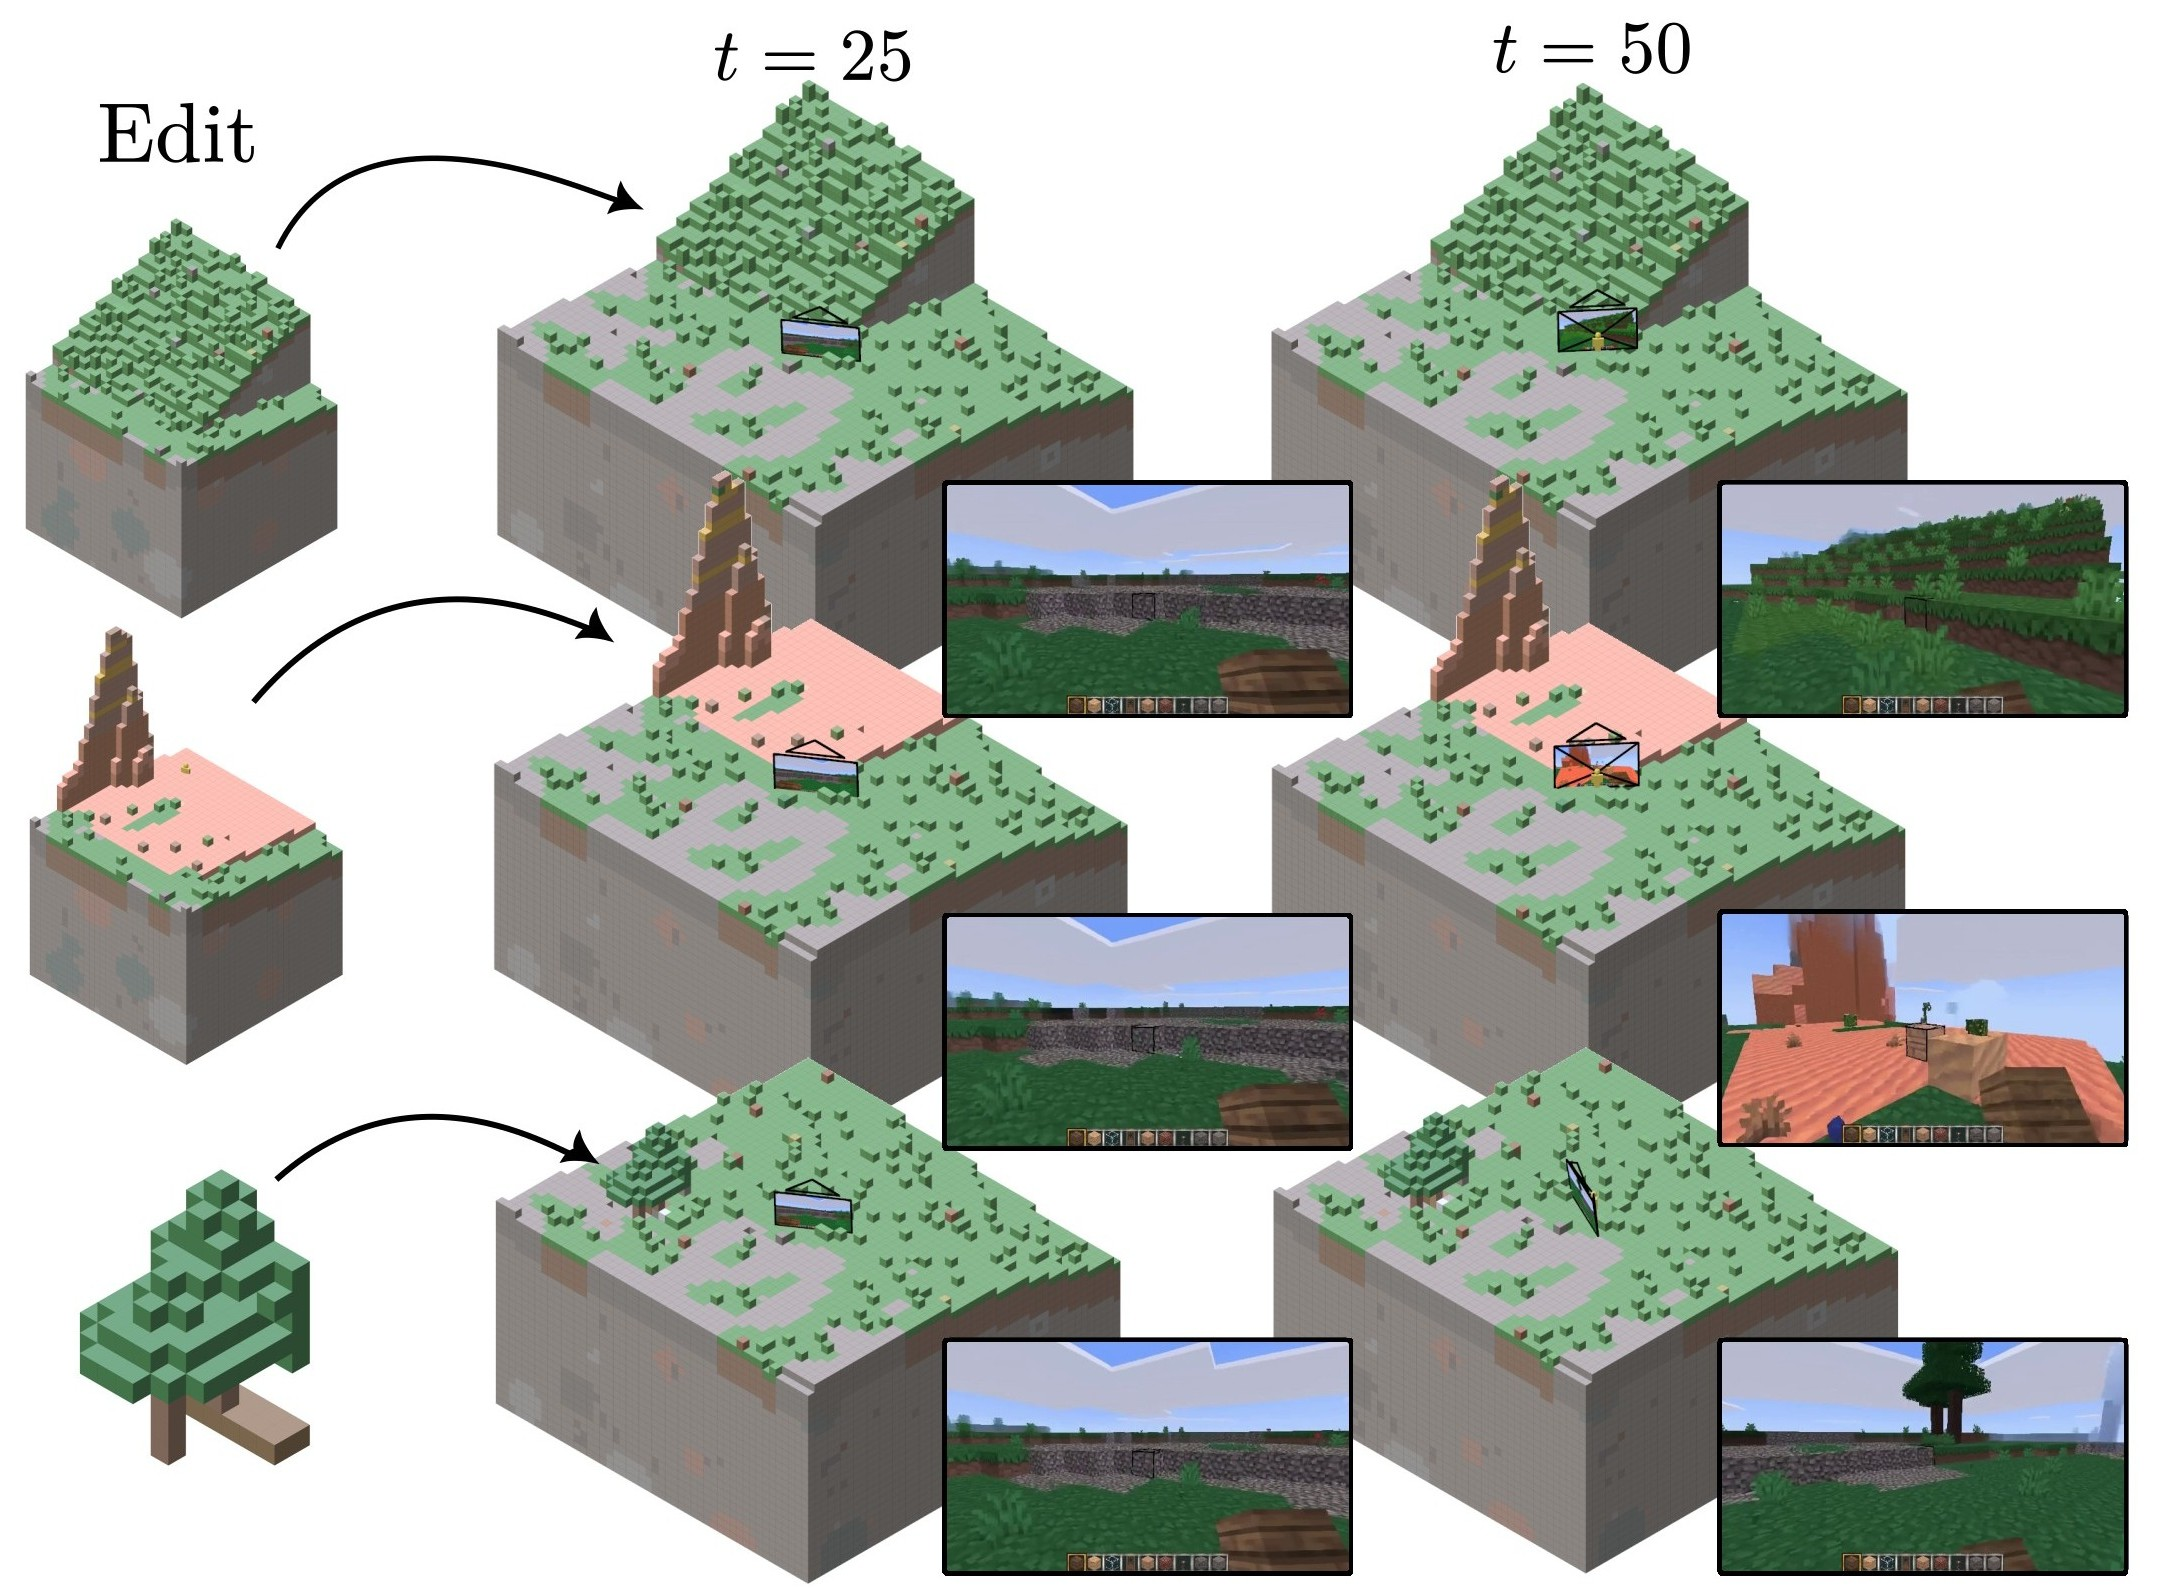
\includegraphics[width=1.04\linewidth]{figs/edits_single.jpg}}
    \caption{PERSIST's explicit 3D representation allows us to edit the world-state during an episode, enabling intuitive fine grained control over generations. We demonstrate this above with both global edits to terrain and biome, as well as the placement of smaller assets such as trees.}
    \label{c4:fig:voxel-edits}
     \vspace{-0.3cm}
  \end{center}
\end{figure}
%
% [cam-ready: see where to reinclude this]
%We craft action policies specifically designed to make the agent explore its environment while continually revisiting previously rendered locations at different times and from various viewpoints. We deploy these policies in Craftium to collect a dataset of evaluation trajectories. Finally, we sample starting conditions $\langle \vo_0, \vc_0\rangle$ and action sequences from the evaluation set to generate trajectories with PERSIST-S (featuring the 3D-S denoiser) and PERSIST (featuring the 3D-XL denoiser).
%As these methods were trained using Minecraft data, we collect a separate evaluation set in Minedojo~\citep{fan2022minedojo} to not induce domain shift, and we replicate their respective inference configurations.

%[cam-ready: very important include in caption of new figure]
%In the case of WorldMem, this includes initialising the memory bank used to sample key-frames with hundreds of ground truth cameras and pixel observations. This contrasts with PERSIST, which is initialised from a single initial frame $\langle \vo_0, \vc_0 \rangle$.

\begin{figure}[h]
  \begin{center}
    \centerline{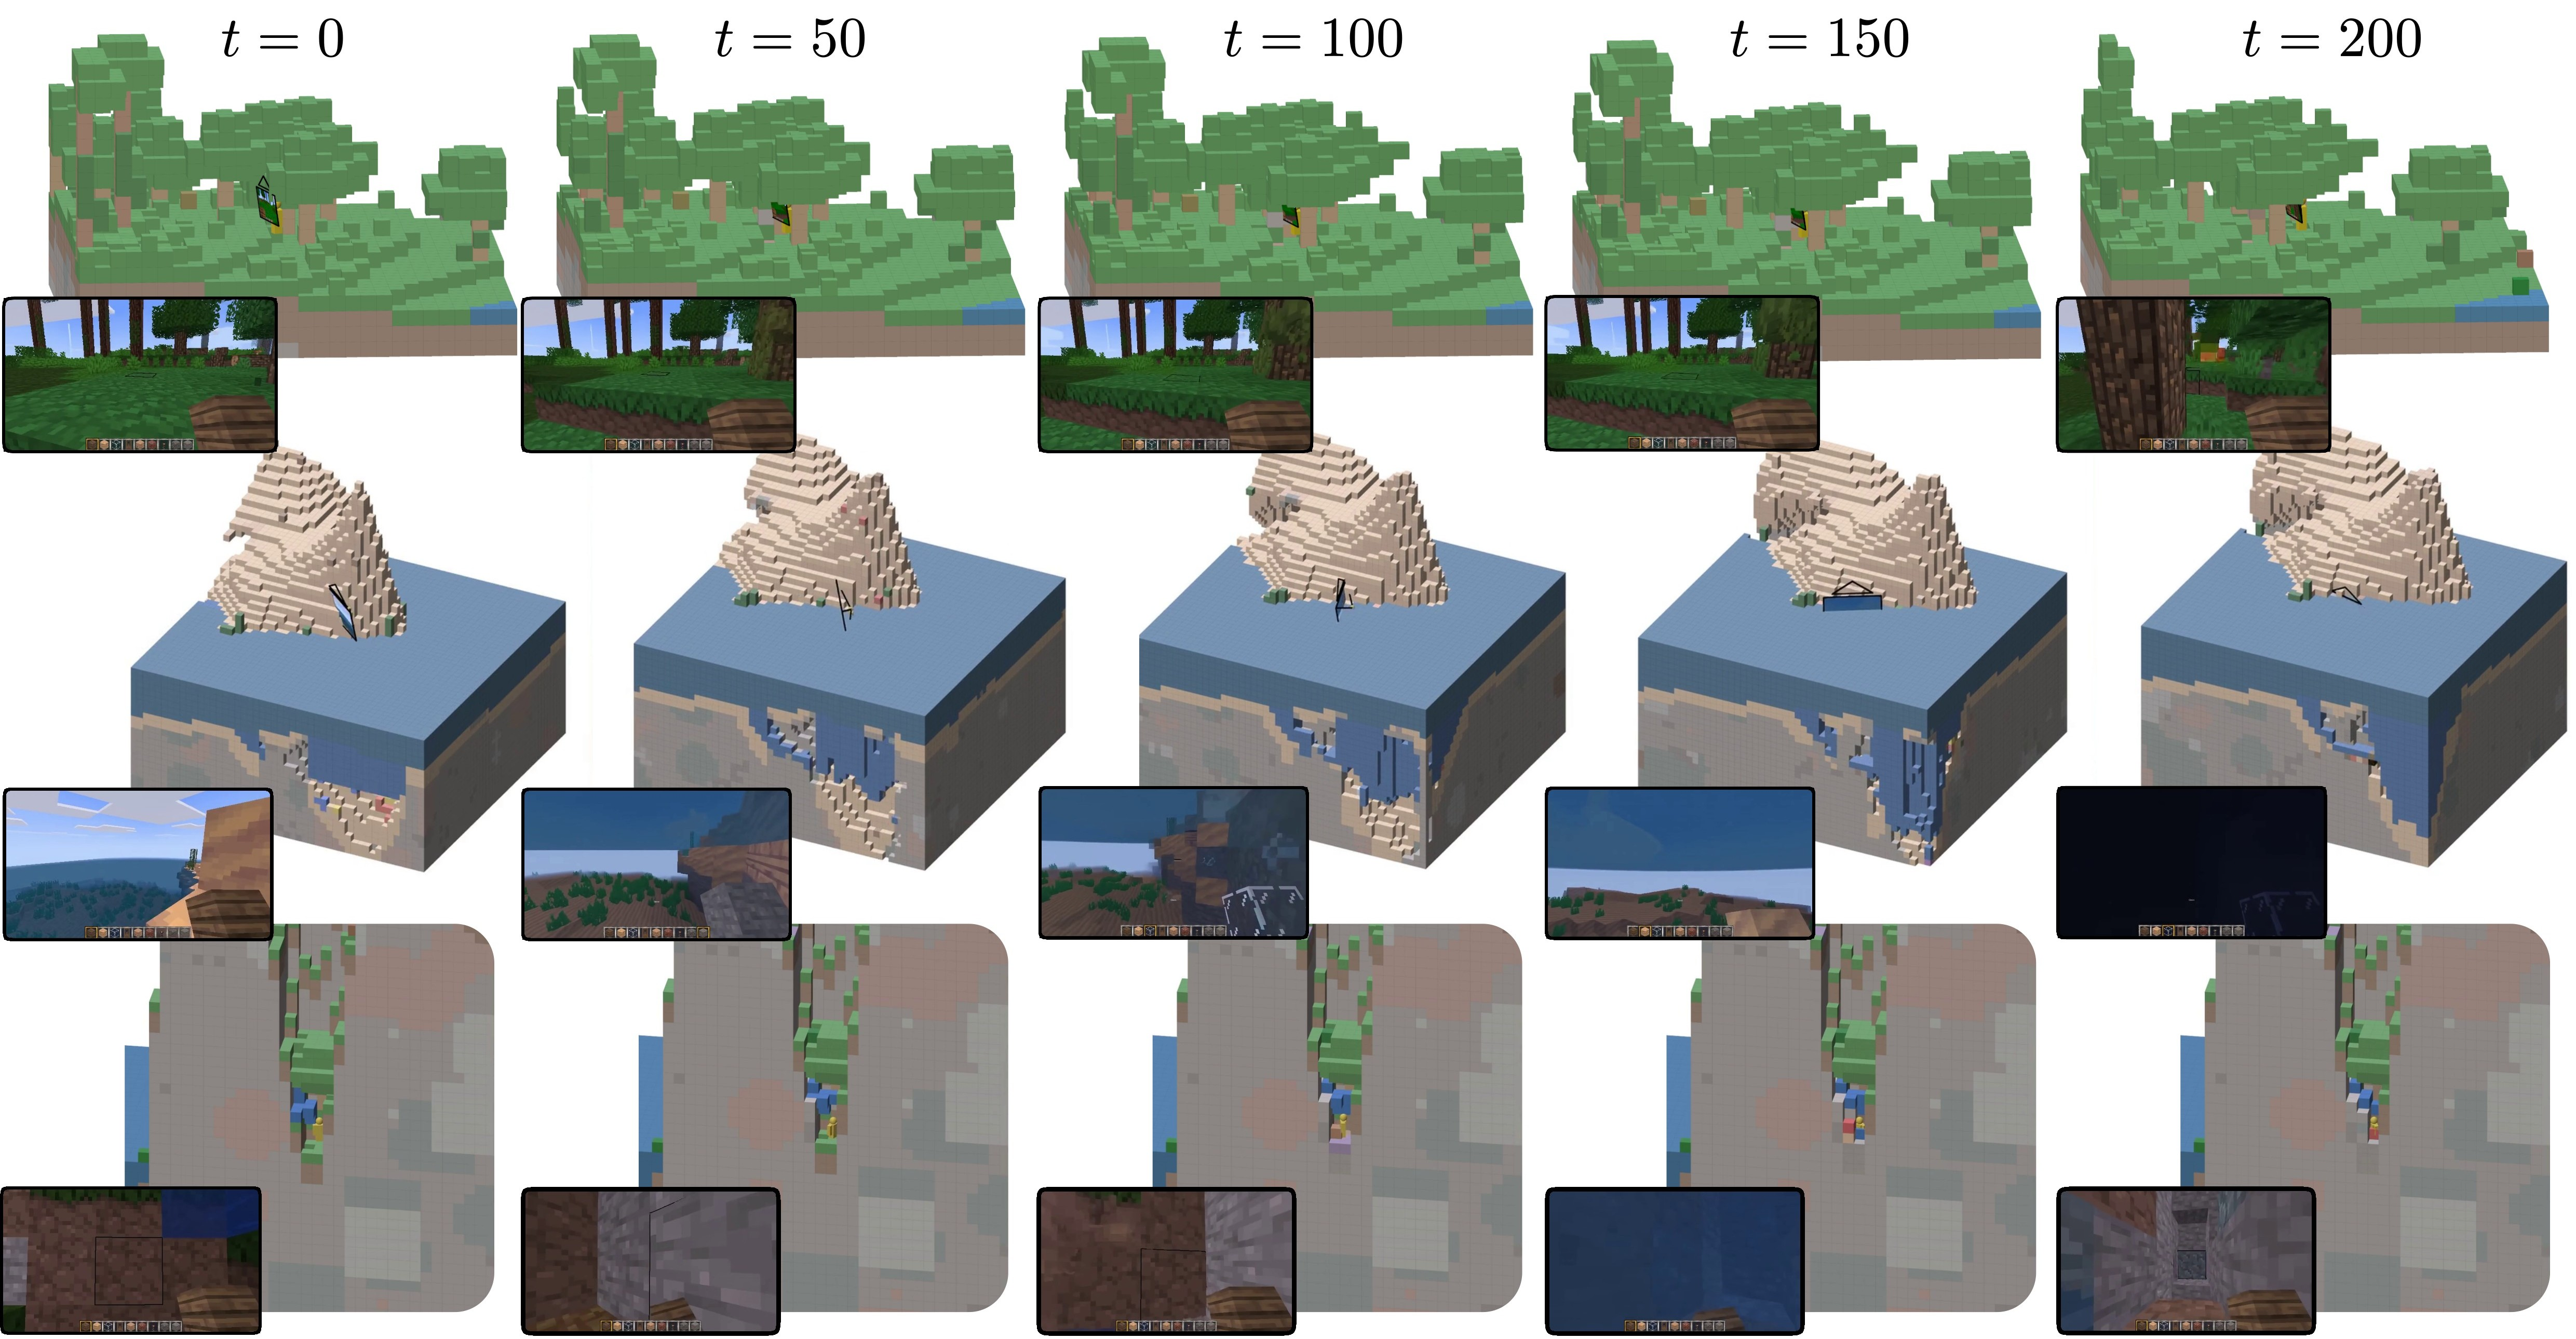
\includegraphics[width=1\linewidth]{figs/dynamic.jpg}}
    \caption{PERSIST's 3D state enables collision modelling with out-of-view elements (top: player moves backwards into a tree at $t=50$). Since the 3D state is dynamic, it evolves even when unobserved (middle: a cave filling with water). This allows off-screen events to produce emergent on-screen effects (bottom: water flowing onto the player at $t=150$).}
    \label{c4:fig:dynamic}
     \vspace{-0.7cm}
  \end{center}
\end{figure}


\subsection{Interactive Generation}

In this section, we evaluate our method's ability to generate spatially and temporally consistent interactive experiences within game worlds held out from the training set.

\textbf{Baselines.} We compare our approach with Oasis~\citep{decart2024oasis} and WorldMem~\citep{xiao2025worldmem}, two interactive video generation methods employing the same DiT backbone as $\gP_\theta$. WorldMem tracks camera states during the rollout and guides generation by retrieving key-frames from $O^{t-1}_0$ that closely match the current camera state. Oasis directly conditions on a sliding window of the most recent $K$ observations.

\textbf{Ablations.} We conduct several ablations to evaluate the core components and design choices of our method. Unless otherwise specified, our base configuration and all ablations utilize the 3D-XL denoiser.
\begin{itemize}[leftmargin=*,nosep]
\item \textbf{PERSIST-S} employs the smaller 3D-S denoiser to measure how an $8\times$ reduction in spatial tokens impacts the modeling capabilities of $\gW_\theta$.
\item \textbf{No-3D-Upscale} skips the 3D-VAE enhancement, projecting the world-frame latents directly into screen space without upscaling them to their native 3D resolution.
\item \textbf{Camera-GT} bypasses our learned camera model by conditioning directly on the ground-truth cameras.
\end{itemize}
Finally, we note that Oasis effectively serves as a baseline ablation of the entire 3D conditioning mechanism.

\textbf{Evaluation Setup.} To ensure a fair comparison, all baselines and ablations utilize the same VAEs and are trained under an identical rectified flow formulation on the training set. We measure the Fréchet Video Distance (FVD)~\citep{unterthiner2018towards} across 168 evaluation trajectories collected from held-out game worlds. These trajectories are generated using an action policy designed to balance world exploration with revisiting previously rendered locations from new viewpoints. \Cref{c4:tab:fvd} reports FVD scores computed over sets spanning the first 200, 400, and 600 trajectory timesteps. We use the first 400 ground truth frames and cameras to initialise WorldMem's memory bank. This contrasts with PERSIST, which only requires a single initial frame $\langle \vo_0, \vc_0 \rangle$.

\textbf{Quantitative Results.} As shown in \Cref{c4:tab:fvd}, baselines relying solely on pixel history (Oasis and WorldMem) yield significantly worse FVD scores, with generation quality degrading sharply over time. In contrast, PERSIST and its variants maintain stable FVD scores across extended horizons, highlighting the critical role of conditioning on the 3D state. Among the ablations, No-3D-Upscale suffers the highest FVD penalty. This confirms the benefit of rendering from a high-resolution 3D latent, which produces a $\vw_{2D}$ with superior depth resolution and 3D-to-pixel alignment. Conversely, PERSIST-S performs only marginally worse than the base configuration. While upscaling is crucial for rendering, the underlying 3D representation is highly robust to spatial compression (up to $512\times$ when combining the 3D-VAE and 3D-S denoiser). Finally, while Camera-GT achieves an FVD nearly identical to the base model, we observe that bypassing the learned camera model introduces physical inconsistencies that are not captured by the FVD (e.g. agent phasing through terrain or floating). We provide a qualitative example in \Cref{c4:fig:camera_clip}.

\textbf{Generation stability.} Qualitative analysis of sample rollouts (\Cref{c4:fig:rollout}) confirms that pixel-history baselines consistently produce irrecoverable artifacts by the 200\textsuperscript{th} timestep. In contrast, PERSIST produces remarkably stable rollouts. We corroborate this observation by measuring FID~\citep{heusel2017gans} at each generation timestep (\Cref{c4:fig:fid_vs_t}), finding that PERSIST suffers virtually no degradation over a 600-step episode. PERSIST does begin the episode with a slightly higher FID because it regenerates the initial pixel observation to ensure proper pixel/world-frame alignment. To demonstrate that this initial penalty is strictly an alignment artifact, \Cref{c4:fig:fid_vs_t} includes PERSIST$+\vw_0$, a variant introduced in \Cref{c4:sec:new_app} that receives perfectly aligned initial world and pixel frames. Regardless of initialization, PERSIST maintains its visual quality over time, whereas pixel-history baselines rapidly degrade.

In practice, we observe that the world-frames produced by $\gW_\theta$ remain coherent for several thousand steps. Because $\vw_{2D}$ is obtained directly from these highly stable world-frames, it provides reliable structural guidance over long horizons and lets $\gP_\theta$ recover from visual artifacts. We showcase multiple examples of this self-correction over the course of a 2,000-step episode in \Cref{c4:fig:limitations}.

\textbf{Human study.} While FVD and FID scores capture distribution-level discrepancies, they are known to favor per-frame visual quality over the spatial and temporal coherence of individual generations \citep{ge2024content}. To complement our automated metrics, we conduct a human study comprising over 800 rollout evaluations from 28 participants. Users rated each video on ``Visual Fidelity'', ``3D Consistency'' and ``Temporal Consistency'', before assigning an overall score. Results are summarized in \Cref{c4:tab:eval}, with full methodological details in \Cref{c4:app:data_met} and extended results in \Cref{c4:app:ext_user_study}. Across all metrics, PERSIST configurations consistently outperform the baselines, corroborating our quantitative and qualitative findings. Interestingly, PERSIST-S performs similarly to the base configuration in both average user ratings and head-to-head comparisons. This highlights that the FVD penalty observed for PERSIST-S does not translate to a human-perceptible degradation in generation quality.

\textbf{Inference efficiency.} Finally, we conduct a preliminary investigation into the speed-quality tradeoff of our method. We find that generation stability is preserved even when reducing the number of denoising steps from 20 down to 2 and 4 for $\gW_\theta$ and $\gP_\theta$, respectively. This yields a $3\times$ inference speed-up with only a moderate impact on generation quality (see \Cref{c4:app:speed} for a detailed analysis).

%todo Add this again if head to head comparison is good. indicating that increasing the capacity of the 3D representation translates directly into stronger world modelling performance

% Notes on eval set:
% - describe eval set, make distinction between two type of trajectories: 
%        - Orbit: specifically designed to challenge spatial +  temporal consistency (spatial: viewing object/scenes from different view points, temporal: revisiting already explored locations/views)
%        - Free-Play: Agent perform randomised actions in the environment
%        - Exploration: Actions are aimed to cover a large distance (more timesteps, agent moves forward/backward and spins on itself periodically)


% Notes on Baselines:
% - describe baselines and highlight inherent limitations: e.g. Oasis/Mineworld have no memory mechanism (but Oasis uses 2x temporal context window as our models). WorldMem/MemoryForcing require hundred of GT frame to be warm-started at inference.
% - mention a separate eval set is collected in MineDojo to not induce domain shift for baselines.
% - mention our training set if much smaller than VPT training set (check size but I think 10-100x smaller

\subsection{New Applications and Emerging Capabilities}\label{c4:sec:new_app}

% \begin{figure}[ht]
%   \begin{center}
%     \centerline{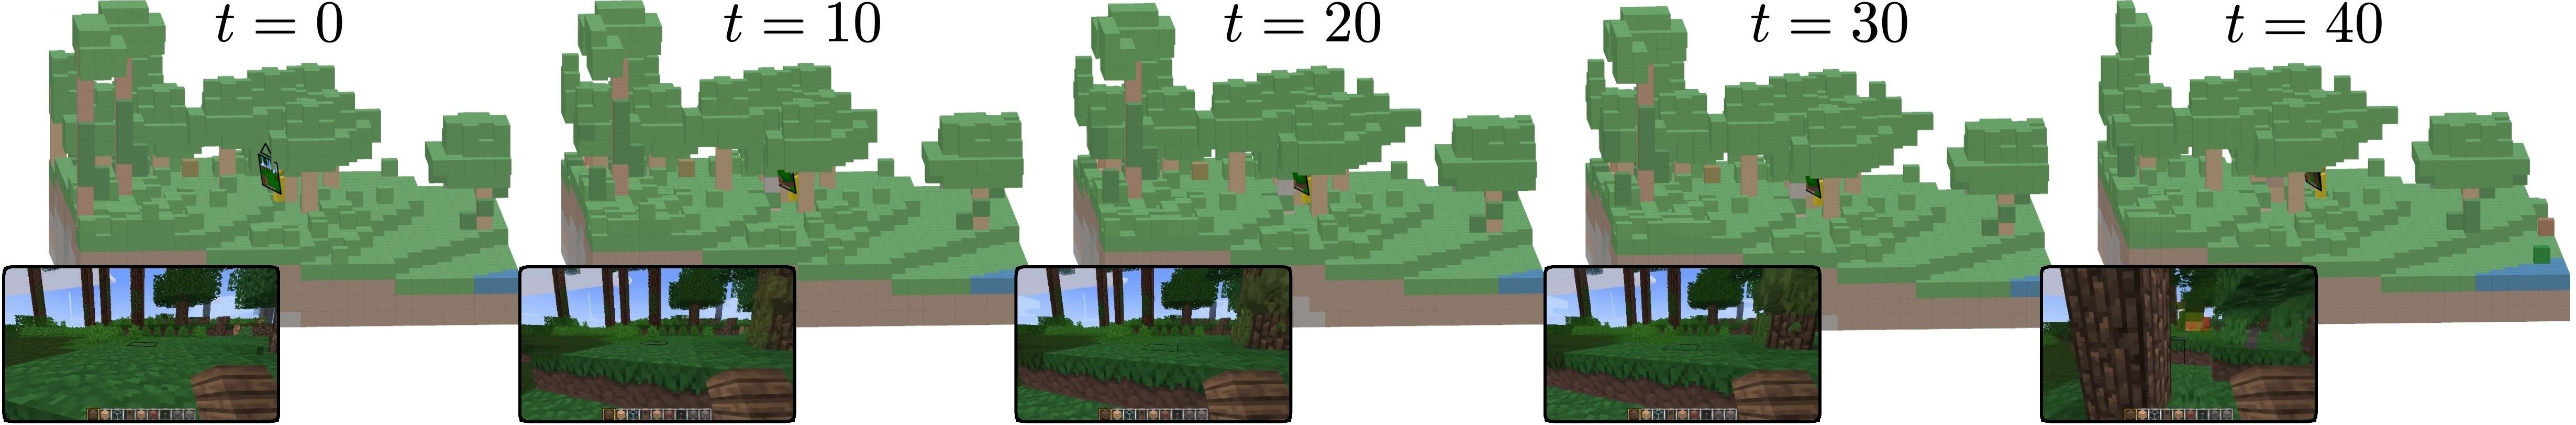
\includegraphics[width=\linewidth]{figs/collision.jpg}}
%     \caption{PERSIST captures challenging physical interactions, such as a collisions with out of view elements (tree at $t=10$)}
%     \label{c4:fig:collision}
%      \vspace{-0.2cm}
%   \end{center}
% \end{figure}

In addition to its improvement to the quality and coherence of generated experiences, we find that PERSIST's 3D representation confers a number of new capabilities.

\textbf{3D generation.} At initialisation, it is essential for $\vw_0$ to capture the structure and semantics of the provided conditioning RGB observation. In \Cref{c4:fig:w0_gen}, we show that $\gW_\theta$ successfully generates plausible starting world frames, while also outpainting unseen regions differently from one episode to the next. This ability lets PERSIST generate environments that are both diverse and coherent, supporting a wide variety of interactive experiences.

%Todo: example
\textbf{Explicit 3D initialisation.} By default, PERSIST initialises generation from starting condition $\langle \vo_0, \vc_0\rangle$, with the initial world-frame $\vw_0$ being inferred by the world dynamics model $\gW_\theta$. However, PERSIST also supports $\vw_0$ being provided as a starting condition\footnote{See \Cref{c4:alg:PERSIST,c4:alg:PERSIST-w0} for the respective inference algorithms of PERSIST and PERSIST+$\vw_0$.}. This explicit 3D conditioning allows a greater degree of control over the generated experience than providing an image, as the full surroundings of the agent can be specified.


To assess how effectively PERSIST can leverage explicit 3D conditioning, we evaluate a variant denoted PERSIST+$\vw_0$, where a ground-truth world-frame $\vw_0$ is provided at initialisation. PERSIST+$\vw_0$ achieves lower FID and FVD scores and higher human ratings (\Cref{c4:tab:fvd,c4:tab:eval}, \Cref{c4:fig:fid_vs_t}), demonstrating that the model successfully incorporates the additional information contained within $\vw_0$. % COMMENTED BECAUSE NO LONGER TRUE WITH LARGER HUMAN STUDY Notably, PERSIST and PERSIST+$\vw_0$ achieve similar human ratings. Here, FVD gains primarily reflect how additional information about the environment's initial state brings closer alignment with the evaluation videos. However there is no perceptible impact to the consistency or the quality of individual experiences when this information is not available, as PERSIST successfully extrapolates from $\langle \vo_0, \vc_0\rangle$ to generate a coherent 3D environment.

\textbf{World edits mid-generation.} \citet{valevski2024diffusionmodelsrealtimegame} and \citet{kanervisto2025world} proposed to perform manual edits to generated pixel frames before re-injecting them as context, as an alternative way of controlling the generated experience. As we can extract $\vw_t$ at any point during generation, we obtain the capability of making precise 3D-edits to the world mid-episode. We pause generation at timestep $t$ and manually edit $\vw_t$ to obtain $\tilde{\vw}_t$. We then restart generation using $\{\tilde{\vw}_t, \vc_t, \vo_t, \va_t\}$ as the starting condition. We show several edit examples in \Cref{c4:fig:voxel-edits}. 

\textbf{Persistent world dynamics.} PERSIST learns to model environmental processes that evolve on their own. In \Cref{c4:fig:dynamic}, we provide examples of environment dynamics and interactions occurring outside of the agent's view. We observe that dynamics occurring off-screen will sometimes act as causal drivers for emergent on-screen effects.

%PERSIST continuously models dynamic processes in the environment, even while they are not being actively rendered to screen space. In \Cref{c4:dynamic}, we observe a waterfall gradually flooding the area, causing some water to eventually appear in the player's view.
\vspace{-0.25cm}
\section{Conclusion}
\vspace{-0.22cm}
In this work, we introduced PERSIST, a world modelling framework that tracks the evolution of a persistent latent 3D state. Our results demonstrate that actively generating guidance frames from this 3D state substantially improves spatial memory, temporal coherence, and overall generation quality and stability compared to conditioning on pixel-based histories. We show that tracking this 3D world state allows the model to capture environment dynamics occurring beyond the agent's view. Additionally, it lets users pre-specify, visualise, and modify the structure of generated environments, creating new ways of controlling generated experiences.

Despite these advances, PERSIST currently relies on ground-truth 3D supervision during training and maintains a finite region of 3D space in memory. Furthermore, our implementation was not optimised for inference speed and does not yet achieve real-time inference. We believe these limitations outline a clear roadmap for future research involving persistent 3D world states: in-the-wild training via synthetic 3D annotations obtained from 2D-to-3D foundation models~\citep{wang2025vggt,sam3dteam2025sam3d3dfyimages}, end-to-end post-training on generated rollouts to mitigate autoregressive drift~\citep{huang2025self}, and access to unconstrained spatial memory via a 3D memory bank. We provide a detailed discussion of these directions in Appendix~\ref{c4:app:limitations}.

\section*{Impact Statement}

This work advances the field of Machine Learning by improving the spatial and temporal consistency of generative world models.
While our research is primarily conducted within the simulated environment of Luanti, the underlying methodologies have potential applications in video games, digital twin simulation, and embodied AI navigation, where reliable 3D scene representation is critical.
We do not foresee any immediate negative societal consequences that require specific highlighting at this stage, as our model operates within a synthetic domain.

% In the unusual situation where you want a paper to appear in the
% references without citing it in the main text, use \nocite
% \nocite{langley00}

%% (references resolve against the global thesis bibliography)

%%%%%%%%%%%%%%%%%%%%%%%%%%%%%%%%%%%%%%%%%%%%%%%%%%%%%%%%%%%%%%%%%%%%%%%%%%%%%%%
%%%%%%%%%%%%%%%%%%%%%%%%%%%%%%%%%%%%%%%%%%%%%%%%%%%%%%%%%%%%%%%%%%%%%%%%%%%%%%%
% APPENDIX
%%%%%%%%%%%%%%%%%%%%%%%%%%%%%%%%%%%%%%%%%%%%%%%%%%%%%%%%%%%%%%%%%%%%%%%%%%%%%%%
%%%%%%%%%%%%%%%%%%%%%%%%%%%%%%%%%%%%%%%%%%%%%%%%%%%%%%%%%%%%%%%%%%%%%%%%%%%%%%%
%% --- Appendix: rendered as per-chapter lettered sections (A, B, ...) ---
\clearpage
\begin{subappendices}
\crefalias{section}{appendix}
\crefalias{subsection}{appendix}

\section{Additional Implementation Details}\label{c4:app:implt}


\subsection{Additional Model Details}

\textbf{2D VAE.} We employ a vision transformer architecture \cite{dosovitskiy2020image}, using the open-source implementation of \cite{decart2024oasis}. We train the VAE via an MSE reconstruction objective, alongside a KL divergence penalty coefficient of $1e-6$.

\textbf{3D VAE.} We employ a 3D-ResNet architecture based on the implementation provided by \cite{xiang2024structured}. We train the VAE via a cross-entropy loss to predict voxel class labels, alongside a KL divergence penalty coefficient of $1e-6$.

\textbf{Differentiable Rasterizer.} For our projecting function $\mathcal{R}$, we leverage GPU-native triangle rasterization, by assigning voxel features to faces of a static voxel-grid mesh. Then, depth-peeling~\cite{bavoil2008order, nagy2003depth} is applied during rasterization to produce a per-pixel, depth-ordered stack of 3D features $W_{2D}^{t} \in \mathbb{R}^{H \times W \times L \times C}$, where $L$ is the maximum number of layers. Since the mesh topology is fixed for a given resolution, we construct it once at initialisation, updating vertex attributes in-place to avoid redundant mesh construction.  

\subsection{PERSIST and PERSIST$+w_0$ Inference Logic}
We detail the inference procedures for PERSIST with and without 3D state $w_0$ initialization in
Algorithms~\ref{c4:alg:PERSIST} and~\ref{c4:alg:PERSIST-w0} respectively.

\subsection{Model and Inference Hyperparameters}
We summarize the model architectures and inference hyperparameters used in our system. Table~\ref{c4:table:w-vae} and Table~\ref{c4:table:p-vae} describe the configurations of the 3D-VAE and 2D-VAE respectively, while Table~\ref{c4:table:cam-model} details the camera model architecture. We further report the world and pixel denoiser configurations in Table~\ref{c4:table:world-denoiser} and Table~\ref{c4:table:pixel-denoiser}. Finally, Table~\ref{c4:table:samplers} summarizes inference-time sampling hyperparameters, and Table~\ref{c4:table:cam-model} lists token statistics across models.



\begin{table}[htbp]
\centering
\scriptsize
\setlength{\tabcolsep}{4pt}

\begin{minipage}[t]{0.48\textwidth}
\centering

\caption{3D-VAE configuration.}
\label{c4:table:w-vae}
\begin{tabular}{cc}\toprule
Parameter & Value \\
\midrule
input shape & [48, 48, 48, 2138] \\
number of residual blocks & 2 \\
middle channels & [32, 128, 512] \\
$\bar{w}$ shape & [12, 12, 12, 48] \\
\# parameters & 138M \\
\bottomrule
\end{tabular}

\vspace{0.8em}

\caption{2D-VAE configuration.}
\label{c4:table:p-vae}
\begin{tabular}{cc}\toprule
Parameter & Value \\
\midrule
input size & [360, 640, 3] \\
patch size & 10 \\
$\bar{o}$ shape & [36, 64, 16] \\
encoder dimension & 1024 \\
encoder depth & 6 \\
encoder number of heads & 6 \\
decoder dimension & 1024 \\
decoder depth & 12 \\
decoder number of heads & 16 \\
\# parameters & 227M \\
\bottomrule
\end{tabular}

\vspace{0.8em}

\caption{Camera model configuration.}
\label{c4:table:cam-model}
\begin{tabular}{cc}\toprule
Parameter & Value \\
\midrule
rotation embedding channels & 256 \\
translation embedding channels & 256 \\
hidden size & 1024 \\
transformer blocks & 12 \\
number of heads & 12 \\
MLP ratio & 4 \\
context window size & 8 \\
\# parameters & 234M \\
\bottomrule
\end{tabular}

\vspace{0.8em}

\caption{Number of spatial and temporal tokens for different models.}
\label{c4:table:tokens}
\begin{tabular}{lcc}
\toprule
Model & \# Temporal Tokens & \# Spatial Tokens \\
\midrule
$\gW_\theta$-S & 8 & 216 \\
$\gW_\theta$-XL & 8 & 1728 \\
$\gP_\theta$ & 16 & 576 \\
$\gC_\theta$ & 8 & n/a \\
\bottomrule
\end{tabular}

\end{minipage}
\hfill
\begin{minipage}[t]{0.48\textwidth}
\centering

\caption{World denoiser hyperparameters (3D-S configuration). The XL configuration uses patch size=1 and has the same number of learned parameters.}
\label{c4:table:world-denoiser}
\begin{tabular}{cc}\toprule
Parameter & Value \\
\midrule
input shape & [12, 12, 12, 48] \\
patch size & 2 \\
hidden size & 1024 \\
cross condition hidden size & 1024 \\
depth & 12 \\
number of heads & 16 \\
MLP ratio & 4 \\
pixel condition patch size & 2 \\
context window size & 8 \\
\# parameters & 686M \\
\bottomrule
\end{tabular}

\vspace{0.8em}

\caption{Pixel denoiser configuration.}
\label{c4:table:pixel-denoiser}
\begin{tabular}{cc}\toprule
Parameter & Value \\
\midrule
$\bar{o}$ shape & [36, 64, 16] \\
$\bar{o}$ embedder output channels & 16 \\
patch size & 2 \\
hidden size & 1024 \\
depth & 12 \\
number of heads & 16 \\
MLP ratio & 4 \\
$\tilde{w}_{2D}$ shape & [36, 64, 192, 32] \\
${w}_{2D}$ embedder patch size & 6 \\
${w}_{2D}$ embedder stride & 4 \\
${w}_{2D}$ embedder output channels & 752 \\
context window size & 16 \\
\# parameters & 460M \\
\bottomrule
\end{tabular}

\vspace{0.8em}

\caption{Flow matching sampler configurations at inference time.}
\label{c4:table:samplers}
\begin{adjustbox}{max width=\linewidth}
\begin{tabular}{cc}\toprule
Parameter & Value \\
\midrule
minimum noise $\sigma_\text{min}$ & $1e-5$ \\
denoising steps & 20 \\
denoising step scheduling function & $\tau^k = \frac{\eta k}{1 + (\eta-1)k}$ \\
$\eta$ & 3 \\
noise level applied to context (past) frames $\tau_\text{ctx}$ & 0.02 ($\gW_\theta$) / 0.1 ($\gP_\theta$) \\
\bottomrule
\end{tabular}
\end{adjustbox}

\end{minipage}

\end{table}



%\clearpage

\section{Evaluation Methodology}\label{c4:app:data_met}

% \subsection{Training data}
% \todo[inline]{
% \begin{enumerate}
%     \item What policy was used? Describe action groups
%     \item Mention how long it takes to collect dataset
%     \item Any other important details?
% \end{enumerate}
% }

\subsection{Quantitative analysis}

We collect a total of 168 rollouts of 600 frames for each method. We then compute FVD and FID scores from the latent features obtained by passing rollout and ground truth clips through a pretrained Inflated 3D ConvNet \citep{carreira2017quo}. We compute FID scores at each timestep, whereas we compute the FVD by splicing rollouts into 16-frame clips, discarding leftover frames.

\subsection{Human Study Data}

For the human study, we collected evaluation datasets across four hand-crafted policies: \textit{Free Play}, \textit{Move Forward}, \textit{Move Backward}, and \textit{Orbit}.
These policies are designed to produce trajectories that require a high level of temporal and spatial consistency to be correctly simulated by the world model.

\begin{itemize}
    \item \textbf{Free Play:} randomly samples action from a set of pre-defined sequences, facilitating exploration.
    \item \textbf{Move Forward/Backward:} The agent moves forwards or backwards, periodically spinning on itself to observe its surroundings.
    \item \textbf{Orbit:} The agent follows a circular trajectory, while constantly adjusting its heading to look towards the centre of the circle.
\end{itemize}

%We craft action policies specifically designed to make the agent explore its environment while continually revisiting previously rendered locations at different times and from various viewpoints. We deploy these policies in Craftium to collect a dataset of evaluation trajectories. Finally, we sample starting conditions $\langle \vo_0, \vc_0\rangle$ and action sequences from the evaluation set to generate trajectories with PERSIST-S (featuring the 3D-S denoiser) and PERSIST (featuring the 3D-XL denoiser).
%As these methods were trained using Minecraft data, we collect a separate evaluation set in Minedojo~\citep{fan2022minedojo} to not induce domain shift, and we replicate their respective inference configurations.

For the human study, we evaluated the models released by the original authors, as we conducted it prior to training Oasis and WorldMem models on our training set. As these methods were trained using Minecraft data, we collected separate evaluation sets in Minedojo~\citep{fan2022minedojo} to not induce domain shift, and we replicated their respective inference configurations. In the case of WorldMem, this included initialising the memory bank used to sample key-frames with 600 ground truth cameras and pixel observations. To ensure this difference in domains did not bias human ratings, we compared ratings of ground-truth videos from both sets. We observed no significant preference for either domain, with a difference in average scores of less than 0.15 (3.75\%).

\subsection{Human Study Protocol}\label{c4:app:method_user_study}
The user study was deployed via a custom web interface (see Figure~\ref{c4:fig:ui_screenshot}). Participants were tasked with scoring videos according to the following metrics and instructions:
\begin{itemize}
    \item \textbf{Visual Fidelity.} Per-frame visual quality of the video. Deduct points for visual artifacts such as blurriness, color shifts, flickering, noise, or texture degradation.
    \item \textbf{3D Spatial Consistency.} Spatial consistency of the scene. Deduct points if objects deform, shift, or change appearance when viewed from different camera angles, or if the relative depth and spatial relationships between objects appear inconsistent as the player moves.
    \item \textbf{Temporal Environment Stability and Consistency.} Consistency of the environment over time. Deduct points if the scene changes unexpectedly, such as objects disappearing, reappearing, or changing structure when revisiting previously seen areas, or if the environment degrades or becomes unnaturally simplified over time.
    \item \textbf{Overall Quality Score.} Your subjective rating of the overall quality of the video, considering all factors above.
\end{itemize}
Ratings had the range of 1-5. Videos were presented to the user as pairs. Each pair depicted matching behaviour (free play, move forward, move backward, orbit) but different methods (baselines, PERSIST configurations, Minedojo or Craftium ground truth). Each individual user was asked to rate up to 50 videos. User assessments were subsequently aggregated to compute average scores. We consider the first three evaluation trials for each participant to count as calibration, and we discard them from the study.

Overall, a total of 28 participants evaluated over 800 videos. 93\% of study participants were AI/ML practitioners and mostly active gamers (48\% casual, 41\% regular). 17\% of active gamers had over 100 hours of playtime on Minecraft, 21\% had played 10–100 hours and 28\% had under 10 hours. 35\% had heard of Minecraft but had never played.

\begin{figure}[ht]
    \centering
    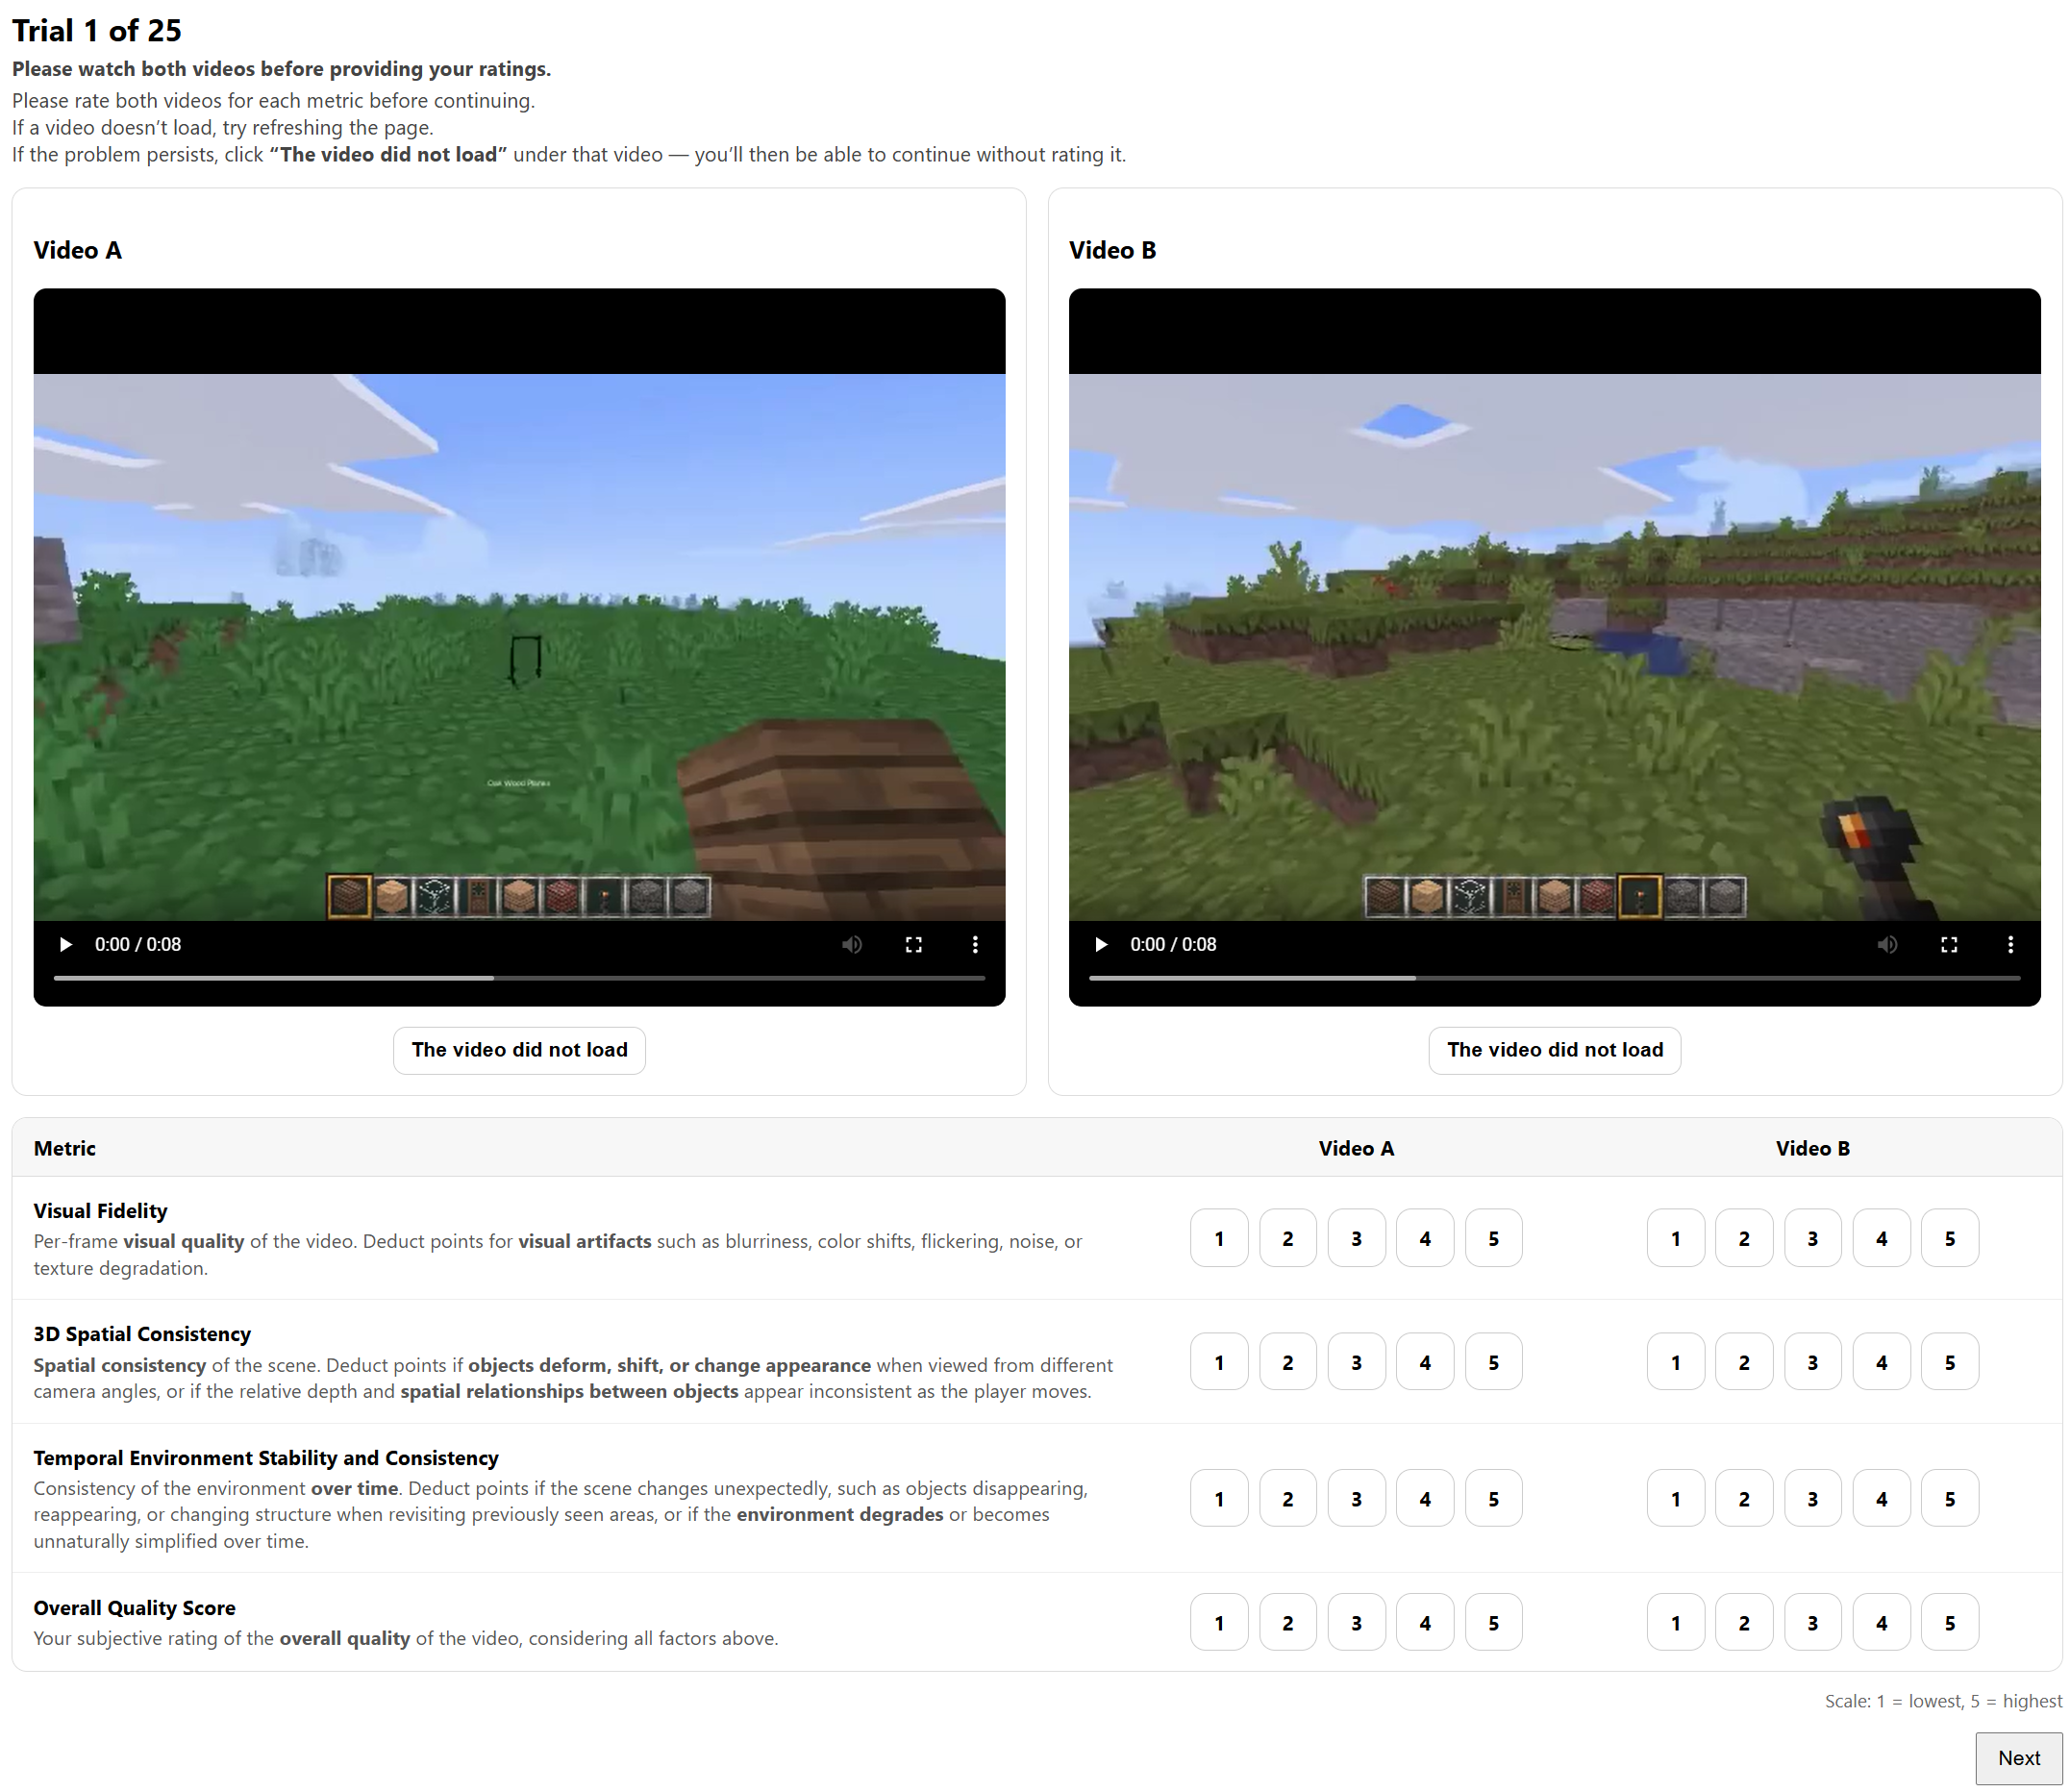
\includegraphics[width=1.0\linewidth]{figs/UI.png}
    \caption{\textbf{User Study Interface.} A screenshot of our web-based platform where participants evaluate video pairs based on temporal and spatial consistency.}
    \label{c4:fig:ui_screenshot}
\end{figure}

\section{Extended User Study Results}\label{c4:app:ext_user_study}

\subsection{Score Differences During Head-to-Head Comparisons}
Given that users rate two side-by-side videos during each trial, we can analyse how our default configuration fares in a direct head-to-head comparison against any other baseline, PERSIST configuration, or the ground truth data. We provide score comparison matrices below (one per metric) displaying the average score deltas during head-to-head comparisons.

PERSIST configurations consistently outperform the baselines in every head-to-head comparison. During head-to-head comparisons between PERSIST-S and the default configuration, PERSIST-S narrowly wins on 3D Spatial Consistency ($+0.21$), while the default configuration achieves a slightly higher Overall Quality Score ($+0.14$). The differences in Visual Fidelity and Temporal Consistency are too narrow to call for either side. While the default configuration achieves a better FVD, the results of the study indicate that humans do not observe a significant performance degradation when we decrease the number of spatial tokens allotted to $\gW_\theta$. In contrast, PERSIST$+\vw_0$ wins most head-to-head comparisons against base and PERSIST-S, which indicates that providing direct 3D conditioning generally improves performance. 

Finally, users consistently prefer ground-truth videos across all metrics, highlighting that even our strongest configurations remain below the quality of real trajectories. This persistent gap underscores both the difficulty of long-horizon world modelling with procedurally generated environments, and the opportunity for further advances in persistent 3D generative representations.
\begin{figure}[!htb]
    \centering

    \begin{subfigure}{0.48\linewidth}
        \centering
        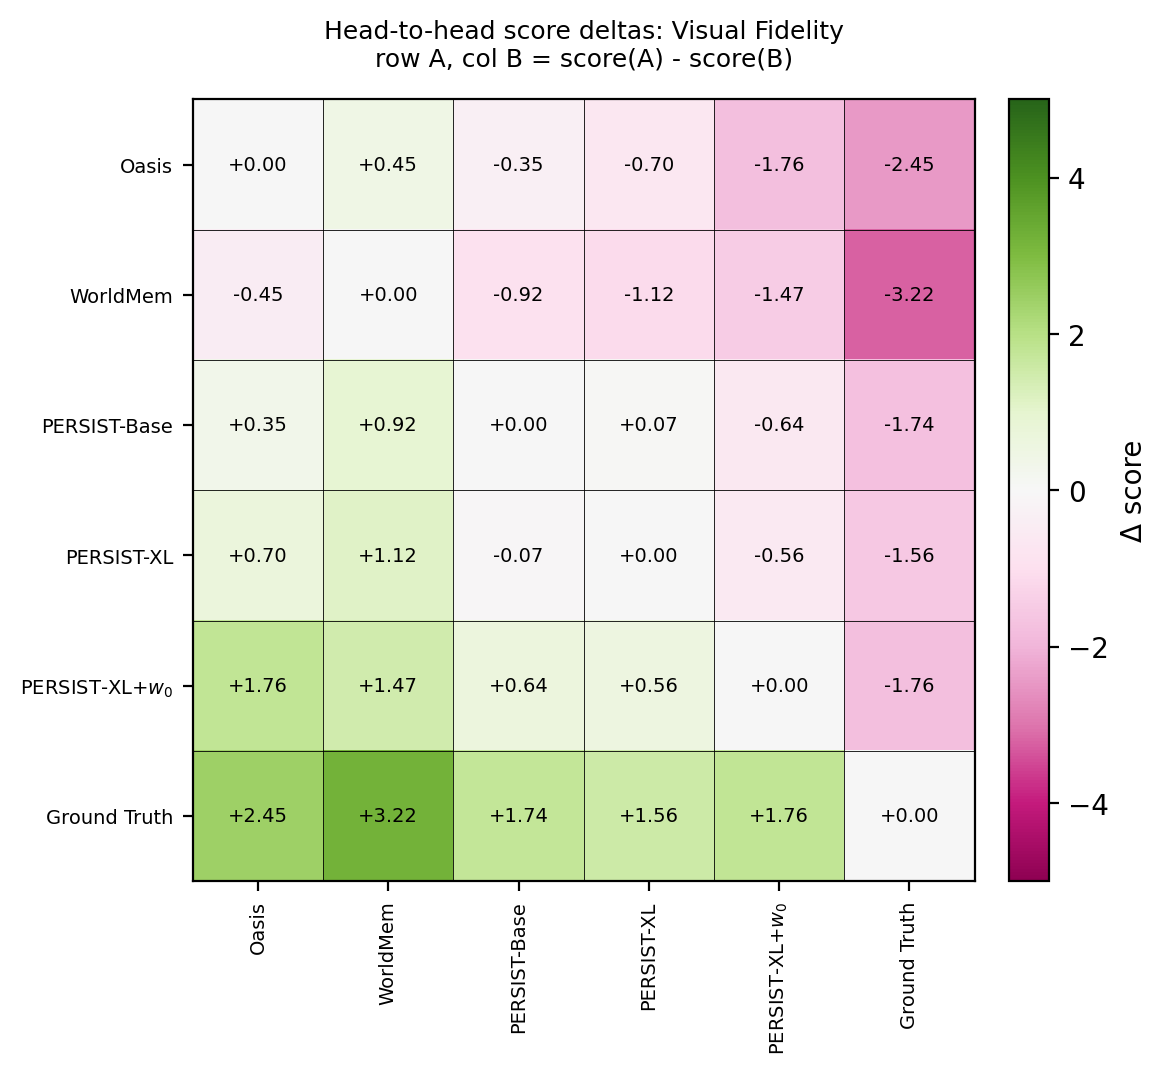
\includegraphics[width=\linewidth]{figs/h2h_png/h2h_metric_a.png}
        \caption{\textbf{Visual fidelity}}
        \label{c4:fig:hth_a}
    \end{subfigure}
    \hfill
    \begin{subfigure}{0.48\linewidth}
        \centering
        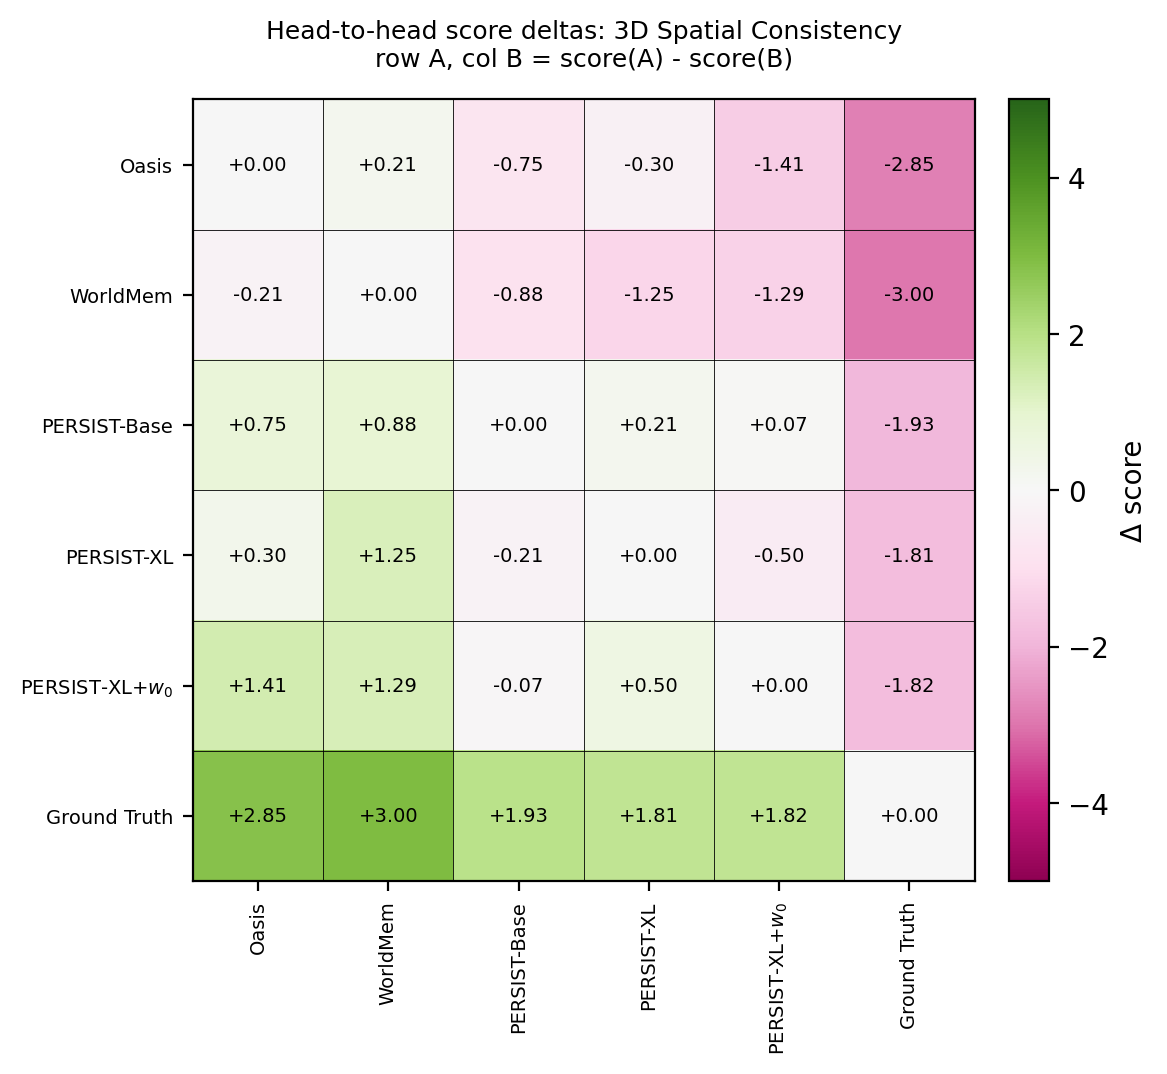
\includegraphics[width=\linewidth]{figs/h2h_png/h2h_metric_b.png}
        \caption{\textbf{3D spatial consistency}}
        \label{c4:fig:hth_b}
    \end{subfigure}

    \vspace{0.5em}

    \begin{subfigure}{0.48\linewidth}
        \centering
        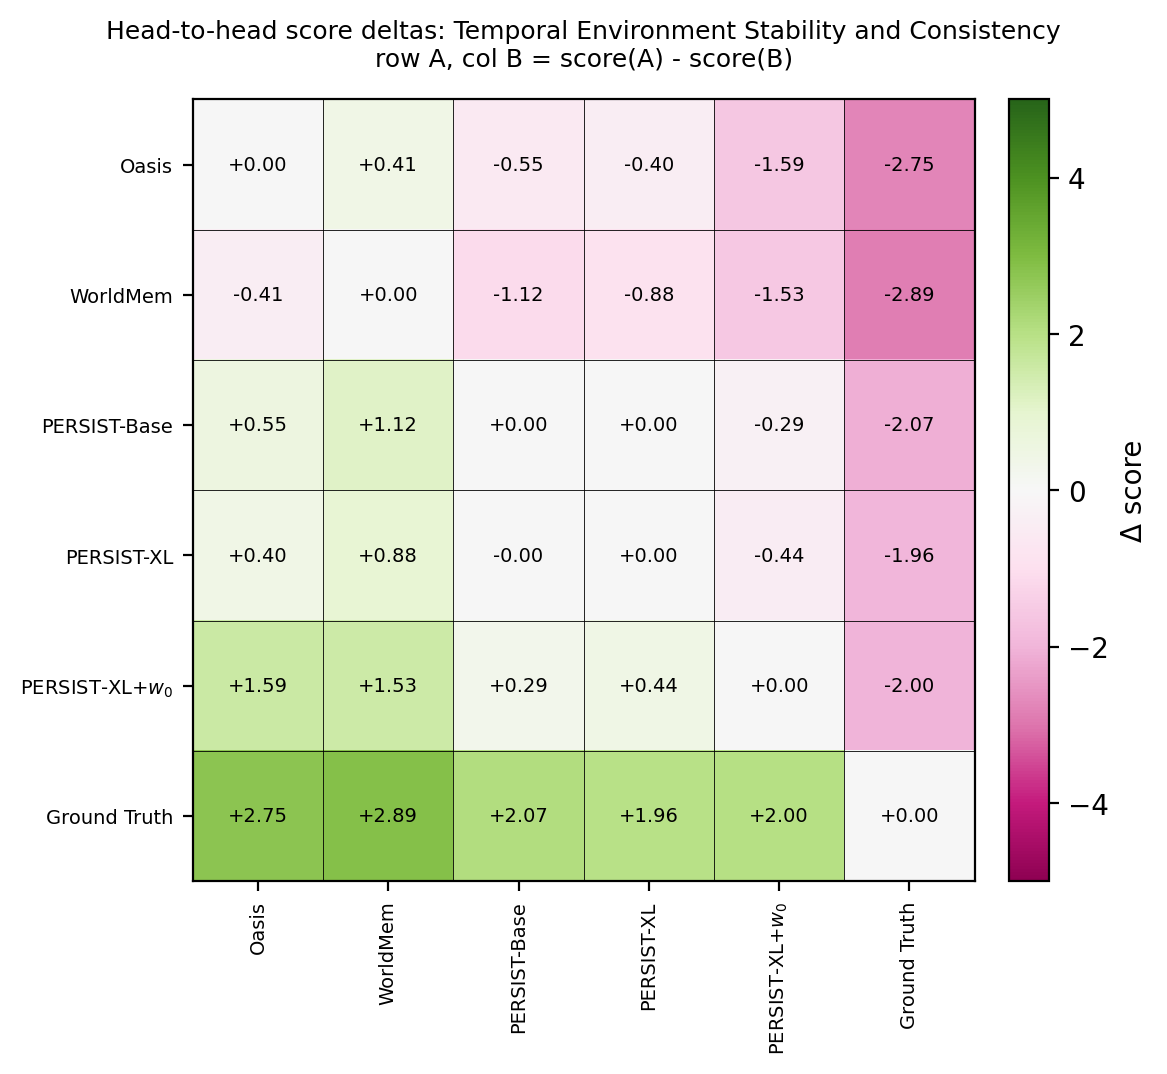
\includegraphics[width=\linewidth]{figs/h2h_png/h2h_metric_c.png}
        \caption{\textbf{Temporal consistency}}
        \label{c4:fig:hth_c}
    \end{subfigure}
    \hfill
    \begin{subfigure}{0.48\linewidth}
        \centering
        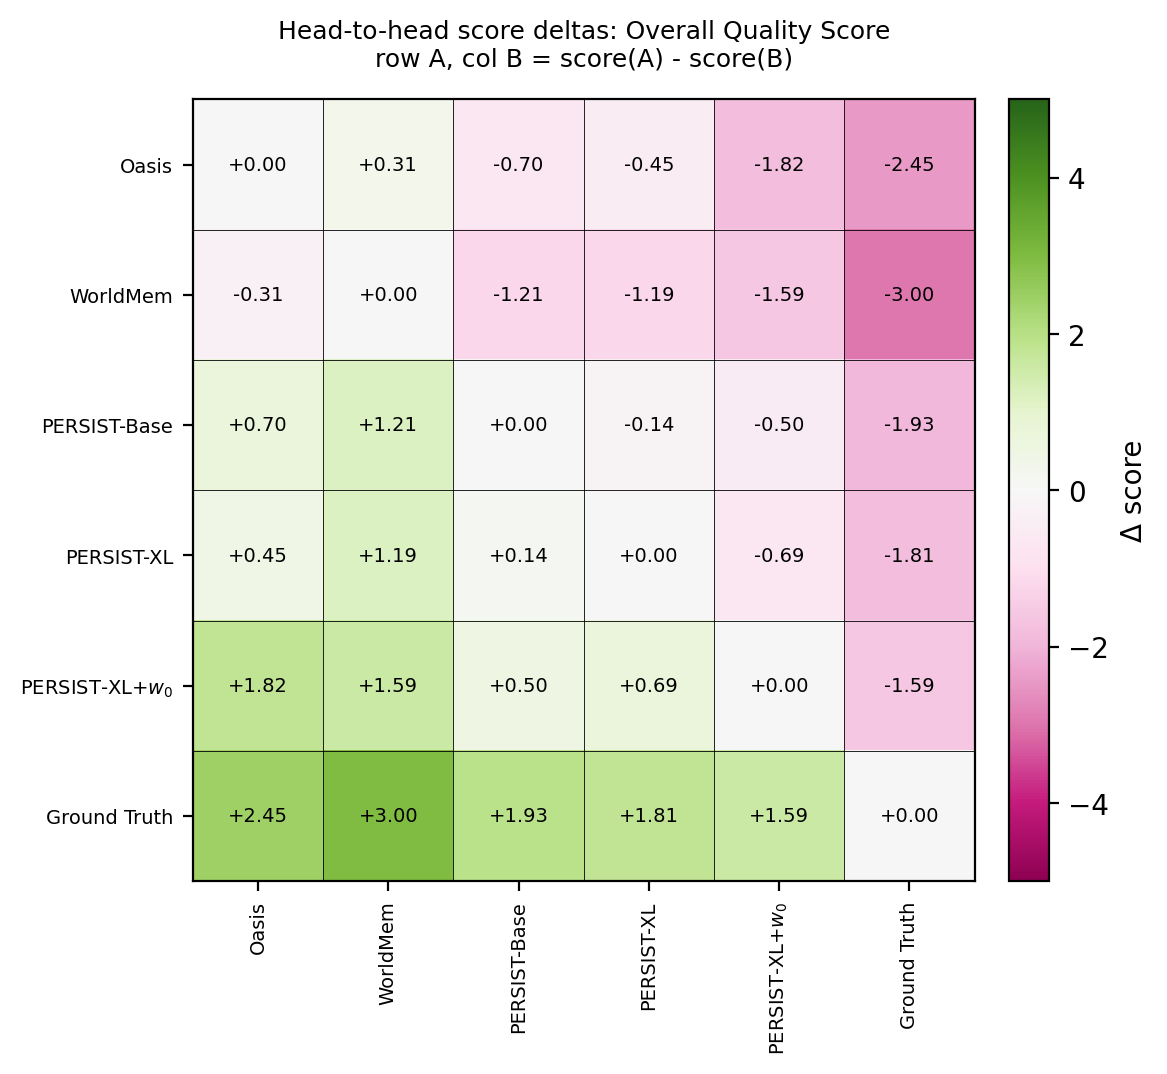
\includegraphics[width=\linewidth]{figs/h2h_png/h2h_metric_d.png}
        \caption{\textbf{Overall quality score}}
        \label{c4:fig:hth_d}
    \end{subfigure}

    \caption{Score differences during head-to-head comparisons across evaluation metrics.}
    \label{c4:fig:hth_all}
\end{figure}


\begin{algorithm}[htb!]
\centering
\caption{PERSIST inference logic.}\label{c4:alg:PERSIST}
\begin{algorithmic}[1]
\Input{Models $\gW_\theta$, $\gC_\theta$, $\gP_\theta$, 2D-VAE, 3D-VAE, \\ Model context window sizes $K_{\gW}$, $K_{\gC}$, $K_{\gP}$, \\ 
Renderer $\gR$, \\
Initial conditions $o_\text{init}$, $c_\text{init}$, \\
Episode Length $T$, \\
Agent.}
\State{$a_\text{init}\leftarrow \text{NO-OP}$} \Comment{Pipeline is always initialised using a NO-OP action.}
\State{$\bar{o}_0 \leftarrow \text{2D-VAE.encode}(o_\text{init})$}
\State{$\bar{w}_0 \leftarrow \gW_\theta (a_\text{init}, c_\text{init}, \bar{o}_0)$}
\State{$w_0 \leftarrow \text{3D-VAE.decode}(\bar{w}_0)$}
\State{$w_{{2D}_0} \leftarrow \gR(w_0,c_\text{init})$}
\State{$\bar{o}_0 \leftarrow \gP (w_{{2D}_0}, a_\text{init}$)} \Comment{Regenerating the starting observation from $w_0$ guarantees alignment between $w_0$ and $o_0$.}
\State{$o_0 \leftarrow \text{2D-VAE.decode}(\bar{o}_0)$}
\State{Initialise rollout buffers $\{A,C,O,\bar{O},W,\bar{W},W_{2D}\}$ with $a_\text{init},c_\text{init},o_0,\bar{o}_0,w_0,\bar{w}_0,w_{{2D}_0}$}
\For{$t$ in $1,\dots,T$}
\State{Append to $A$: $a_t \leftarrow \text{Agent}(o_{t-1})$}
\State{Append to $\bar{W}$: $\bar{w}_t \leftarrow \gW_\theta(\bar{W}^{t-1}_{t-K_\gW}, A^t_{t-K_\gW}, C^{t-1}_{t-K_\gW-1}, \bar{O}^{t-1}_{t-K_\gW-1})$}
\State{Append to $W$: $w_t \leftarrow \text{3D-VAE.decode}(\bar{w}_t)$}
\State{Append to $C$: $c_t \leftarrow \gC_\theta (C^{t-1}_{t-1-K_\gC}, W^t_{t-K_\gC}, A^t_{t-K_\gC})$}
\State{Append to $W_{2D}$: $w_{{2D}_t} \leftarrow \gR(w_t,c_t)$}
\State{Append to $\bar{O}$: $\bar{o}_t \leftarrow \gP_\theta ({W_{2D}}_{t-K_\gP}^{t}, A^t_{t-K_\gP}, \bar{O}^{t-1}_{t-K_\gP})$}
\State{Append to $O$: $o_t \leftarrow \text{2D-VAE.decode}(\bar{o}_t)$}
\EndFor
\end{algorithmic}
\end{algorithm}


\begin{algorithm}[htb!]
\centering
\caption{PERSIST$+w_0$ inference logic. \textcolor{blue}{Changes to \Cref{c4:alg:PERSIST} in blue.}}\label{c4:alg:PERSIST-w0}
\begin{algorithmic}[1]
\Input{Models $\gW_\theta$, $\gC_\theta$, $\gP_\theta$, 2D-VAE, 3D-VAE, \\ Model context window sizes $K_{\gW}$, $K_{\gC}$, $K_{\gP}$, \\ 
Renderer $\gR$, \\
Initial conditions $o_\text{init}$, $c_\text{init}$, \textcolor{blue}{$w_\text{init}$} \\
Episode Length $T$, \\
Agent.}
\State{$a_\text{init}\leftarrow \text{NO-OP}$} \Comment{Pipeline is always initialised using a NO-OP action.}
\State{$\bar{o}_0 \leftarrow \text{2D-VAE.encode}(o_\text{init})$}
\ColorState{blue}{$\bar{w}_0 \leftarrow \text{3D-VAE.encode}(w_\text{init})$}
\State{$w_{{2D}_0} \leftarrow \gR(\textcolor{blue}{w_\text{init}},c_\text{init})$}
\ColorState{blue}{$\bar{o}_0 \leftarrow \text{2D-VAE.encode}(o_\text{init})$}
\State{Initialise rollout buffers $\{A,C,O,\bar{O},W,\bar{W},W_{2D}\}$ with $a_\text{init},c_\text{init},\textcolor{blue}{o_\text{init}},\bar{o}_0,\textcolor{blue}{w_\text{init}},\bar{w}_0,w_{{2D}_0}$} \Comment{We can use $o_\text{init}$ directly as $o_\text{init}$ and $w_\text{init}$ are expected to be perfectly aligned.}
\For{$t$ in $1,\dots,T$}
\State{Append to $A$: $a_t \leftarrow \text{Agent}(o_{t-1})$}
\State{Append to $\bar{W}$: $\bar{w}_t \leftarrow \gW_\theta(\bar{W}^{t-1}_{t-K_\gW}, A^t_{t-K_\gW}, C^{t-1}_{t-K_\gW-1}, \bar{O}^{t-1}_{t-K_\gW-1})$}
\State{Append to $W$: $w_t \leftarrow \text{3D-VAE.decode}(\bar{w}_t)$}
\State{Append to $C$: $c_t \leftarrow \gC_\theta (C^{t-1}_{t-1-K_\gC}, W^t_{t-K_\gC}, A^t_{t-K_\gC})$}
\State{Append to $W_{2D}$: $w_{{2D}_t} \leftarrow \gR(w_t,c_t)$}
\State{Append to $\bar{O}$: $\bar{o}_t \leftarrow \gP_\theta ({W_{2D}}_{t-K_\gP}^{t}, A^t_{t-K_\gP}, \bar{O}^{t-1}_{t-K_\gP})$}
\State{Append to $O$: $o_t \leftarrow \text{2D-VAE.decode}(\bar{o}_t)$}
\EndFor
\end{algorithmic}
\end{algorithm}


\clearpage

\subsection{Scores for Each Evaluation Set}

\begin{table}[htb!]
\centering
\caption{Per set user study scores: \textbf{circle around}.}
\begin{adjustbox}{max width=\linewidth}
\begin{tabular}{lcccc}
\toprule
Method & Per Frame Visual Fidelity$\uparrow$ & 3D Consistency$\uparrow$ & Temporal Consistency$\uparrow$ & Overall Score$\uparrow$ \\
\midrule
Oasis & 2 $\pm$ 0.2 & 1.6 $\pm$ 0.2 & 1.5 $\pm$ 0.2 & 1.6 $\pm$ 0.2 \\
WorldMem & 1.7 $\pm$ 0.2 & 1.5 $\pm$ 0.1 & 1.3 $\pm$ 0.1 & 1.4 $\pm$ 0.1 \\
PERSIST-S & 2.8 $\pm$ 0.2 & 2.6 $\pm$ 0.2 & 2.3 $\pm$ 0.2 & 2.5 $\pm$ 0.2 \\
PERSIST & 3.0 $\pm$ 0.2 & 2.5 $\pm$ 0.1 & 2.2 $\pm$ 0.1 & 2.5 $\pm$ 0.1 \\
PERSIST$+w_0$ & \textbf{3.4 $\pm$ 0.2} & \textbf{3.0 $\pm$ 0.2} & \textbf{2.7 $\pm$ 0.3} & \textbf{3.1 $\pm$ 0.2} \\
\bottomrule
\end{tabular}
\end{adjustbox}
\label{c4:tab:user_study_scores_circle_around}
\end{table}

\begin{table}[htb!]
\centering
\caption{Per set user study scores: \textbf{free play}.}
\label{c4:tab:user_study_scores_free_play}
\begin{adjustbox}{max width=\linewidth}
\begin{tabular}{lcccc}
\toprule
Method & Per Frame Visual Fidelity$\uparrow$ & 3D Consistency$\uparrow$ & Temporal Consistency$\uparrow$ & Overall Score$\uparrow$ \\
\midrule
Oasis & 2.3 $\pm$ 0.2 & 2.2 $\pm$ 0.2 & 2.0 $\pm$ 0.2 & 2.0 $\pm$ 0.2 \\
WorldMem & 1.5 $\pm$ 0.2 & 1.5 $\pm$ 0.2 & 1.2 $\pm$ 0.1 & 1.3 $\pm$ 0.1 \\
PERSIST-S & 3.0 $\pm$ 0.2 & 2.9 $\pm$ 0.2 & 2.8 $\pm$ 0.2 & 3.0 $\pm$ 0.2 \\
PERSIST & 2.9 $\pm$ 0.2 & 2.8 $\pm$ 0.2 & 2.8 $\pm$ 0.2 & 2.8 $\pm$ 0.2 \\
PERSIST$+w_0$ & \textbf{3.6 $\pm$ 0.2} & \textbf{3.1 $\pm$ 0.2} & \textbf{3.3 $\pm$ 0.2} & \textbf{3.4 $\pm$ 0.2} \\
\bottomrule
\end{tabular}
\end{adjustbox}
\end{table}

\begin{table}[htb!]
\centering
\caption{Per set user study scores: \textbf{backwards and look around}.}\label{c4:tab:user_study_scores_backward_and_look_around}
\begin{adjustbox}{max width=\linewidth}
\begin{tabular}{lcccc}
\toprule
Method & Per Frame Visual Fidelity$\uparrow$ & 3D Consistency$\uparrow$ & Temporal Consistency$\uparrow$ & Overall Score$\uparrow$ \\
\midrule
Oasis & 1.9 $\pm$ 0.2 & 2.0 $\pm$ 0.2 & 2.0 $\pm$ 0.2 & 1.9 $\pm$ 0.2 \\
WorldMem & 1.7 $\pm$ 0.2 & 1.8 $\pm$ 0.2 & 1.6 $\pm$ 0.2 & 1.6 $\pm$ 0.1 \\
PERSIST-S & \textbf{3.0 $\pm$ 0.2} & \textbf{2.7 $\pm$ 0.2} & \textbf{2.7 $\pm$ 0.2} & 2.6 $\pm$ 0.2 \\
PERSIST & 2.7 $\pm$ 0.2 & 2.4 $\pm$ 0.2 & 2.4 $\pm$ 0.2 & 2.5 $\pm$ 0.1 \\
PERSIST$+w_0$ & \textbf{3.0 $\pm$ 0.2} & 2.6 $\pm$ 0.2 & 2.6 $\pm$ 0.2 & \textbf{2.8 $\pm$ 0.2} \\
\bottomrule
\end{tabular}
\end{adjustbox}
\end{table}

\begin{table}[htb!]
\caption{Per set user study scores: \textbf{forward and look around}.}
\label{c4:tab:user_study_scores_forward_and_look_around}
\centering
\begin{adjustbox}{max width=\linewidth}
\begin{tabular}{lcccc}
\toprule
Method & Per Frame Visual Fidelity$\uparrow$ & 3D Consistency$\uparrow$ & Temporal Consistency$\uparrow$ & Overall Score$\uparrow$ \\
\midrule
Oasis & 2.4 $\pm$ 0.2 & 2.0 $\pm$ 0.2 & 1.8 $\pm$ 0.2 & 1.9 $\pm$ 0.2 \\
WorldMem & 2.1 $\pm$ 0.2 & 2.2 $\pm$ 0.2 & 1.9 $\pm$ 0.2 & 1.9 $\pm$ 0.2 \\
PERSIST-S & 2.2 $\pm$ 0.2 & 2.3 $\pm$ 0.2 & 2.1 $\pm$ 0.2 & 2.3 $\pm$ 0.2 \\
PERSIST & 2.6 $\pm$ 0.2 & 2.3 $\pm$ 0.2 & \textbf{2.3 $\pm$ 0.2} & \textbf{2.4 $\pm$ 0.1} \\
PERSIST$+w_0$ & \textbf{2.7 $\pm$ 0.2} & \textbf{2.4 $\pm$ 0.2} & \textbf{2.3 $\pm$ 0.2} & \textbf{2.4 $\pm$ 0.2} \\\bottomrule
\end{tabular}
\end{adjustbox}
\end{table}


% \subsection{Cross domain evaluation}
% \todo[inline]{This should be linked to in main text. Here we would briefly motivate why we believe the cross domain analysis with Minedojo \& Craftium is valid. Acknowledge FVD is not great to compare across different domains. However show: 1) similar upper bound for FVD. 2) Show Users assign same scores to Minedojo / Craftium ground truth data.}

%\clearpage

\section{Inference Speed Evaluation}\label{c4:app:speed}

\begin{table}[h]
  \centering
  \caption{Inference speed comparison against baselines. All tests were conducted on a single A100 GPU with a batch size of 1 and 20 denoising steps.}
  \setlength{\tabcolsep}{4pt}
  \begin{tabular}{lc}
  \toprule
  Method & Time per frame (ms)$\downarrow$ \\
  \midrule
  PERSIST-S & \textbf{2672.4} \\
  Oasis & 3007.4 \\
  WorldMem & 6387.1 \\
  \bottomrule
  \end{tabular}
  \label{c4:tab:speed-baselines}
  \vspace{0.5cm}
\end{table}

We report inference speed comparisons of our PERSIST-S configuration against baselines in \Cref{c4:tab:speed-baselines}. Despite the additional overhead of tracking an explicit 3D state, PERSIST-S is faster because our implementation leverages key-value caching. We also provide a component-wise breakdown in \Cref{c4:tab:speed-components}. As expected, inference is dominated by the iterative denoising processes.

\begin{table}[h]
  \centering
  \caption{Component-wise breakdown of generation time per frame for PERSIST-S (20 denoising steps).}
  \setlength{\tabcolsep}{4pt}
  \begin{tabular}{lc}
  \toprule
  Component & Time per frame (ms) \\
  \midrule
  World frame & 1538.4 \\
  Pixel frame & 1111.0 \\
  Camera state & 21.9 \\
  Projection & 0.63 \\
  \bottomrule
  \end{tabular}
  \label{c4:tab:speed-components}
  \vspace{1cm}
\end{table}

Finally, we test an inference configuration of PERSIST-S employing 2 and 4 denoising steps for $\gW_\theta$ and $\gP_\theta$, respectively. This results in an inference speed of 886 ms (1.13 FPS), a $3\times$ improvement over employing 20 denoising steps. Interestingly, performance degradation is limited and generation remains stable without requiring any fine-tuning or timestep distillation; FVD increases from 159/170/179 to 207/230/244 at 200/400/600 frames.

While PERSIST does not yet run in real time, we are encouraged by the minimal performance degradation of PERSIST-S and its fast inference configuration compared to the base configuration. We expect that additional speedups achieved through increased spatial and temporal compression, smaller models, and more efficient implementations could enable PERSIST to achieve real-time interactivity. We leave this investigation to future work.

\section{Limitations and Future Work}\label{c4:app:limitations}

\textbf{Training without ground truth 3D supervision.} Our results underscore the critical role of explicit 3D representations in maintaining environmental coherence over long horizons. Currently, however, PERSIST acquires this representation via supervised training, restricting its applicability to simulators or datasets providing 3D annotations~\citep[e.g.][]{zhou2018stereo,Matterport3D,yeshwanth2023scannet++}. A key direction for future work is to relax this dependency by learning 3D representations directly from pixels, or by leveraging recent advances in 2D-to-3D foundation models~\citep{wang2025vggt,sam3dteam2025sam3d3dfyimages} to generate synthetic 3D annotations as a pre-processing step.

\textbf{Eliminating exposure bias.} While PERSIST yields substantial improvements in generation quality, temporal stability, and environmental coherence over baselines, human evaluators tend to prefer ground-truth videos in head-to-head comparisons, reporting a gradual degradation in visual quality and environment coherence over time. We attribute this degradation primarily to exposure bias: during training, individual pipeline components ($\gW_\theta$, $\gC_\theta$ and $\gP_\theta$) are trained using ground truth data; at inference, they condition on their own past predictions and on predictions from other components, causing a train-inference distribution mismatch that grows over time. We report examples of generation artifacts that occur over the course of a 2000-step episode in \Cref{c4:fig:limitations}. Leveraging PERSIST's fully differentiable pipeline, future work could explore incorporating an end-to-end post-training stage on generated rollouts, thereby aligning the training and inference distributions. As demonstrated in recent work~\citep{huang2025self}, this approach can be effective in making AR models robust to their own imperfect predictions.

\textbf{Unconstrained spatial memory.} PERSIST presently tracks a finite region of 3D space centred on the agent, causing information from distant locations to be discarded as the agent moves through the environment. To retain spatial information over arbitrarily large environments, future work could consider a conditioning strategy for $\gW_\theta$ based on loading spatial chunks from a 3D memory bank. Whereas pixel memory banks suffer from viewpoint redundancy, a 3D store is inherently deduplicated and spatially organized, offering unique advantages for efficient storage and retrieval of spatial information.

\begin{figure}
    \centering
    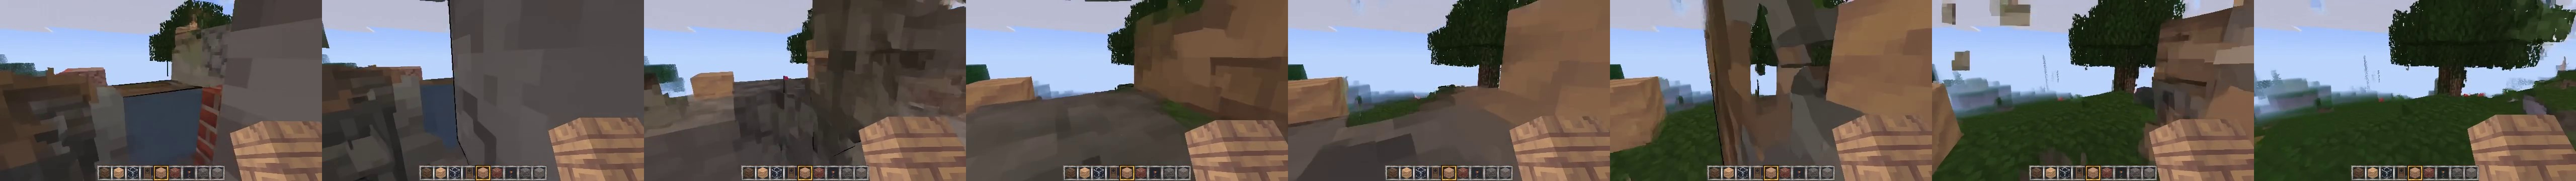
\includegraphics[width=1\linewidth]{figs/camera_clip.jpg}
    \caption{Conditioning on the
ground truth camera trajectory results in physical inconsistency with the world-frame, causing the agent to phase
through a wall.}
    \label{c4:fig:camera_clip}
\end{figure}


\begin{figure}[!htb]
  \begin{center}
    \centerline{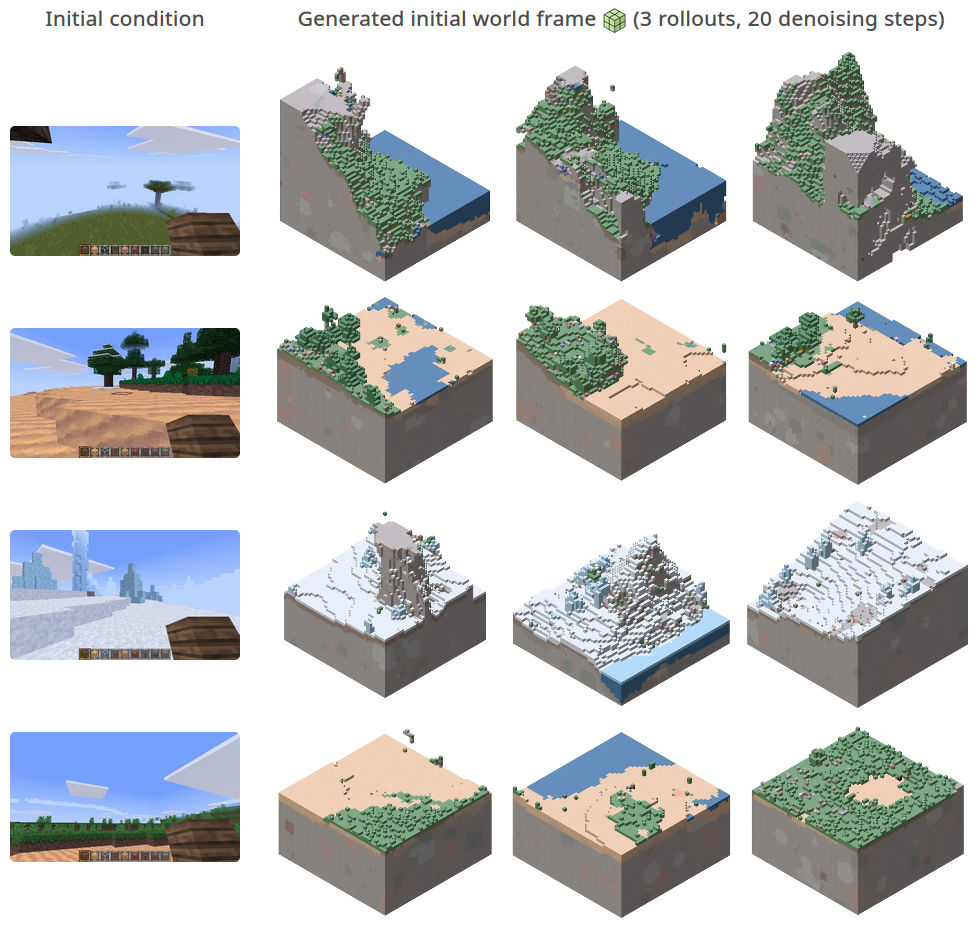
\includegraphics[width=0.75\linewidth]{figs/w0_generations.png}}
    \caption{PERSIST generates diverse but coherent initial world frames from a single RGB conditioning observation. Each row corresponds to a specific input RGB frame, while each column depicts the initial world frame sampled from $\gW_\theta$ during a specific generation episode.}
    \label{c4:fig:w0_gen}
  \end{center}
\end{figure}

\begin{figure}[!htb]
  \centering

  % helper length: (optional) tighten vertical spacing between rows
  \begin{minipage}{0.7\linewidth}
        \setlength{\tabcolsep}{0pt}

  % --- Row 1
  \noindent
  \begin{minipage}[c]{0.26\linewidth}
    \centering
    \begin{tcolorbox}[myimg,width=\linewidth]
    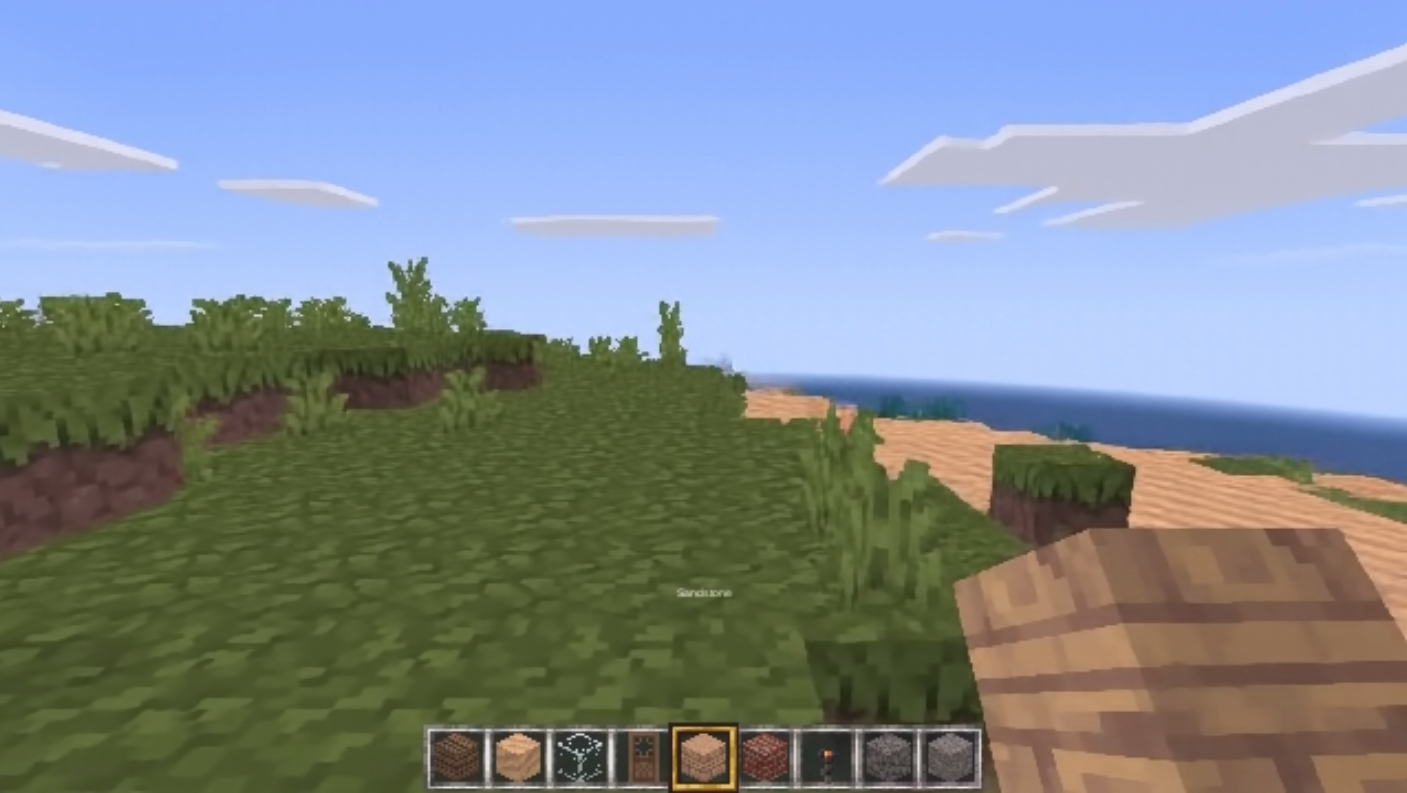
\includegraphics[width=\linewidth]{figs/limitations/s00.png}
    \end{tcolorbox}
  \end{minipage}\hfill
  \begin{minipage}[c]{0.55\linewidth}
    \textbf{Step 0 (0 seconds)}. Start of the episode. Generation is stable.
  \end{minipage}\par\vspace{0.1em}

  % --- Row 2
  \noindent
  \begin{minipage}[c]{0.26\linewidth}
    \centering
    \begin{tcolorbox}[myimg,width=\linewidth]
    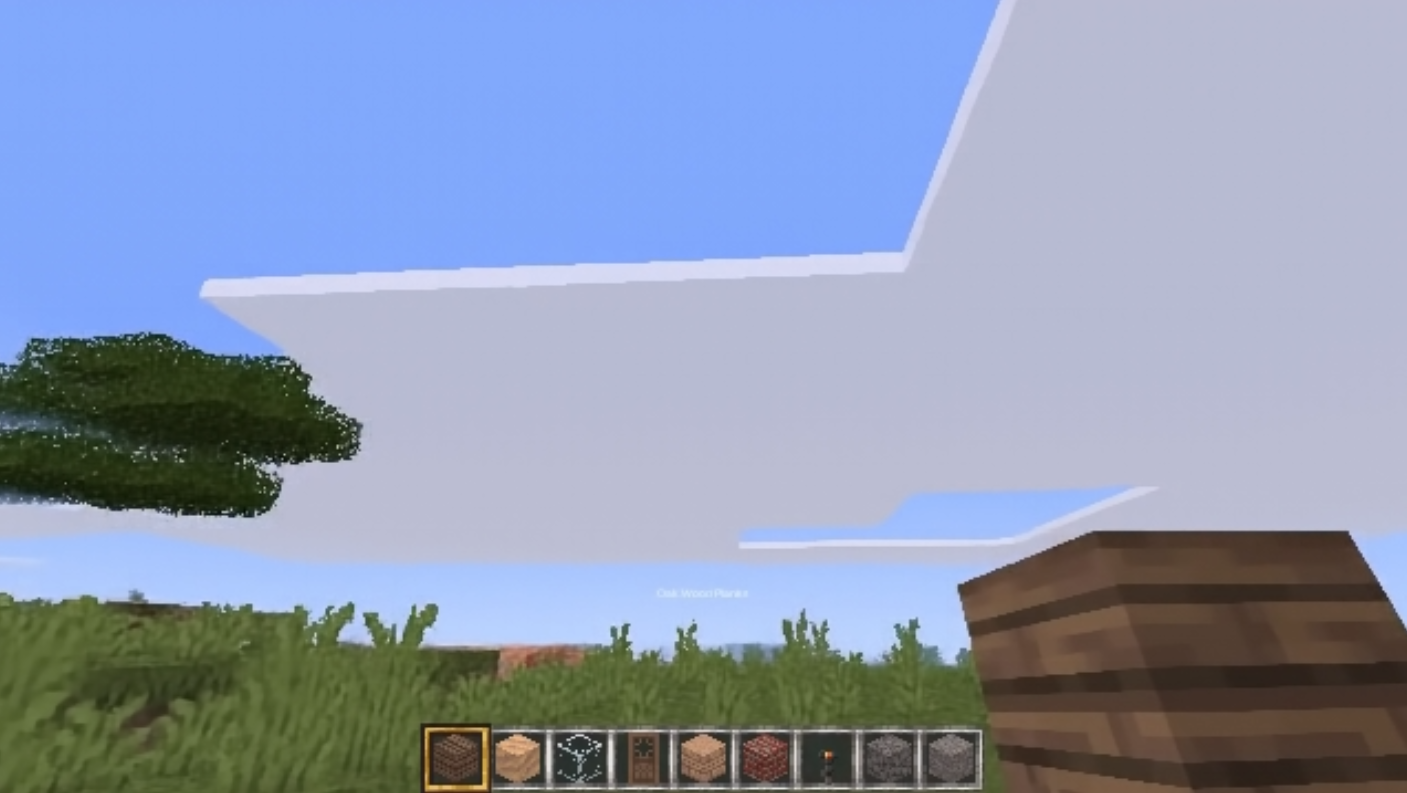
\includegraphics[width=\linewidth]{figs/limitations/s28.png}
    \end{tcolorbox}
  \end{minipage}\hfill
  \begin{minipage}[c]{0.55\linewidth}
    \textbf{Step 672 (28 seconds)}. A tree trunk disappears from the 3D representation. As a result only the tree foliage is rendered to the left of the agent.
  \end{minipage}\par\vspace{0.1em}

  % --- Row 3
  \noindent
  \begin{minipage}[c]{0.26\linewidth}
    \centering
    \begin{tcolorbox}[myimg,width=\linewidth]
    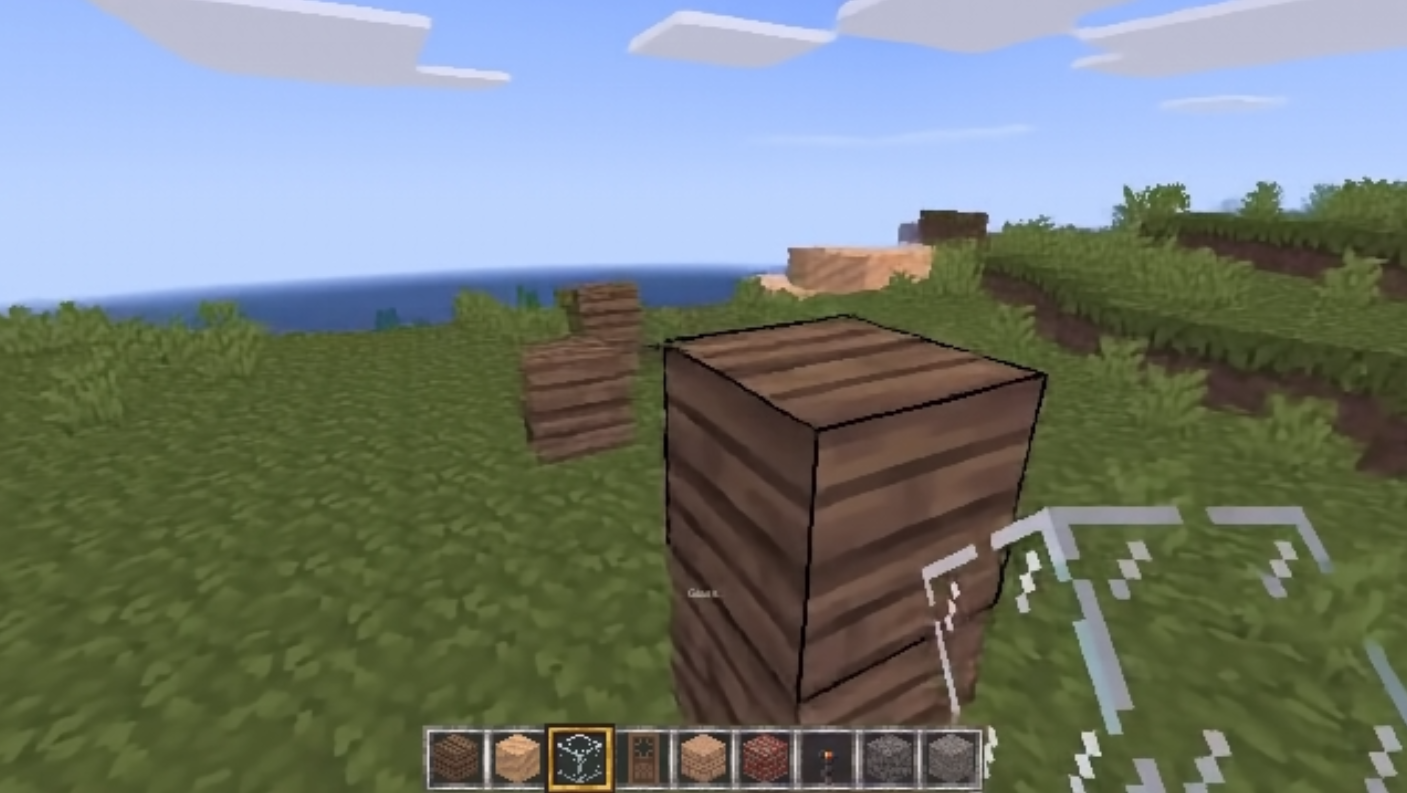
\includegraphics[width=\linewidth]{figs/limitations/s37.png}
    \end{tcolorbox}
  \end{minipage}\hfill
  \begin{minipage}[c]{0.55\linewidth}
    \textbf{Step 888 (37 seconds)}. Several wood blocks are wrongly predicted by $\gW_\vtheta$ and appear in the 3D representation. They get rendered in the agent's view.
  \end{minipage}\par\vspace{0.1em}

  % --- Row 4
  \noindent
  \begin{minipage}[c]{0.26\linewidth}
    \centering
    \begin{tcolorbox}[myimg,width=\linewidth]
    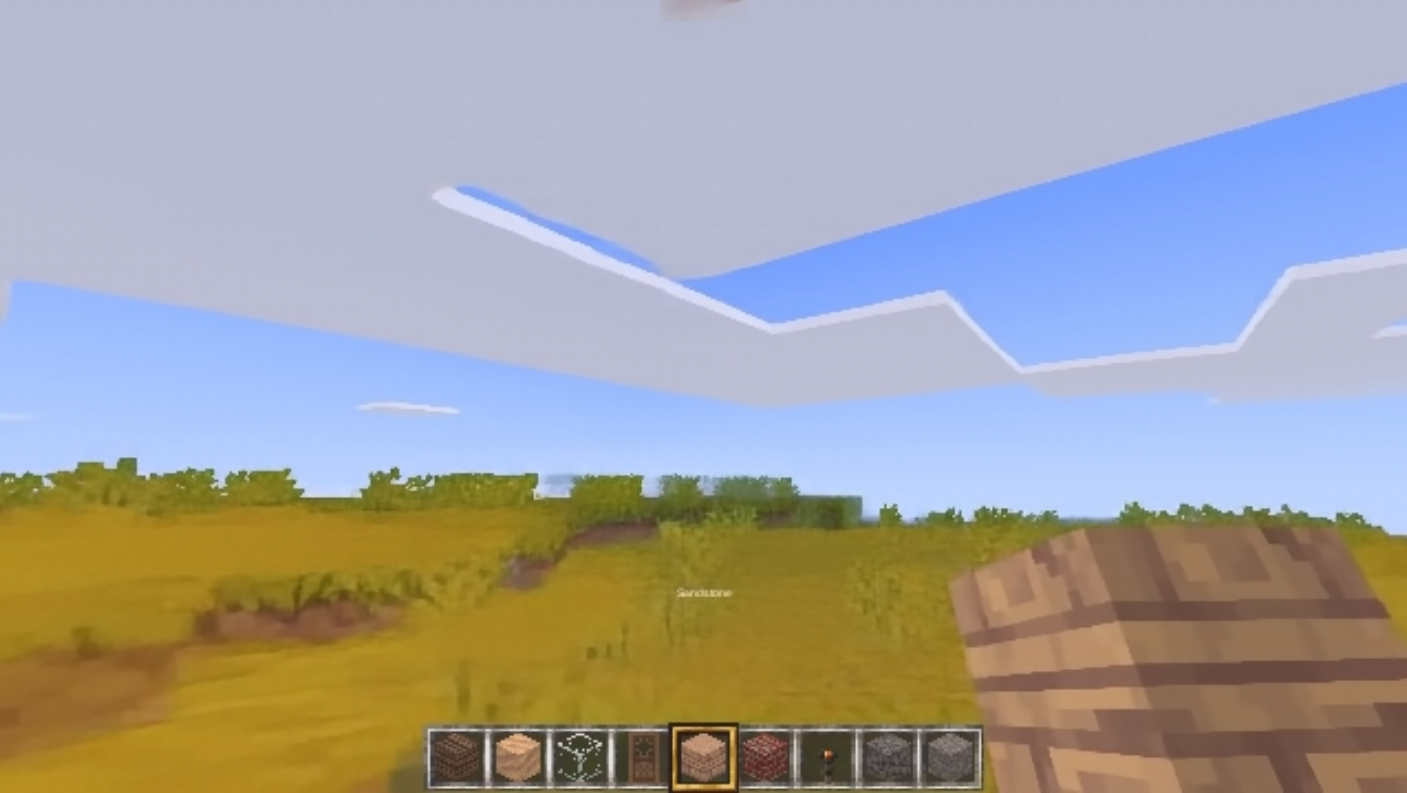
\includegraphics[width=\linewidth]{figs/limitations/s54.png}
    \end{tcolorbox}
  \end{minipage}\hfill
  \begin{minipage}[c]{0.55\linewidth}
    \textbf{Step 1296 (54 seconds)}. The texture of the ground is drifting to a yellowish colour. The 3D representation remains stable.
  \end{minipage}\par\vspace{0.1em}

  % --- Row 5
  \noindent
  \begin{minipage}[c]{0.26\linewidth}
    \centering
    \begin{tcolorbox}[myimg,width=\linewidth]
    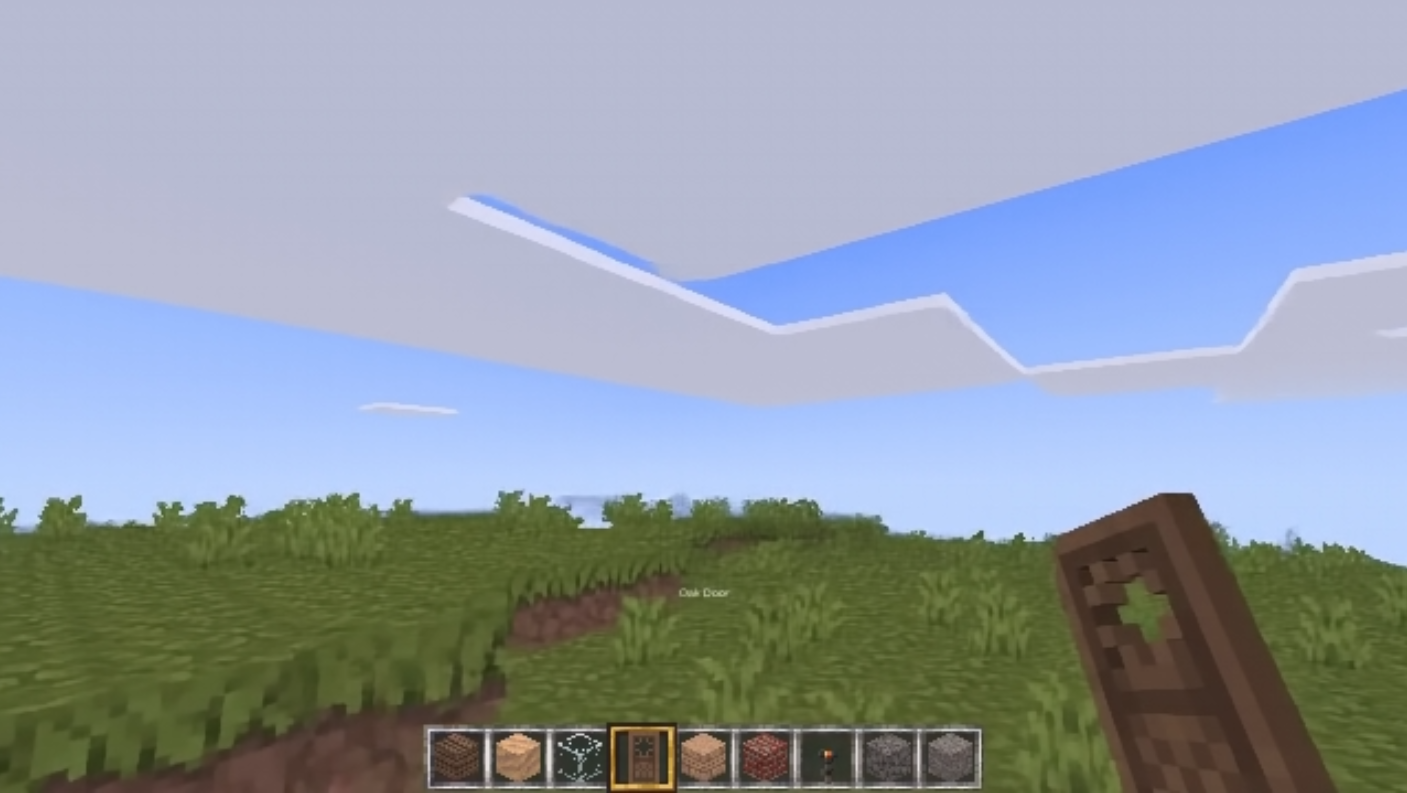
\includegraphics[width=\linewidth]{figs/limitations/s55.png}
    \end{tcolorbox}
  \end{minipage}\hfill
  \begin{minipage}[c]{0.55\linewidth}
    \textbf{Step 1320 (55 seconds)}. $\gP_\vtheta$ recovers the correct texture thanks to the grounding provided by $\vw_{2D}$.
  \end{minipage}\par\vspace{0.1em}

  % --- Row 6
  \noindent
  \begin{minipage}[c]{0.26\linewidth}
    \centering
    \begin{tcolorbox}[myimg,width=\linewidth]
    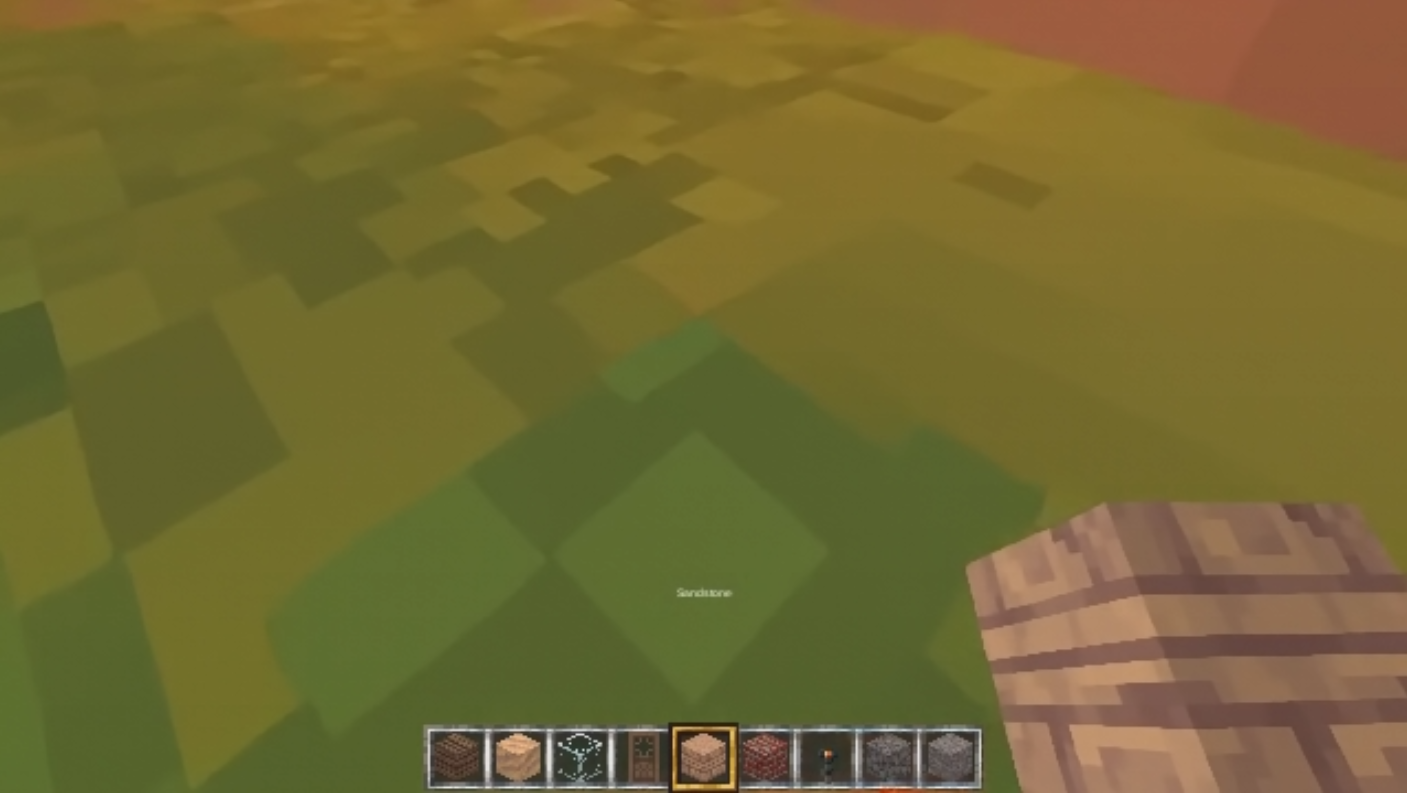
\includegraphics[width=\linewidth]{figs/limitations/s69.png}
    \end{tcolorbox}
  \end{minipage}\hfill
  \begin{minipage}[c]{0.55\linewidth}
    \textbf{Step 1656 (69 seconds)}. A collision gets mispredicted and the agent clips through a block. The ground texture begins to drift.
  \end{minipage}\par\vspace{0.1em}

  % --- Row 7
  \noindent
  \begin{minipage}[c]{0.26\linewidth}
    \centering
    \begin{tcolorbox}[myimg,width=\linewidth]
    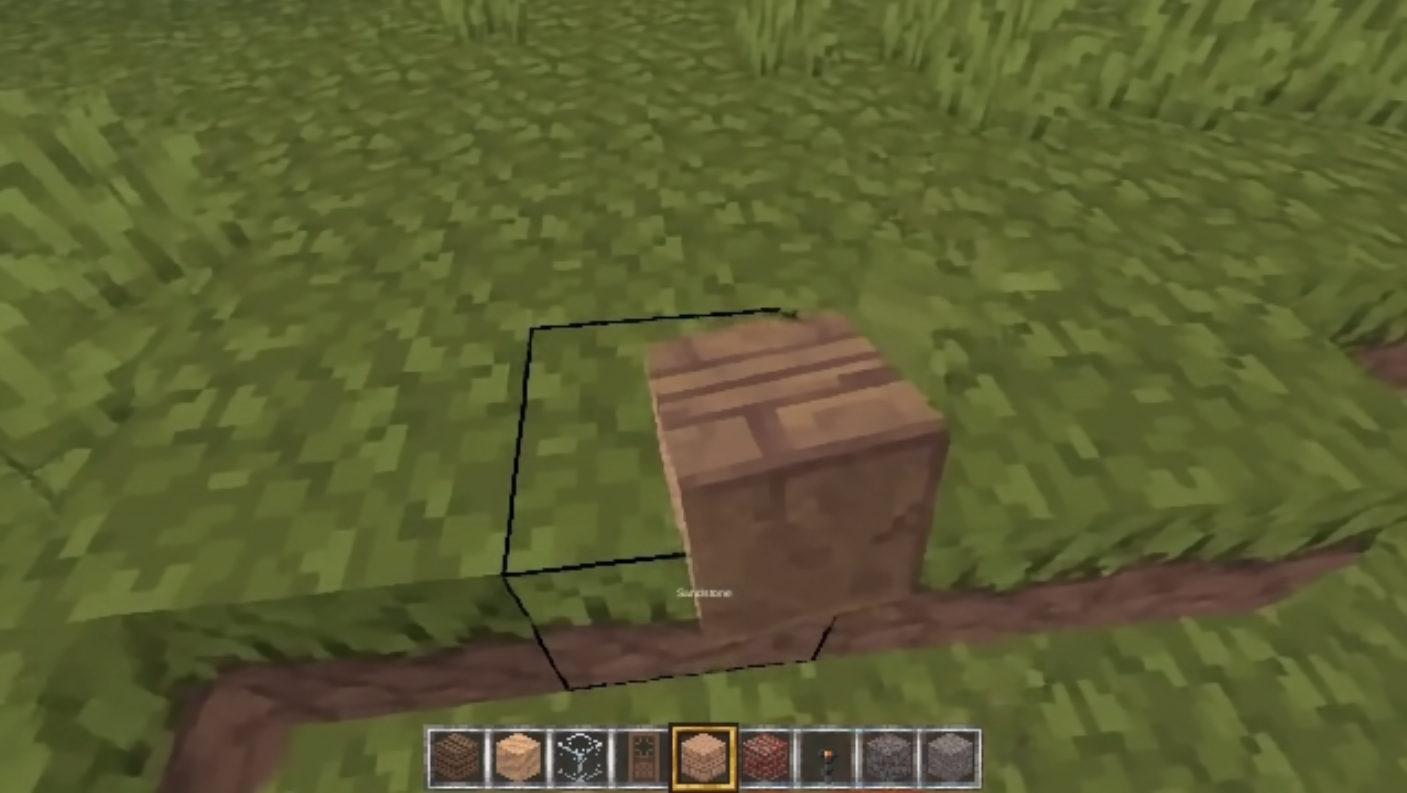
\includegraphics[width=\linewidth]{figs/limitations/s70.png}
    \end{tcolorbox}
  \end{minipage}\hfill
  \begin{minipage}[c]{0.55\linewidth}
    \textbf{Step 1680 (70 seconds)}. The model recovers from terrain clipping and texture drift after the agent executes a jump action.
  \end{minipage}\par\vspace{0.1em}

  % --- Row 8
  \noindent
  \begin{minipage}[c]{0.26\linewidth}
    \centering
    \begin{tcolorbox}[myimg,width=\linewidth]
    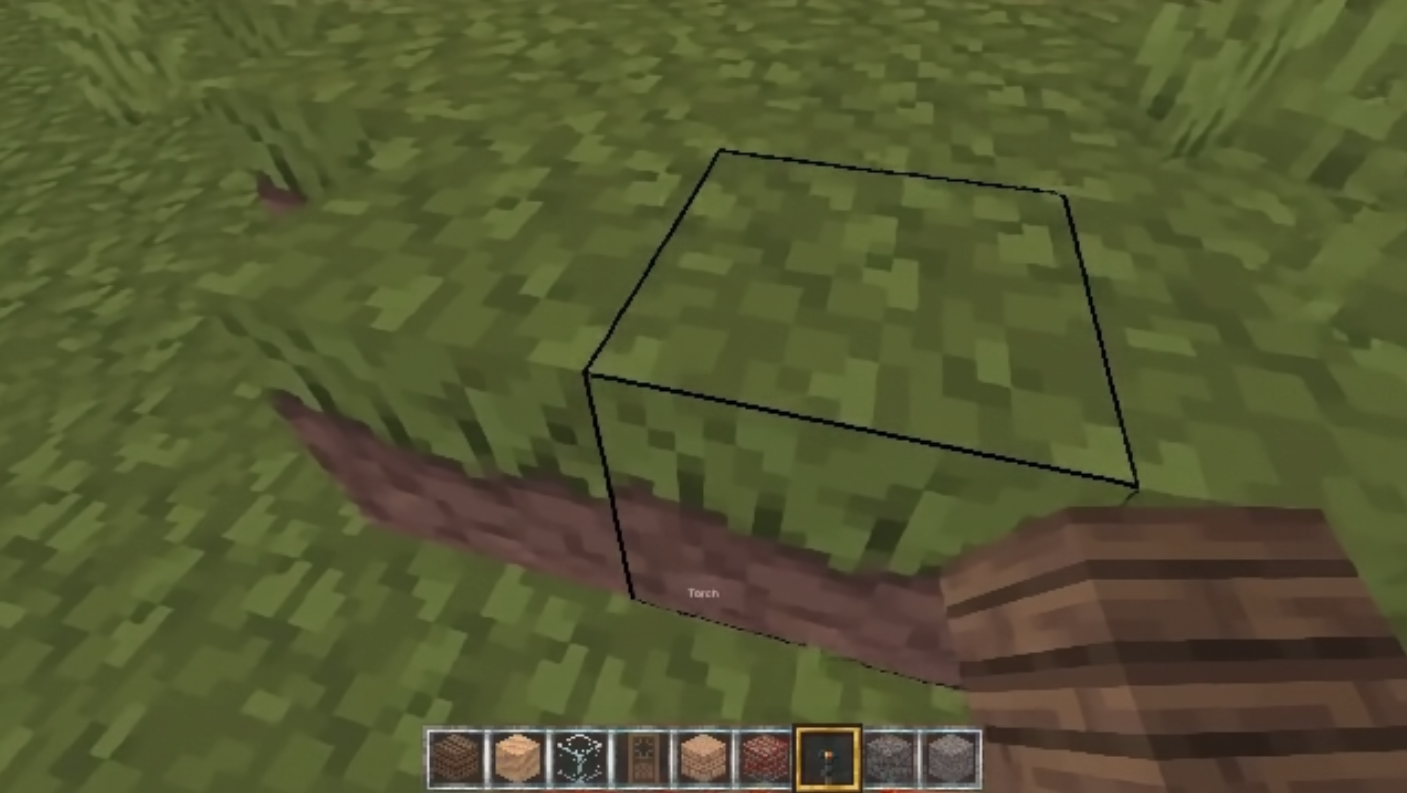
\includegraphics[width=\linewidth]{figs/limitations/s83.png}
    \end{tcolorbox}
  \end{minipage}\hfill
  \begin{minipage}[c]{0.55\linewidth}
    \textbf{Step 2000 (83 seconds)}. The episode concludes on a stable frame. The environment remains globally coherent after 2000 steps, but artifacts occur more frequently due to exposure bias.
  \end{minipage}
  \end{minipage}

\vspace{0.05cm}
  \caption{Generation artifacts and subsequent recoveries over a 2000-step (83 seconds) episode generated with PERSIST. The 3D representation drifts locally, causing individual blocks to appear and disappear from the agent's view. However we find that the 3D representation remains globally coherent and has a net stabilising effect on generation, allowing $\gP_\theta$ to recover from visual artifacts. This lets PERSIST generate rollouts lasting thousands of steps, even if glitches become more frequent over time due to autoregressive drift.}
  \label{c4:fig:limitations}
\end{figure}


%%%%%%%%%%%%%%%%%%%%%%%%%%%%%%%%%%%%%%%%%%%%%%%%%%%%%%%%%%%%%%%%%%%%%%%%%%%%%%%
%%%%%%%%%%%%%%%%%%%%%%%%%%%%%%%%%%%%%%%%%%%%%%%%%%%%%%%%%%%%%%%%%%%%%%%%%%%%%%%

\end{subappendices}

% This document was modified from the file originally made available by
% Pat Langley and Andrea Danyluk for ICML-2K. This version was created
% by Iain Murray in 2018, and modified by Alexandre Bouchard in
% 2019 and 2021 and by Csaba Szepesvari, Gang Niu and Sivan Sabato in 2022.
% Modified again in 2023 and 2024 by Sivan Sabato and Jonathan Scarlett.
% Previous contributors include Dan Roy, Lise Getoor and Tobias
% Scheffer, which was slightly modified from the 2010 version by
% Thorsten Joachims & Johannes Fuernkranz, slightly modified from the
% 2009 version by Kiri Wagstaff and Sam Roweis's 2008 version, which is
% slightly modified from Prasad Tadepalli's 2007 version which is a
% lightly changed version of the previous year's version by Andrew
% Moore, which was in turn edited from those of Kristian Kersting and
% Codrina Lauth. Alex Smola contributed to the algorithmic style files.
